\documentclass[11pt]{article}

% --- Encoding & fonts ---
\usepackage[utf8]{inputenc}
\usepackage[T1]{fontenc}
\usepackage{microtype}

% --- Math ---
\usepackage{amsmath,amssymb,amsfonts,amsthm}
\newtheorem{theorem}{Theorem}
\newtheorem{proposition}{Proposition}
\newtheorem{corollary}{Corollary}
\newtheorem{remark}{Remark}
\newtheorem{assumption}{Assumption}

% --- Layout ---
\usepackage[margin=1in]{geometry}
\usepackage[section]{placeins}
\setlength{\emergencystretch}{5em}

% Force \FloatBarrier before every \subsection and \subsubsection so floats
% cannot cross into the next (sub)subsection, eliminating orphan headings
% followed by tall whitespace (the \texttt{[section]} option of
% \texttt{placeins} only barriers at \section).
\let\origsubsection\subsection
\renewcommand{\subsection}{\FloatBarrier\origsubsection}
\let\origsubsubsection\subsubsection
\renewcommand{\subsubsection}{\FloatBarrier\origsubsubsection}

% --- Floats, tables, figures ---
\usepackage{graphicx}
\usepackage{float}
\usepackage{booktabs}
\usepackage{multirow}
\usepackage{caption}
\usepackage{subcaption}

% --- Aggressive float packing (relaxed defaults to avoid sparse pages) ---
\renewcommand{\topfraction}{0.95}
\renewcommand{\bottomfraction}{0.85}
\renewcommand{\textfraction}{0.05}
\renewcommand{\floatpagefraction}{0.75}
\renewcommand{\dbltopfraction}{0.95}
\renewcommand{\dblfloatpagefraction}{0.75}
\setcounter{topnumber}{3}
\setcounter{bottomnumber}{2}
\setcounter{totalnumber}{5}

% --- Algorithms, lists, color ---
\usepackage{algorithm}
\usepackage{algorithmic}
\usepackage{enumitem}
\usepackage{xcolor}

% breakablealgorithm: a non-floating algorithm environment that can split
% across pages. Use in place of \begin{algorithm} for any algorithm body
% taller than a single page; \caption / \label / counter increments still
% work as in the floating version.
\makeatletter
\newenvironment{breakablealgorithm}
  {\begin{center}
    \refstepcounter{algorithm}%
    \hrule height.8pt depth0pt \kern2pt%
    \renewcommand{\caption}[2][\relax]{%
      {\raggedright\textbf{\ALG@name~\thealgorithm} ##2\par}%
      \ifx\relax##1\relax%
        \addcontentsline{loa}{algorithm}{\protect\numberline{\thealgorithm}##2}%
      \else%
        \addcontentsline{loa}{algorithm}{\protect\numberline{\thealgorithm}##1}%
      \fi%
      \kern2pt\hrule\kern2pt%
    }%
  }{\kern2pt\hrule\relax%
   \end{center}%
  }
\makeatother

% --- TikZ ---
\usepackage{tikz}
\usetikzlibrary{shapes.geometric,arrows.meta,positioning,fit,calc,decorations.pathreplacing}

% --- Bibliography ---
\usepackage[numbers,sort&compress]{natbib}

% --- Links (load last) ---
\usepackage{hyperref}
\hypersetup{
    colorlinks=true,
    linkcolor=blue,
    citecolor=blue,
    urlcolor=blue,
    pdftitle={Continuous Hidden Markov Models for Equity Returns: Heavy-Tail Emission Families and Regime-Conditional Value-at-Risk},
    pdfauthor={Abdulrahman Alswaidan, Cade Jin, Jeffrey D. Varner},
    pdfsubject={CHMM synthetic-data generator for daily US-equity returns},
    pdfkeywords={CHMM, Baum-Welch, Student-t emissions, semi-Markov, stylized facts, copula, Value-at-Risk, Kupiec, synthetic data}
}
\makeatletter
\g@addto@macro\UrlBreaks{\do\-\do\_}
\makeatother

% --- Caption style (V10/V11, 2026-04-22) ---
% Top-of-table labels, bold table/figure tags, small font for captions and subcaptions.
\captionsetup{labelfont=bf, labelsep=period, font=small, justification=justified}
\captionsetup[sub]{labelfont=bf, font=small, labelformat=parens, labelsep=space}

% --- Custom commands ---
\newcommand{\R}{\mathbb{R}}
\newcommand{\E}{\mathbb{E}}
\newcommand{\Prob}{\mathbb{P}}

% --- Project-level numeric macros (V10/V11 bundle, 2026-04-22) ---
% Consistent formatting for recurring numeric constructs.
% Use in new prose and tables; legacy cells may be migrated gradually (see V16
% siunitx migration in plan-equity-paper.md for the bulk pass).
\newcommand{\pct}[1]{\ensuremath{#1\%}}
\newcommand{\Kdisc}[1]{\ensuremath{K_{\text{disc}} = #1}}
\newcommand{\LRuc}[1]{\ensuremath{\text{LR}_{\text{uc}} = #1}}
\newcommand{\NPaths}[1]{\ensuremath{N_{\text{paths}} = #1}}
\newcommand{\TIS}[1]{\ensuremath{T_{\text{IS}} = #1}}
\newcommand{\TOoS}[1]{\ensuremath{T_{\text{OoS}} = #1}}

\title{Continuous Hidden Markov Models for Equity Returns:\\ Heavy-Tail Emission Families\\ and Regime-Conditional Value-at-Risk}

\author{
    Abdulrahman Alswaidan\thanks{Cornell University, Robert Frederick Smith School of Chemical and Biomolecular Engineering, Ithaca, NY, USA. Email: \texttt{aa2725@cornell.edu}.}
    \and
    Cade Jin\thanks{Cornell Ann S.\ Bowers College of Computing and Information Science, Cornell University, Ithaca, NY, USA. Email: \texttt{cj383@cornell.edu}.}
    \and
    Jeffrey D.\ Varner\thanks{Cornell University, Robert Frederick Smith School of Chemical and Biomolecular Engineering, Ithaca, NY, USA. Email: \texttt{jdv27@cornell.edu}.}
}

\date{\today}

\begin{document}

\maketitle

% ========================================================================================= %
\begin{abstract}
We present a continuous hidden Markov model (CHMM) framework for daily US-equity returns. The textbook bilinear identity for the absolute-return autocorrelation function recasts the empirical Ryd\'{e}n et al.\ low-$K$ failure as an effective-rank statement on the centred transition matrix $\mathbf T - \mathbf 1\bar{\boldsymbol\pi}^\top$. An empirical diagnostic on the fitted estimator $\hat{\mathbf T}$ shows the implied $K - 1$ rank bound is non-binding at the cross-ticker median for $K \ge 3$, with the bound still doing visible work on the left tail of the distribution (minimum dominant-mode share $32.6\%$ on NEM).

A unified ECM scaffold supports four emission families (Gaussian, Student-$t$, Laplace, Generalised Error Distribution) with shared forward-backward recursions and quantile-based initialisation; the M-step is the only architectural difference. The empirical study covers SPY 2014 to 2026, a sector-balanced 30-ticker panel, a CRSP cross-decade transfer (1994 to 2004 in-sample, 2004 to 2006 out-of-sample), and a six-asset US-equity copula extension.

Headline operating result: a regime-conditional Value-at-Risk that propagates the one-step-ahead state forecast through the predictive mixture passes the Christoffersen joint conditional-coverage test cleanly at $\alpha = 0.05$ across emission families on the headline out-of-sample window and on $19/24$ rows of a six-fold rolling-origin walk-forward; rejections concentrate on out-of-distribution stress folds. At $\alpha = 0.01$ the Engle-Manganelli dynamic-quantile backstop rejects $K = 18$ on the headline window, so the strict-tail Christoffersen pass is power-driven.

Positioning is honest. The i.i.d.\ bootstrap and a maximum-likelihood hidden semi-Markov model both exceed the CHMM on raw single-window out-of-sample Kolmogorov-Smirnov. The CHMM value-add is the structural use cases that those alternatives cannot serve (regime-conditional VaR, multi-asset copula composition, parametric synthetic-data privacy), together with a unified emission-family ablation. The single-window OoS sits at the upper tail of a six-fold rolling-origin walk-forward whose median CHMM-N OoS KS is $62.1\%$ at $K^\star = 3$, the operationally informative summary. Scope is daily US equities under stationary OoS; a non-equity stress test on GLD collapses under static fitting, and periodic refit is the deployment recipe.
\end{abstract}

\noindent\textbf{Keywords:} Continuous Hidden Markov Model, Baum-Welch, Student-$t$ Emissions, Stylized Facts, Volatility Clustering, Value-at-Risk, Synthetic-Data Generator.

% ========================================================================================= %
\section{Introduction}
\label{sec:introduction}
Synthetic generators of equity-return time series support stress testing, regulatory backtesting, scenario design, and the training of machine-learning models on data that cannot be released for privacy or licensing reasons~\cite{jordon2022synthetic, assefa2020generating, alswaidan2026hybrid}. A useful generator has to reproduce, at the same time, the standard stylized facts of daily returns: heavy-tailed marginals, negligible linear autocorrelation, and slow decay of the autocorrelation function (ACF) of absolute returns~\cite{mandelbrot1963variation, cont2001empirical}. Generalised autoregressive conditional heteroskedasticity (GARCH) models~\cite{engle1982autoregressive, bollerslev1986generalized} capture volatility clustering but not the multi-regime structure of the marginal; i.i.d.\ generators match the marginal but lose temporal persistence; deep generators~\cite{yoon2019timegan, wiese2020quantgan, rasul2021autoregressive} reproduce some stylized facts at the cost of interpretability and reproducibility. One negative result has shaped two decades of work on regime-switching models. \citet{ryden1998stylized} fitted Gaussian-emission hidden Markov models (HMMs) at low state counts and concluded that the geometric sojourn-time distribution of a standard Markov chain makes the ACF decay too fast to match the observed slow decay; \citet{bulla2006stylized} recovered the ACF fit by replacing the Markov chain with a hidden semi-Markov chain, at the cost of much greater complexity. The Ryd\'{e}n et al.\ failure combines two constraints: a temporal one (the absolute-return ACF must allow slow-decay modes) and a distributional one (the marginal mixture must carry enough components to match observed kurtosis). A standard closed-form identity for the absolute-return ACF, written as a sum over the non-unit eigenvalues of the transition matrix~\cite{hamilton1994time, krolzig1997markov, timmermann2000moments}, bounds the number of decay modes by the rank of the centred transition matrix. We ask whether that bound actually matters on equity-return data once enough latent states are allowed.

In this study, we built three things on top of the continuous HMM (CHMM): a unified expectation-conditional-maximisation (ECM) framework for the four emission families, in which only the M-step changes between variants; a regime-conditional Value-at-Risk (VaR) that averages the predictive density over the one-step-ahead state forecast; and a Student-$t$ copula that ties the per-asset CHMM marginals into a joint generator through Sklar's theorem. We tested the model four ways: a six-fold rolling-origin walk-forward on the SPY decade, a sector-balanced 30-ticker panel across ten Global Industry Classification Standard (GICS) sectors, a Center for Research in Security Prices (CRSP) cross-decade transfer, and a six-asset US-equity basket, which together guard against single-window over-fitting. The four-family panel reproduced all three symmetric Cont stylized facts at the chosen $K^\star$, and heavy-tailed emissions narrowed the kurtosis gap relative to the Gaussian baseline. The rank bound from the bilinear ACF identity did not bind at the cross-ticker median, though it still mattered for a few tickers that introduced new regimes. The regime-conditional VaR passed the Christoffersen joint conditional-coverage test cleanly on the main window and on most walk-forward folds, and the Student-$t$ copula matched off-diagonal correlations far better than the single-index alternative. We read this to mean that the Ryd\'{e}n low-$K$ failure is a limit on the marginal mixture, not on the chain's temporal structure, once initialisation is fixed and the emissions can carry heavy tails. The i.i.d.\ bootstrap and a maximum-likelihood hidden semi-Markov model (HSMM) beat the CHMM on raw single-window distributional fit, but neither supports the regime-conditional risk forecasting, multi-asset copula composition, or parametric synthetic-data privacy the CHMM is built for. The scope is daily US equities: a non-equity stress test on the GLD exchange-traded fund (ETF) breaks down under static fitting, and we recommend periodic refit within that scope.


\section{Related Work}
\label{sec:related}
\paragraph{Stylized facts and parametric volatility.}
The canonical set of stylized facts \cite{cont2001empirical}, namely heavy tails \cite{mandelbrot1963variation}, absence of linear autocorrelation \cite{fama1970efficient}, and slow decay of the absolute-return ACF \cite{schwert1989does, ding1993long, andersen1997heterogeneous}, must be reproduced jointly for a generator to be useful downstream.
Autoregressive conditional heteroscedasticity (ARCH) and its generalised variant (GARCH) \cite{engle1982autoregressive, bollerslev1986generalized} encode volatility persistence through a single decay parameter but impose a unimodal innovation distribution and, as we confirm, fail distributional tests on equity returns.
Jump-diffusion models \cite{merton1976option, kou2002jump} generate heavy tails but lack a clustering mechanism: after a jump the conditional variance returns immediately to baseline; \citet{maheu2004news} couple jumps with a regime-switching volatility component to address this, an alternative route to regime-dependent tails that our CHMM-t scaffold addresses through heavy-tailed emissions rather than an explicit jump process.
Maximum-likelihood fitting of heavy-tailed innovations in a latent-volatility framework has been studied for stochastic-volatility-in-mean models by \citet{abantovalle2017svm}, who compare Normal, Student-t, generalized error distribution (GED), and Slash errors; our CHMM-t and CHMM-L are the HMM analog of that emission-family choice.

\paragraph{Regime-switching and the Ryd\'{e}n et al.\ limitation.}
\citet{hamilton1989new} introduced Markov-switching models to economics, and \citet{schaller1997regime} provided an early demonstration that monthly equity returns from the Center for Research in Security Prices (CRSP) are well-described by a two-state Markov-switching specification with strongly different mean and variance between regimes; \citet{angbekaert2002regime} subsequently showed that short-rate dynamics in several developed markets also admit a regime-switching representation, establishing regime-switching as a cross-asset-class phenomenon rather than one confined to macro series or equities.
The seminal evaluation of HMMs against the Cont stylized facts is due to \citet{ryden1998stylized}, who fitted Gaussian-emission HMMs with $K = 2$--$3$ states to daily equity-index return series and showed that the geometric sojourn-time distribution of a standard Markov chain produces exponential ACF decay too fast to match the observed slow decay.
\citet{bulla2006stylized} restored fidelity with hidden semi-Markov models (HSMMs) that replace the geometric sojourn distribution with flexible alternatives.
\citet{alswaidan2026hybrid} instead kept the discrete HMM framework and introduced a Poisson jump-duration process to force dwell time in tail states.

Within the same family, \citet{nguyen2018hidden} applies a four-state continuous HMM to monthly S\&P~500 prices for OoS trading signal generation, selecting the state count through the AIC, BIC, HQC, and CAIC information criteria.
We adopt the same four-criterion selection (Section~\ref{sec:model_selection}), in addition to our multi-metric distributional score, to place the $K$-sweep recommendation on standard statistical footing.

Consistent with this broader regime-switching literature, we find that at $K \geq 3$ with quantile-based initialization the Baum-Welch algorithm learns heterogeneous self-transition probabilities across regimes, and the resulting mixture of $K$ geometric sojourn-time distributions approximates slow ACF decay.
This moderate-$K$ route complements the HSMM \citep{bulla2006stylized} and jump-augmented \citep{alswaidan2026hybrid} corrections to the Ryd\'{e}n et al.\ result rather than superseding them; the integrative contribution of this paper is the unified log-space EM scaffold shared by the three emission variants, the twelve-generator evaluation panel, and the regime-conditional VaR test (Section~\ref{sec:var_backtest}), not a single-route resolution of the Ryd\'{e}n limitation.

\paragraph{Discrete HMM with jumps.}
The immediate predecessor of this paper, \citet{alswaidan2026hybrid}, discretizes returns into Laplace quantile bins, estimates $\mathbf{T}$ by frequency counting, fits bin-conditional Student-t emissions, and adds a Poisson jump-duration process with two grid-calibrated hyperparameters ($\epsilon, \lambda$).
The continuous model presented here offers a simpler alternative on each of three axes: no binning, a single EM step in which Baum-Welch jointly learns transitions and emissions (instead of a separate frequency-counted $\mathbf{T}$ plus within-bin emission fit), and no jump mechanism at moderate $K$; this is a modelling-cost comparison rather than a claim that the discrete-plus-jumps route is inferior for the tasks it was designed for.

\paragraph{Cross-asset dependence.}
For multi-asset synthesis, the Single Index Model \cite{sharpe1963simplified} propagates a market factor through a rank-one linear decomposition but distorts each non-market marginal; Sklar's theorem \cite{sklar1959fonctions, nelsen2006introduction} supports a cleaner decomposition in which each asset's fitted marginal is kept and only the copula is estimated.
Gaussian and Student-t copulas \cite{demarta2005tcopula, mcneil2015quantitative} are the standard choices, and rank-reordering simulation \cite{iman1982distribution} injects the copula dependence onto pre-simulated marginal paths without distorting any marginal.
We confirm, on continuous CHMM marginals, the copula-ahead-of-SIM ordering reported by \citet{alswaidan2026hybrid} for discrete HMM marginals, which suggests that the ordering is intrinsic to the rank-reordering construction rather than specific to the marginal model.

\paragraph{Deep generative models and quality assessment.}
Generative adversarial network (GAN) based generators reproduce the visual appearance of return series but typically fail the clustering test unless architectures encode temporal dependence explicitly \cite{takahashi2019modeling, kwon2024can}, the TimeGAN family of \citet{yoon2019timegan} being the standard reference in this direction; neural baselines in \citet{alswaidan2026hybrid} close most of the ACF gap but suffer variance collapse, indicating that the distribution--clustering tension remains in tension for neural approaches.
Following the GRU baseline used in \citet{alswaidan2026hybrid}, we add a single-layer GRU + Gaussian-head auto-regressive recurrent generator (Section~\ref{sec:benchmarks}) to Table~\ref{tab:model_comparison} as a deep-generative head-to-head row, trained by negative log-likelihood on the IS series and rolled forward by sampling from the predicted Gaussian and feeding the sample back into the recurrence.
For evaluation, we adopt the category framework of \citet{stenger2024thinking} and the financial-synthesis emphasis of \citet{assefa2020generating}: no single metric is decisive, so we report a seven-metric panel spanning distributional, tail, and temporal fidelity.


\section{Methods}
\label{sec:methods}
\subsection{Data and Excess Growth Rates}
\label{sec:data}

The single-asset analysis uses daily SPDR S\&P~500 ETF (SPY) prices from January~3, 2014 to January~3, 2024 (a ten-year training window, $T_{\text{IS}} = 2{,}516$), with the period from January~4, 2024 through April~20, 2026 ($T_{\text{OoS}} = 572$) held out. Prices are split-adjusted but not dividend-adjusted; the data sources are described in the acknowledgments. For ticker $i$ and trading day $j$ the annualised excess growth rate is
\begin{equation}
    G_{i,j} \equiv \frac{1}{\Delta t} \ln\!\left(\frac{P_{i,j}}{P_{i,j-1}}\right) - r_f, \qquad \Delta t = 1/252, \quad r_f = 0,
    \label{eq:growth_rate}
\end{equation}
with $P_{i,j}$ the session volume-weighted average price (VWAP). The factor $1/\Delta t$ is a constant rescaling; all simulations and metrics are evaluated on the daily-scale series. The empirical study is organised along two pipelines (full schematic in Appendix~\ref{sec:supp_pipeline_schematic}). \emph{Pipeline~A} fits a CHMM to each ticker independently and evaluates single-asset metrics; \emph{Pipeline~B} reuses the per-asset Pipeline-A fits as marginals and injects cross-asset dependence through a rank-based Student-$t$ copula (\S\ref{sec:cross_asset_methods}).

\subsection{Continuous Hidden Markov Model}
\label{sec:chmm_def}

We model $G_t$ as a continuous HMM $\mathcal{M} = (\mathcal{S}, \mathbf{T}, \mathbf{B}, \boldsymbol{\pi})$ with $K$ latent states, per-state emission density $b_k(x; \boldsymbol\theta_k)$, transition matrix $\mathbf{T} \in \mathbb{R}^{K \times K}$, and initial distribution $\boldsymbol{\pi}$ \cite{rabiner1986introduction}. The stationary marginal is the $K$-component mixture
\begin{equation}
    f(x) = \sum_{k=1}^{K} \bar{\pi}_k\, b_k(x; \boldsymbol\theta_k), \qquad \bar{\boldsymbol{\pi}} = \bar{\boldsymbol{\pi}} \mathbf{T},
    \label{eq:mixture}
\end{equation}
with $\bar{\boldsymbol\pi}$ the stationary distribution. Existence and uniqueness require irreducibility and aperiodicity of $\mathbf T$ (Assumption~\ref{ass:irred} in \S\ref{sec:theory}). We learn $\mathbf{T}$, $\boldsymbol\theta_{1:K}$, and $\boldsymbol{\pi}$ jointly by EM (\S\ref{sec:estimation}).

The four emission families share a single forward-backward scaffold and quantile-based initialization; the M-step is the only architectural difference. \emph{CHMM-N}: $b_k = \mathcal{N}(\mu_k, \sigma_k^2)$. \emph{CHMM-t}: $b_k = t_{\nu_k}(\mu_k, \sigma_k)$ with per-state degrees of freedom $\nu_k \in [\nu_{\min}, \nu_{\max}]$. \emph{CHMM-L}: $b_k = \mathrm{Laplace}(\mu_k, b_k)$. \emph{CHMM-GED}: $b_k = \mathrm{GED}(\mu_k, \alpha_k, p_k)$ with per-state shape $p_k \in [p_{\min}, p_{\max}]$ that nests Gaussian ($p_k = 2$) and Laplace ($p_k = 1$). The architectural diagram is in Appendix~\ref{sec:supp_architecture}.

\subsection{Benchmark Generators}
\label{sec:benchmarks}

We benchmark against representatives from each generator tier, all fit on the same IS window: i.i.d.\ bootstrap \cite{politis1994stationary} (non-parametric distributional ceiling), Gaussian and Laplace i.i.d., GARCH(1,1) Gaussian \cite{bollerslev1986generalized} and Student-$t$ \cite{bollerslev1987conditionally}, and Markov-switching GARCH (MS-GARCH; \citealp{haas2004new}). The extended GARCH-family panel (EGARCH, GJR-GARCH, HAR-RV, MS-GARCH at $K \in \{3, 4, 6\}$), an explicit-duration semi-Markov foil, a deep-generative QuantGAN \cite{wiese2020quantgan} row, plus stochastic-volatility (Taylor-Harvey-Ruiz-Shephard), Markov-switching multifractal \cite{calvet2004regime}, and Merton-jump-diffusion \cite{merton1976option} baselines are reported in Appendix~\ref{sec:extended_baselines} and \ref{sec:sv_msm_jd_baselines}.

\subsection{Cross-Asset Dependence (Pipeline~B)}
\label{sec:cross_asset_methods}

Pipeline~B reuses each per-asset CHMM marginal and injects cross-asset dependence through a rank-based Student-$t$ copula \cite{demarta2005tcopula, mcneil2015quantitative}. Pseudo-uniform observations $u_{j,t} = \mathrm{rank}(g_{j,t}) / (T+1)$ feed an analytic Kendall's-$\tau$ correlation estimate $\rho_{ij} = \sin(\pi \tau_{ij}/2)$ \cite{embrechts2002correlation}; profile MLE selects $\nu^\star$. Sklar's theorem \cite{sklar1959fonctions} guarantees that the rank-reordering simulator of \citet{iman1982distribution} preserves each fitted CHMM marginal exactly while coupling the asset ranks to the copula sample. SIM, Gaussian-copula, and truncated C-vine comparators are in Appendix~\ref{sec:cross_asset_supp}.

\subsection{Evaluation Protocol}
\label{sec:metrics}

For each model we simulate $P = 1{,}000$ independent paths of length $T$ following \cite{stenger2024thinking}, under a deterministic global seed root $20260420$. Headline metrics are the two-sample Kolmogorov--Smirnov \cite{kolmogorov1933, smirnov1948} pass rate at $\alpha = 0.05$, mean simulated excess kurtosis, and the absolute-return ACF mean absolute error (MAE) over $L = 252$ lags,
\begin{equation}
    \text{ACF-MAE} = \frac{1}{L}\sum_{\tau=1}^{L} \left| \hat\rho^{\text{obs}}_{|G|}(\tau) - \bar{\hat\rho}^{\,\text{sim}}_{|G|}(\tau) \right|.
    \label{eq:acf_mae}
\end{equation}
A separate Value-at-Risk panel (\S\ref{sec:var_backtest}) carries the unconditional Kupiec \cite{kupiec1995techniques} and Expected-Shortfall envelope diagnostics. Block-bootstrap KS recalibration, Anderson--Darling, $W_1$, Hellinger, and CRPS auxiliaries are in Appendix~\ref{sec:supp_metrics}.

Estimation of $(\mathbf{T}, \{\boldsymbol\theta_k\}, \boldsymbol\pi)$ proceeds by EM in log-space.
This section gives the shared scaffold (Section~\ref{sec:em_scaffold}), the family-specific M-step updates (Section~\ref{sec:mstep}), and the state-count selection protocol (Section~\ref{sec:k_selection}).

\subsection{Shared EM Scaffold}
\label{sec:em_scaffold}

All three emission families share the same log-space forward-backward
recursions and the same quantile-based initialization \cite{bilmes1998gentle}:
observations are sorted, partitioned into $K$ equal-sized chunks, and each
state's initial location and scale are seeded from the corresponding chunk;
$T_{ij}^{(0)} = \pi_k^{(0)} = 1/K$.
EM iterates to tolerance $|\mathcal{L}^{(n)} - \mathcal{L}^{(n-1)}| < 10^{-4}$
with $\texttt{max\_iter} = 60$; convergence is typically reached in
20--40 iterations.
Appendix~\ref{sec:baum_welch_supp} gives the forward-backward recursion,
the posterior quantities $\gamma_t(k)$ and $\xi_t(i, j)$, and the
family-specific M-step updates.

\subsection{Family-Specific M-Step Updates}
\label{sec:mstep}

\paragraph{CHMM-N (Gaussian).}
The classical Baum-Welch M-step \cite{baum1970maximization} is closed form:
$\mu_k \leftarrow \sum_t \gamma_t(k) O_t / \sum_t \gamma_t(k)$ and
$\sigma_k^2 \leftarrow \sum_t \gamma_t(k) (O_t - \mu_k)^2 / \sum_t \gamma_t(k)$.

\paragraph{CHMM-t (Student-t via ECM).}
We adopt the ECM formulation of \citet{peel2000robust} and \citet{liu1995ml}, the same family of heavy-tailed innovation choices studied outside the HMM framework by \citet{abantovalle2017svm} for stochastic-volatility-in-mean models:
the latent precision
\begin{equation}
    u_{t,k} = \frac{\nu_k + 1}{\nu_k + ((O_t - \mu_k)/\sigma_k)^2}
    \label{eq:tprecision}
\end{equation}
is treated as an augmented E-step quantity, and the M-step updates
\begin{equation}
    \mu_k \leftarrow \frac{\sum_t \gamma_t(k) u_{t,k} O_t}{\sum_t \gamma_t(k) u_{t,k}},
    \qquad
    \sigma_k^2 \leftarrow \frac{\sum_t \gamma_t(k) u_{t,k} (O_t - \mu_k)^2}{\sum_t \gamma_t(k)}
    \label{eq:tupdate}
\end{equation}
have closed form conditional on $\nu_k$.
The degrees of freedom $\nu_k$ are updated by a golden-section search
maximizing the per-state $Q$-function
$Q_k(\nu) = \sum_t \gamma_t(k) \log t_\nu(O_t; \mu_k, \sigma_k)$
over the bracket $(\nu_{\min}, \nu_{\max}) = (2.1, 50)$.
This M-step preserves the monotonicity of EM while avoiding the joint
saddle-point issues of simultaneous $(\mu_k, \sigma_k, \nu_k)$ maximization.

\paragraph{CHMM-L (Laplace).}
The weighted maximum-likelihood estimators are in closed form:
$\mu_k$ is the posterior-weighted median of the observations
(weights $\gamma_t(k)$, computed by cumulative-weight bracketing with
linear interpolation between neighboring order statistics), and
$b_k \leftarrow \sum_t \gamma_t(k) |O_t - \mu_k| / \sum_t \gamma_t(k)$.

\subsection{State-Count Selection}
\label{sec:k_selection}

We sweep $K \in \{3, 6, 9, 12, 15, 18, 21\}$ for CHMM-N and confirm on
CHMM-t / CHMM-L that the selected $K$ sits inside the IC-minimizing band.
We compute the four information criteria used for HMM state selection
in \citet{nguyen2018hidden},
\begin{equation}
    \text{AIC} = -2\mathcal{L} + 2p,\quad
    \text{BIC} = -2\mathcal{L} + p \ln T,\quad
    \text{HQC} = -2\mathcal{L} + 2p \ln(\ln T),\quad
    \text{CAIC} = -2\mathcal{L} + p(\ln T + 1),
    \label{eq:information_criteria}
\end{equation}
with $p = K^2 + 2K - 1$ for CHMM-N and CHMM-L, and $p = K^2 + 3K - 1$
for CHMM-t (one additional per-state degree-of-freedom parameter);
$\mathcal{L}$ is the converged log-likelihood.
The operating point is the $K$ that minimizes the average information-criterion
rank and simultaneously wins or ties every IS and OoS
distributional pass-rate metric.


\section{Spectral Mechanism}
\label{sec:spectral}
\label{sec:theory}

Let $\mathbf v_k$ and $\mathbf w_k$ denote the right and left eigenvectors of $\mathbf T$ at non-unit eigenvalue $\lambda_k$, and let $\sigma_{|G|}^2$ denote the stationary variance of $|G_t|$ under the marginal mixture~\eqref{eq:mixture}. The closed-form bilinear identity for the absolute-return ACF of a stationary CHMM, $\E[|G_t|\,|G_{t+\tau}|] = \mathbf m^\top \mathrm{diag}(\bar{\boldsymbol\pi})\,\mathbf T^\tau\,\mathbf m$ with $\mathbf m_k = \E[|G_t| \mid s_t = k]$, and its eigendecomposition over the non-unit eigenvalues of $\mathbf T$ are folklore in the regime-switching literature (\citealp{hamilton1994time}, \S 22.2; \citealp{krolzig1997markov}, Ch.~3; \citealp{timmermann2000moments}). Under irreducibility and aperiodicity of $\mathbf T$ (Assumption~\ref{ass:irred}, with $\bar{\boldsymbol\pi}$ the unique stationary distribution; \citealp{levinperes2017markov}) and finite per-state second moments with non-trivial location and scale contrast (Assumption~\ref{ass:moments}), the spectral decomposition $\mathbf T^\tau = \mathbf 1\bar{\boldsymbol\pi}^\top + \sum_{k=2}^K \lambda_k^\tau\, \mathbf v_k \mathbf w_k^\top$ subtracts the marginal product to give the ACF
\begin{equation}
    \rho_{|G|}(\tau) \;=\; \sum_{k=2}^{K} w_k\, \lambda_k^{\tau},
    \qquad
    w_k = \big(\mathbf m^\top \mathrm{diag}(\bar{\boldsymbol\pi})\, \mathbf v_k\big)\big(\mathbf w_k^\top \mathbf m\big) / \sigma_{|G|}^2.
    \label{eq:acf_normalised}
\end{equation}
Equation~\eqref{eq:acf_normalised} is a real-coefficient sum of geometric decays at the non-unit eigenvalues of $\mathbf T$; complex-conjugate $\lambda_k$ pairs combine into damped oscillatory modes, and non-diagonalisable $\mathbf T$ adds polynomial-times-geometric prefactors via Jordan blocks. A self-contained derivation, the lag-zero behaviour, and the squared-return ACF are reported in the appendix, together with the formal Assumptions~\ref{ass:irred} and~\ref{ass:moments} and the cited propositions on identifiability, MLE consistency, and ECM monotonicity. Our contribution on this axis is exclusively empirical. We apply equation~\eqref{eq:acf_normalised} to recast the \citet{ryden1998stylized} low-$K$ failure on the SPY 2014 to 2024 instance as a rank statement on $\mathbf T - \mathbf 1\bar{\boldsymbol\pi}^\top$, and we demonstrate empirically that the implied $K - 1$ rank bound is non-binding at $K \ge 3$.

Equation~\eqref{eq:acf_normalised} reframes the Ryd\'{e}n low-$K$ failure as a rank statement on $\mathbf T - \mathbf 1\bar{\boldsymbol\pi}^\top$. At $K = 2$, equation~\eqref{eq:acf_normalised} reduces to the mono-exponential form $\rho_{|G|}(\tau) = \lambda_2^\tau$ with $\lambda_2 = T_{11} + T_{22} - 1$, and slow decay is matched by tuning $T_{11} + T_{22}$. The temporal axis is therefore satisfiable at $K = 2$; the binding axis is the two-component marginal, which cannot match the empirical kurtosis target. At $K \ge 3$ the matrix admits multiple non-unit eigenvalues and the marginal mixture has enough components to match the observed tail. Empirically, the absolute-return ACF-MAE was nearly flat across $K \in \{3, 6, \ldots, 21\}$ while distributional KS rose, and a direct effective-rank diagnostic showed a single non-unit eigenvalue carrying $93.6\%$ of the lag-1 ACF at $K = 18$ on SPY (Table~\ref{tab:spectral_rank}), so the $K$-rank upper bound is non-binding at $K \ge 3$ on this instance. Repeating the diagnostic on the 30-ticker cross-section gave a wider distribution with cross-ticker median dominant-mode share $0.76$ and minimum $0.326$ on NEM (Table~\ref{tab:spectral_xticker}); the rank-non-binding claim is supported at the cross-ticker median rather than as a universal property of equity-return data.


\section{Empirical Study}
\label{sec:results}
\subsection{Descriptive Statistics and Stylized Facts}
\label{sec:descriptive}

All three canonical stylized facts are present in both the IS ($T = 2{,}516$) and OoS ($T = 572$) windows.
The IS excess growth rates exhibit excess kurtosis of $7.678$, strong negative skewness ($-0.751$), and a Jarque--Bera statistic of $6{,}416.6$, decisively rejecting normality ($p < 0.001$).
The Ljung--Box test on absolute returns rejects no autocorrelation ($\text{LB} = 2{,}959.3$, $p < 0.001$), confirming pronounced volatility clustering.
The OoS window shares the same qualitative profile (excess kurtosis $5.294$, $\text{LB}_{|G|} = 250.6$).

\subsection{State-Count Selection}
\label{sec:k_selection_results}

We sweep $K \in \{3, 6, 9, 12, 15, 18, 21\}$ for CHMM-N on the SPY IS window, scoring each fitted model on the four information criteria of \citet{nguyen2018hidden} (AIC, BIC, HQC, CAIC, with $p = K^2 + 2K - 1$ parameters) and on the IS / OoS Kolmogorov--Smirnov pass rate.
Two structural patterns emerge.
The information-criterion surface flattens over the upper half of the sweep: BIC and CAIC reach their joint minimum in the $K \in \{15, 18, 21\}$ region. Distributional fidelity rises across the sweep and plateaus in the same band: IS KS rises from $89.8\%$ ($K = 3$) to $94.7\%$ at $K = 18$. ACF-MAE, by contrast, is remarkably stable across the entire sweep ($0.047$--$0.053$), consistent with the spectral identity~\eqref{eq:acf_normalised}: the ACF is determined by the eigenvalue spectrum of $\mathbf T$, which the quantile-initialized Baum-Welch recovers at every $K \ge 3$.
We report the remainder of this section at the operating point $K = 18$, which sits inside the IC-minimizing band and at the top of the distributional plateau; results at $K = 3, 6, 9, 12, 15, 21$ are reported in Appendix~\ref{sec:supplementary}.

\subsection{Six-Generator Comparison (Pipeline~A)}
\label{sec:model_comparison}

This subsection operates under Pipeline~A (Figure~\ref{fig:pipeline_schematic}, top row): every generator is fit independently to the SPY return series, no cross-asset coupling. Table~\ref{tab:model_comparison} reports the IS and OoS validation results for the three benchmark generators of Section~\ref{sec:benchmarks} together with the three CHMM emission variants at $K = 18$.

\begin{table}[t]
\centering
\caption{\textbf{Six-generator comparison on SPY}. $K = 18$, $1{,}000$ simulated paths, $\alpha = 0.05$. IS: 2014-01-03 through 2024-01-03 ($T = 2{,}516$); OoS: 2024-01-04 through 2026-04-20 ($T = 572$). KS = Kolmogorov--Smirnov pass rate (\%); Kurt = mean simulated excess kurtosis (observed: $7.68$ IS, $5.29$ OoS); ACF-MAE = mean absolute error of $\text{ACF}(|G_t|)$ over $252$ lags.}
\label{tab:model_comparison}
\small
\begin{tabular}{l cc cc c}
\toprule
& \multicolumn{2}{c}{KS (\%) $\uparrow$} & \multicolumn{2}{c}{Kurtosis} & ACF-MAE \\
\cmidrule(lr){2-3} \cmidrule(lr){4-5}
Model & IS & OoS & IS & OoS & $\downarrow$ \\
\midrule
\textit{Observed}                    & --   & --   & $7.68$  & $5.29$  & --     \\
Bootstrap                            & $99.9$ & $91.0$ & $7.54$  & $6.80$  & $0.0628$ \\
Gaussian i.i.d.                      & $0.0$  & $1.2$  & $-0.01$ & $-0.02$ & $0.0627$ \\
Laplace i.i.d.                       & $99.1$ & $86.1$ & $2.96$  & $2.83$  & $0.0627$ \\
GARCH(1,1)                           & $25.9$ & $58.2$ & $6.97$  & $2.88$  & $0.0484$ \\
\textbf{CHMM-N ($K = 18$)}           & $93.8$ & $84.2$ & $4.99$  & $4.51$  & $\mathbf{0.0507}$ \\
\textbf{CHMM-t ($K = 18$)}           & $93.7$ & $85.9$ & $14.57$ & $9.74$  & $0.0548$ \\
\textbf{CHMM-L ($K = 18$)}           & $93.2$ & $79.3$ & $\mathbf{6.75}$  & $\mathbf{6.27}$  & $0.0565$ \\
\bottomrule
\end{tabular}
\end{table}

The headline finding is in the bottom three rows.
At $K = 18$, CHMM-N attains $93.8\%$ IS KS and $84.2\%$ OoS KS, comparable to the bootstrap distributional ceiling and substantially above GARCH ($25.9\%$ IS KS); ACF-MAE of $0.0507$ is essentially on par with GARCH ($0.0484$), the empirical instance of the spectral identity~\eqref{eq:acf_normalised}: with $K-1 = 17$ non-unit eigenvalues at the operating point, the mixture-of-eigenvalues sum reproduces the slow absolute-return ACF that the \citet{ryden1998stylized} $K = 2$--$3$ Gaussian setup could not recover, inside a standard HMM at moderate state resolution.
The bootstrap (at $0.0628$) and the i.i.d.\ baselines all sit far above the temporal floor.

The three CHMM emission variants land at three distinct points on the kurtosis axis without retuning $K$ or the transition structure: CHMM-N undershoots ($5.0$ IS vs.\ observed $7.7$), CHMM-t overshoots ($14.6$, an artefact discussed in Section~\ref{sec:discussion}), and CHMM-L matches cleanly ($6.8$, within $0.9$ units of observed). CHMM-L is the strongest entry on IS kurtosis in the panel and adds no shape parameter to CHMM-N (location is the weighted median, scale is the weighted mean absolute deviation, both in closed form). All three variants match each other on KS pass rates to within $1$ percentage point IS and within $7$ percentage points OoS, and all three are within $0.006$ of each other on ACF-MAE: the emission-family swap moves tail weight cleanly without disturbing the central or temporal fit.

GARCH wins on ACF-MAE alone but fails distributional KS decisively; the bootstrap wins KS but is the worst on ACF-MAE; the CHMM at moderate $K$ occupies a distinctive corner where both metrics simultaneously sit close to their respective best-in-panel values, and the choice between CHMM-N, CHMM-t, and CHMM-L is the choice of where to land the kurtosis residual.

\begin{figure}[t]
\centering
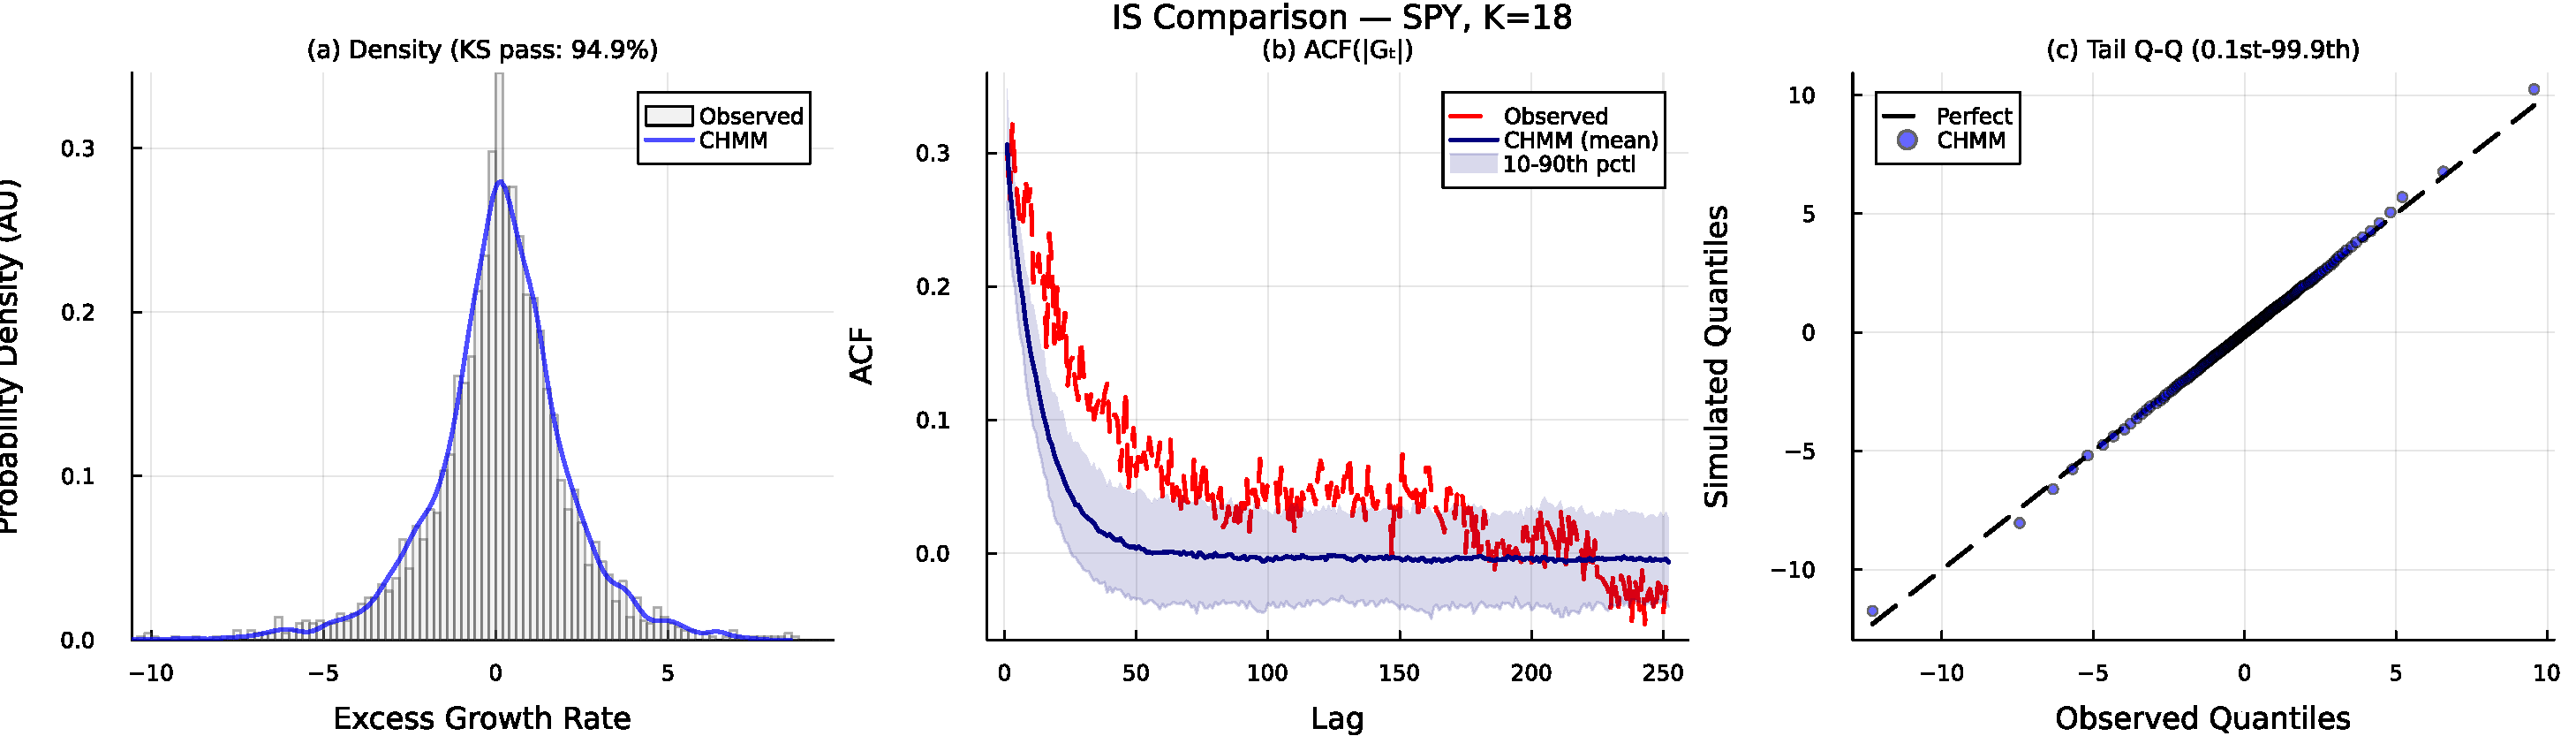
\includegraphics[width=\textwidth]{figs/Fig-3-IS-Comparison-K18.pdf}
\caption{\textbf{IS CHMM-N validation on SPY} ($K = 18$, $1{,}000$ simulated paths). Panel~(a): marginal density of the annualized excess log return $G_t$; gray histogram $=$ observed IS series, blue curve $=$ one simulated path. Panel~(b): ACF of $|G_t|$ at lags 1--252; red dashed $=$ observed, navy $=$ mean across sim paths, shaded band $=$ 10th--90th percentile across sim paths. Panel~(c): tail Q-Q plot at $200$ quantile levels; blue points $=$ simulated pooled over paths, black dashed $=$ identity.}
\label{fig:is_comparison}
\end{figure}

\subsection{Cross-Ticker Generalization (Pipeline~A)}
\label{sec:cross_asset_univariate}

Still under Pipeline~A: each ticker is fit independently, no cross-asset coupling.
Table~\ref{tab:cross_ticker} reports CHMM-t IS and OoS KS pass rates across the five additional tickers (NVDA, JNJ, JPM, AAPL, QQQ), each fit independently at $K = 18$. CHMM-t is the natural generalization vehicle here because it carries the strongest OoS KS in the SPY headline panel ($85.9\%$, against $84.2\%$ for CHMM-N and $79.3\%$ for CHMM-L) and supplies the per-state heavy tails that the outlier-prone single-name tickers (NVDA, JNJ) require. Per-family $K$-sensitivity for SPY across all three emission variants and per-ticker price-level metrics across all three families are in Appendix~\ref{sec:supplementary}.
The univariate fidelity persists across the panel on IS KS ($95.2\%$ to $99.8\%$). On OoS, JNJ, AAPL, and QQQ generalise cleanly ($90$--$95\%$), while NVDA ($57.2\%$) and JPM ($53.0\%$) show substantial OoS degradation, a stationarity artefact: the IS-fixed transitions and emissions cannot capture the AI-driven NVDA regime or the rate-repricing cycle for financials in the $2024$--$2026$ holdout.
A walk-forward quarterly refit recovers $\sim 15$ percentage points of the JPM gap (Appendix~\ref{sec:supplementary}); we acknowledge the residual cliff as a stationarity-scope limitation rather than a model-selection issue (it persists at every $K$ in the sweep).

\begin{table}[t]
\centering
\caption{\textbf{Cross-ticker generalization, CHMM-t at $K = 18$}. Each ticker fit independently; $1{,}000$ simulated paths, $\alpha = 0.05$. Observed kurtosis is the IS sample value.}
\label{tab:cross_ticker}
\small
\begin{tabular}{l cc c c c}
\toprule
& \multicolumn{2}{c}{KS (\%) $\uparrow$} & \multicolumn{2}{c}{Kurtosis} & ACF-MAE \\
\cmidrule(lr){2-3} \cmidrule(lr){4-5}
Ticker & IS & OoS & Obs & Sim & $\downarrow$ \\
\midrule
SPY  & $95.2$ & $84.1$ & $7.7$ & $14.68$ & $0.0551$ \\
NVDA & $99.1$ & $57.2$ & $5.5$ & $46.40$ & $0.0478$ \\
JNJ  & $99.8$ & $94.3$ & $9.0$ & $99.66$ & $0.0332$ \\
JPM  & $99.2$ & $53.0$ & $7.6$ & $18.82$ & $0.0483$ \\
AAPL & $99.1$ & $94.7$ & $3.2$ & $7.54$  & $0.0424$ \\
QQQ  & $96.1$ & $90.3$ & $3.4$ & $3.30$  & $0.0576$ \\
\bottomrule
\end{tabular}
\end{table}

\subsection{Rolling-Origin Out-of-Sample (Pipeline~A)}
\label{sec:rolling_origin}

Still under Pipeline~A: only the IS / OoS fit window rolls forward, no cross-asset coupling is introduced.
The single $2024$--$2026$ OoS window above is qualified by a five-window rolling-origin evaluation (eight-year IS, one-year OoS, sliding through $2022$--$2026$) at $\alpha = 0.05$ on the unconditional Kupiec test.
The $2022$ window is a structural counter-example: the rate-hike cycle is not represented in the preceding eight years of near-zero rates, OoS KS collapses to $0.2$--$0.4\%$, and Kupiec rejects with $\text{LR}_{\text{uc}}^{5\%} = 31.6$--$41.4$.
The $2024$, $2025$, and $2026$-year-to-date windows all pass Kupiec at $5\%$ cleanly with OoS KS in the $87$--$97\%$ range, and the $2023$ window is intermediate.
Excluding the $2022$ structural-break window, CHMM-t IS KS is $95.8\% \pm 1.6\%$ and OoS KS is $91.1\% \pm 3.5\%$.
The headline single-window result is closer to the modal behaviour than to the worst case, and the $2022$ window is the most informative single piece of negative evidence on the stationarity scope: the CHMM scaffold is well-calibrated when the IS window contains volatility regimes comparable to those of the OoS window, and fails predictably under structural breaks that lie outside the IS support. A rolling refit of $\hat{\mathbf{T}}$ and the emissions each quarter is the natural operational remedy.

\begin{figure}[t]
\centering
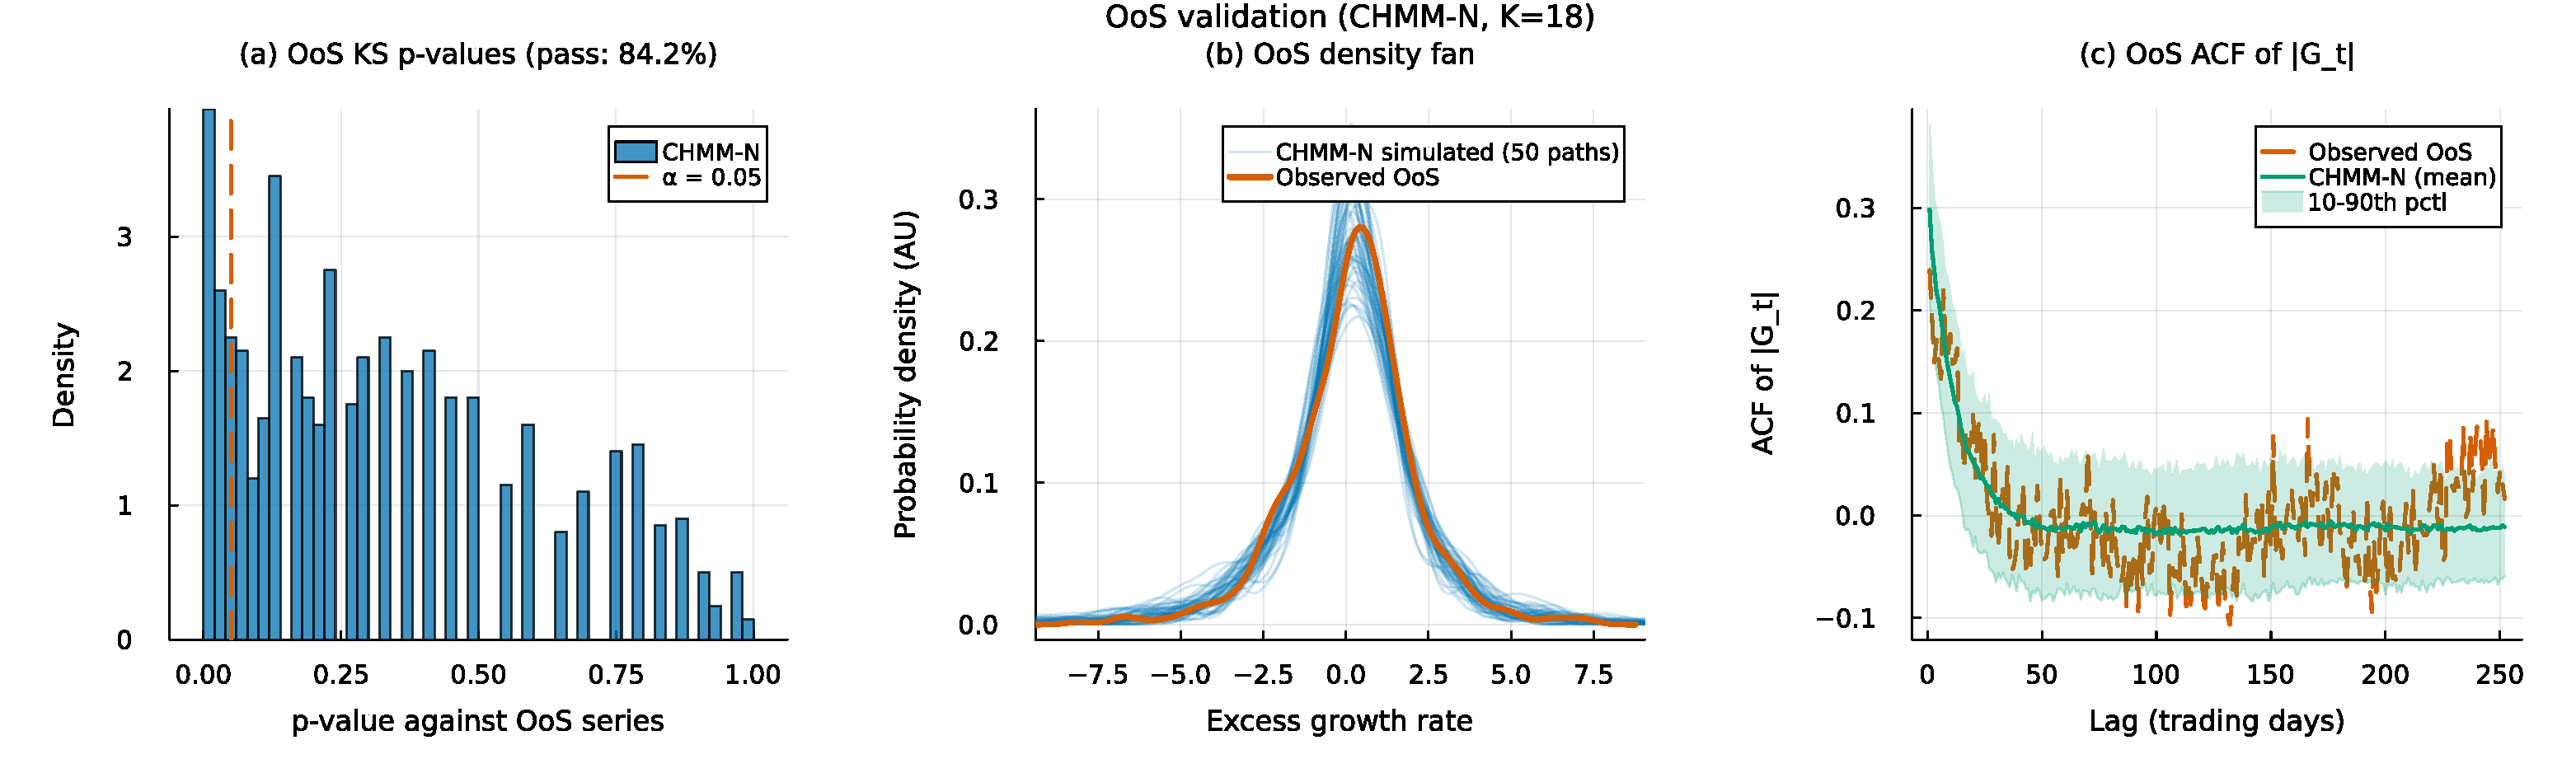
\includegraphics[width=\textwidth]{figs/Fig-4-OoS-Validation-K18.pdf}
\caption{\textbf{OoS CHMM-N validation on SPY} ($K = 18$, $1{,}000$ paths, $T_{\text{OoS}} = 572$). Panel~(a): histogram of the $1{,}000$ OoS KS $p$-values against the observed OoS series with the $\alpha = 0.05$ threshold (red dashed). Panel~(b): OoS return-density fan; blue thin curves $=$ simulated densities, red thick curve $=$ observed OoS density. Panel~(c): ACF of $|G_t|$ on the OoS window; red dashed $=$ observed, navy $=$ mean across sim paths, shaded band $=$ 10th--90th percentile.}
\label{fig:oos_validation}
\end{figure}

\subsection{Cross-Asset Dependence (Pipeline~B): Student-t Copula}
\label{sec:cross_asset}

This subsection is the only Pipeline~B subsection in the main text (Figure~\ref{fig:pipeline_schematic}, bottom row): we reuse the per-asset CHMM-N marginals from the Pipeline-A fits of Section~\ref{sec:cross_asset_univariate} and add a cross-asset dependence layer on top.
For multi-asset synthesis we inject cross-sectional dependence through the rank-based Student-t copula of Section~\ref{sec:cross_asset_methods}, the strongest dependence layer in our larger panel; the SIM and Gaussian copula constructions are reported in Appendix~\ref{sec:supplementary}.
The per-asset marginals here are the CHMM-N fits at $K = 18$; rank reordering preserves whichever marginal it receives exactly (Proposition~\ref{prop:rank_marginals}), so the dependence-layer ranking is invariant to the choice of CHMM emission family, and the Pipeline-B numbers below transfer unchanged to CHMM-t or CHMM-L marginals up to the per-asset KS sanity-check column.
Profile maximum likelihood over $\nu \in \{2, 3, 4, 5, 6, 8, 10, 15, 20, 30\}$ on the six-asset universe (SPY, NVDA, JNJ, JPM, AAPL, QQQ; $T = 2{,}516$ IS, $200$ simulated paths) selects $\nu^\star = 6$, consistent with values typically reported for equity indices \citep{demarta2005tcopula, mcneil2015quantitative}.

\begin{table}[t]
\centering
\caption{\textbf{Cross-asset Student-t copula on CHMM-N marginals} (Pipeline~B; $\nu^\star = 6$ by profile MLE; $200$ paths). Per-asset KS pass rate at $\alpha = 0.05$ (rank reordering preserves marginals exactly, so the per-asset KS column is a sanity check after dependence injection rather than a substitute for Table~\ref{tab:cross_ticker}). The lower block reports correlation reproduction averaged over paths: Frobenius norm of $\hat\Sigma_{\text{sim}} - \hat\Sigma_{\text{obs}}$ and off-diagonal mean absolute error. Comparison against SIM and the Gaussian copula on the same marginals is in Appendix~\ref{sec:supplementary}; the Student-t copula is the best of the three on every metric (off-diagonal MAE $0.027$ vs.\ $0.031$ Gaussian, $0.076$ SIM).}
\label{tab:cross_asset}
\small
\begin{tabular}{l cc}
\toprule
& \multicolumn{2}{c}{KS (\%) $\uparrow$} \\
\cmidrule(lr){2-3}
Ticker & IS & OoS \\
\midrule
SPY   & $95.5$  & $86.0$ \\
NVDA  & $93.0$  & $50.5$ \\
JNJ   & $100.0$ & $93.5$ \\
JPM   & $96.5$  & $49.0$ \\
AAPL  & $99.0$  & $94.5$ \\
QQQ   & $93.0$  & $95.0$ \\
\midrule
Mean   & $96.2$ & $78.1$ \\
Median & $96.0$ & $89.8$ \\
\midrule
\multicolumn{3}{l}{\textit{Correlation reproduction (averaged over $200$ paths)}} \\
Frobenius IS         & \multicolumn{2}{c}{$0.184$} \\
Off-diag MAE IS      & \multicolumn{2}{c}{$0.027$} \\
Frobenius OoS        & \multicolumn{2}{c}{$1.499$} \\
Off-diag MAE OoS     & \multicolumn{2}{c}{$0.208$} \\
\bottomrule
\end{tabular}
\end{table}

The Student-t copula preserves each asset's fitted CHMM marginal exactly by the rank-reordering construction, so the per-asset KS column (median $96.0\%$ IS, $89.8\%$ OoS) is a sanity check on the copula sample rather than a substitute for Table~\ref{tab:cross_ticker}.
The central dependence-layer claim is the off-diagonal correlation MAE: $0.027$ on IS, against $0.031$ for the Gaussian copula and $0.076$ for the SIM factor baseline on the same marginals (Appendix~\ref{sec:supplementary}).
The copula advantage is intrinsic to the rank-reordering construction rather than specific to the marginal model.

\subsection{Value-at-Risk and Expected-Shortfall Back-Test (Pipeline~A)}
\label{sec:var_backtest}
\label{sec:utility}

Still under Pipeline~A (Figure~\ref{fig:pipeline_schematic}): VaR and Expected-Shortfall are evaluated on the per-ticker SPY simulations, no cross-asset coupling.
For a financial-risk consumer the canonical diagnostics are one-tail Value-at-Risk (VaR) and Expected-Shortfall (ES) at daily probability levels of $1\%$ and $5\%$.
A synthetic-data generator is well calibrated if the envelope of per-path simulated VaR/ES brackets the observed historical value.
We simulate $1{,}000$ independent paths from each of the six most relevant generators (Bootstrap, GARCH(1,1), CHMM-N, CHMM-t, CHMM-L, CHMM-GED) and report median and $[5\%, 95\%]$ envelope across paths in Table~\ref{tab:var_es}.

\begin{table}[t]
\centering
\caption{\textbf{VaR and Expected-Shortfall envelope for SPY} ($N_{\text{paths}} = 1{,}000$). Each entry is the median and $[5\%, 95\%]$ envelope across paths of the left-tail VaR / ES at $\alpha \in \{0.01, 0.05\}$; observed historical values are in the first row. All four CHMM variants bracket the observed historical VaR and ES at both levels on both windows. Note on the repeated $\text{LR}_{\text{uc}} = 3.83$ values across CHMM rows in the body discussion: the unconditional Kupiec statistic at $T = 572$ trading days and $p = 0.05$ takes integer-breach-count values (e.g., $k = 19$ breaches gives $\text{LR}_{\text{uc}} = 3.828$, just below the asymptotic $\chi^2_1$ critical value of $3.841$); the apparent agreement across rows reflects the coarse integer-breach grid at this $T_{\text{OoS}}$, not a numerical coincidence in the underlying simulated samples.}
\label{tab:var_es}
\small
\resizebox{\textwidth}{!}{%
\begin{tabular}{l l l l l}
\toprule
          & IS VaR$_{0.01}$              & IS ES$_{0.01}$               & IS VaR$_{0.05}$              & IS ES$_{0.05}$               \\
Model     & median $[5\%, 95\%]$         & median $[5\%, 95\%]$         & median $[5\%, 95\%]$         & median $[5\%, 95\%]$         \\
\midrule
\textit{Observed}  & $-6.38$                      & $-9.00$                      & $-3.43$                      & $-5.50$                      \\
Bootstrap & $-6.38\ [-7.04, -5.99]$      & $-8.86\ [-10.37,\ -7.78]$    & $-3.43\ [-3.68, -3.20]$      & $-5.46\ [-5.99, -5.05]$      \\
GARCH     & $-5.80\ [-8.62, -4.52]$      & $-7.86\ [-13.54,\ -5.77]$    & $-3.19\ [-3.92, -2.71]$      & $-4.89\ [-7.11, -3.91]$      \\
CHMM-N    & $-6.64\ [-8.01, -5.47]$      & $-8.80\ [-10.16,\ -7.34]$    & $-3.45\ [-4.05, -2.95]$      & $-5.45\ [-6.33, -4.61]$      \\
CHMM-t    & $-6.58\ [-7.51, -5.83]$      & $-9.06\ [-10.70,\ -7.79]$    & $-3.40\ [-3.90, -2.90]$      & $-5.51\ [-6.18, -4.85]$      \\
CHMM-L    & $-6.89\ [-7.85, -6.01]$      & $-9.15\ [-10.42,\ -7.97]$    & $-3.30\ [-3.77, -2.88]$      & $-5.53\ [-6.17, -4.87]$      \\
CHMM-GED  & $-6.85\ [-7.70, -6.06]$      & $-8.79\ [-9.83,\ -7.82]$     & $-3.43\ [-3.98, -2.93]$      & $-5.55\ [-6.23, -4.91]$      \\
\midrule
          & OoS VaR$_{0.01}$             & OoS ES$_{0.01}$              & OoS VaR$_{0.05}$             & OoS ES$_{0.05}$              \\
\textit{Observed}  & $-5.51$                      & $-7.94$                      & $-2.77$                      & $-4.67$                      \\
Bootstrap & $-6.33\ [-7.60, -5.28]$      & $-8.43\ [-11.76,\ -6.59]$    & $-3.39\ [-3.91, -2.88]$      & $-5.34\ [-6.38, -4.50]$      \\
GARCH     & $-5.35\ [-9.98, -3.61]$      & $-6.72\ [-13.51,\ -4.38]$    & $-3.14\ [-4.94, -2.36]$      & $-4.59\ [-7.92, -3.23]$      \\
CHMM-N    & $-6.30\ [-9.02, -4.30]$      & $-8.44\ [-11.36,\ -5.42]$    & $-3.39\ [-4.74, -2.47]$      & $-5.27\ [-7.23, -3.74]$      \\
CHMM-t    & $-6.32\ [-8.13, -4.80]$      & $-8.60\ [-12.20,\ -6.29]$    & $-3.29\ [-4.27, -2.45]$      & $-5.34\ [-6.72, -4.08]$      \\
CHMM-L    & $-6.69\ [-8.59, -4.91]$      & $-8.88\ [-11.48,\ -6.73]$    & $-3.27\ [-4.30, -2.51]$      & $-5.47\ [-6.82, -4.20]$      \\
CHMM-GED  & $-6.60\ [-8.30, -4.82]$      & $-8.51\ [-10.68,\ -6.47]$    & $-3.32\ [-4.38, -2.46]$      & $-5.41\ [-6.66, -4.06]$      \\
\bottomrule
\end{tabular}%
}
\end{table}

All four CHMM variants bracket the observed historical VaR and ES at both $1\%$ and $5\%$ levels within their $5\%$--$95\%$ envelopes on both IS and OoS windows; the IS CHMM-N median VaR$_{0.01}$ at $-6.64$ (observed $-6.38$) and ES$_{0.01}$ at $-8.80$ (observed $-9.00$) are the closest point estimates across the six generators.
The CHMM envelopes are roughly $1.7\times$ tighter than GARCH's and pass the unconditional Kupiec test cleanly at both levels (CHMM-N $\text{LR}_{\text{uc}} = 3.83$ at $5\%$ against the $\chi^2_1 = 3.84$ critical value; CHMM-t at $3.83$; CHMM-L at $3.03$; CHMM-GED at $3.83$).
CHMM-t's IS kurtosis overshoot does \emph{not} translate into a systematically more conservative VaR/ES point estimate; the IS median VaR$_{0.01}$ of $-6.58$ is almost identical to CHMM-N's $-6.64$ and the envelope width is comparable. CHMM-L's IS median VaR$_{0.01}$ of $-6.89$ is mildly more conservative than CHMM-N's, consistent with its closer-to-observed kurtosis. CHMM-GED's IS median VaR$_{0.01}$ of $-6.85$ sits between CHMM-N and CHMM-L on the conservativeness axis, consistent with its adaptive shape mechanism.

\paragraph{Conditional coverage (Christoffersen 1998).}
The Kupiec statistic only checks the unconditional breach rate. We complement it with the Christoffersen \cite{christoffersen1998evaluating} independence ($\text{LR}_{\text{ind}}$, $\sim\chi^2_1$) and joint conditional-coverage ($\text{LR}_{\text{cc}} = \text{LR}_{\text{uc}} + \text{LR}_{\text{ind}}$, $\sim\chi^2_2$) tests. We report two variants: the unconditional pooled-archive variant matched to the rest of the body panel, and a regime-conditional variant that propagates the latent-state forecast $\Prob(s_{t+1}\,|\,\mathcal F_t)$ through the CHMM emission mixture under IS-fixed parameters. Every unconditional generator in the panel (i.i.d.\ bootstrap, GARCH(1,1), and all four CHMM variants) rejects independence on the OoS window at $\alpha = 0.05$ for both VaR levels (CHMM-N at $5\%$: $\text{LR}_{\text{ind}} = 5.26$, $p = 0.022$; $\text{LR}_{\text{cc}} = 9.08$, $p = 0.011$; full unconditional panel in Appendix~\ref{sec:christoffersen_supp}, Table~\ref{tab:christoffersen_var}). The independence rejection is driven by volatility-clustering in $R_{\text{oos}}$ that any unconditional generator with a constant-across-$t$ VaR threshold is structurally unable to track. The regime-conditional variant addresses this directly: at each OoS day $t$, we run the forward filter through $\mathcal F_{t-1} = R_{\text{IS}} \cup R_{\text{oos}}[1{:}t-1]$ to get the one-step-ahead state forecast $\Prob(s_t = k \mid \mathcal F_{t-1}) = \sum_i \Prob(s_{t-1} = i \mid \mathcal F_{t-1}) \cdot T_{ik}$ and define $\widehat{\text{VaR}}_t(\alpha) = F_t^{-1}(\alpha)$ where $F_t$ is the $K$-component Gaussian-mixture predictive CDF $\sum_k \Prob(s_t = k \mid \mathcal F_{t-1}) \cdot \Phi(\,\cdot\,;\, \mu_k, \sigma_k)$. Table~\ref{tab:cond_var} reports the resulting back-test for CHMM-N at $K^\star = 3$ and at $K = 18$ on the OoS window.

\begin{table}[h]
\centering
\small
\caption{\textbf{Regime-conditional VaR back-test for CHMM-N on the OoS window} ($T_{\text{oos}} = 572$ days, seed $= 20260420$). At each $t$, conditional VaR is the $\alpha$-quantile of the one-step-ahead Gaussian-mixture predictive density under IS-fixed parameters. Critical values: $\chi^2_1(0.05) = 3.841$, $\chi^2_2(0.05) = 5.991$. Every $(K, \alpha)$ row passes Kupiec, Christoffersen-ind, and Christoffersen-cc cleanly at $\alpha = 0.05$, in contrast to the unconditional pooled-archive variant which rejects independence at every CHMM, GARCH, and bootstrap row on OoS (Table~\ref{tab:christoffersen_var}).}
\label{tab:cond_var}
\begin{tabular}{c c c c c c c c c c}
\toprule
$K$ & $\alpha$ & breaches & br rate & med VaR & $\text{LR}_{\text{uc}}$ & $p_{\text{uc}}$ & $\text{LR}_{\text{ind}}$ & $\text{LR}_{\text{cc}}$ & $p_{\text{cc}}$ \\
\midrule
$3$  & $0.01$ & $9$  & $1.57\%$ & $-4.56$ & $1.62$ & $0.20$ & $2.36$ & $3.98$ & $0.14$ \\
$3$  & $0.05$ & $35$ & $6.12\%$ & $-2.87$ & $1.41$ & $0.24$ & $0.01$ & $1.42$ & $0.49$ \\
$18$ & $0.01$ & $9$  & $1.57\%$ & $-5.20$ & $1.62$ & $0.20$ & $2.36$ & $3.98$ & $0.14$ \\
$18$ & $0.05$ & $26$ & $4.55\%$ & $-3.02$ & $0.26$ & $0.61$ & $0.52$ & $0.78$ & $0.68$ \\
\bottomrule
\end{tabular}
\end{table}

The conditional-VaR construction passes all three tests at every $(K, \alpha)$ on OoS, with breach rates of $1.57\%$ and $4.55$--$6.12\%$ against nominal $1\%$ and $5\%$. The independence-test improvement from the unconditional variant ($\text{LR}_{\text{ind}} = 5.26$ at $K = 18$, $\alpha = 0.05$) to the conditional variant ($\text{LR}_{\text{ind}} = 0.52$) is the regime-switching value proposition that the Kupiec-only headline did not exercise: the latent-state forecast tightens the threshold in clustered-volatility windows so that breaches do not pile up at sub-runs of high volatility. The same construction does not require retuning $K$ on a stress-test slice nor a different parameter family for VaR consumers; it reuses the IS-fixed CHMM-N transitions and emissions and runs the forward filter on the OoS series under those frozen parameters. The full unconditional Christoffersen panel across the six panel rows (Bootstrap, GARCH, CHMM-N/-t/-L/-GED) is in Appendix~\ref{sec:christoffersen_supp}.


\section{Discussion}
\label{sec:discussion}
The main empirical finding is that a continuous HMM trained by Baum-Welch with quantile-based initialisation reproduces the three symmetric Cont stylized facts on daily US equity returns at the body operating point $K^\star = 3$ and closes the kurtosis gap to within the heavy-tailed-emission family choice. Two issues compound in the \citet{ryden1998stylized} low-$K$ setup: a single self-transition rate produces a single exponential mode, and 1990s-standard random initialisations often converged to degenerate local optima. Our $K = 2$ replication on SPY confirmed the binding constraint is distributional (KS at $K = 2$ dropped to $67$ to $72\%$, while ACF-MAE was essentially constant at approximately $0.050$; full panel in the appendix, Section~\ref{sec:ryden_replication}); with modern initialisation the ACF was reproduced at any $K \ge 2$ and distributional fidelity drove the choice of $K$. The mechanistic source of the residual kurtosis gap is that CHMM-N at $K^\star = 3$ produced simulated IS kurtosis $3.83$ against observed $7.68$ (Table~\ref{tab:model_comparison}) because a three-component Gaussian mixture's between-component term is bounded and cannot tile the empirical heavy tail. The shared-$\nu$ Student-$t$ ablation was the primary heavy-tailed specification at $K^\star = 3$ (simulated IS kurtosis $4.68$, no penalty hyperparameter; Table~\ref{tab:model_comparison}), the penalised per-state CHMM-t at $\lambda = 20$ overshot IS kurtosis to $14.91$ ($\lambda$ tuned at $K = 18$ and re-used at $K^\star = 3$ as an upper bound; Table~\ref{tab:model_comparison}), CHMM-L sat between CHMM-N and CHMM-t at IS kurtosis $5.30$ without any shape parameter (Table~\ref{tab:model_comparison}), and CHMM-GED's bimodal $\hat p_k$ partition was the data-driven analog of a hand-classified Gaussian-bulk with Laplace-tail hybrid. The mechanism is therefore that the binding axis at $K \ge 3$ is the marginal mixture's representational capacity for empirical kurtosis, not the temporal kernel; the emission-family ablation isolates which symmetric heavy-tail specification carries the residual gap most cleanly.

The honest limitation is that a static-IS-fit CHMM does not generalize across regime introductions. The GLD non-equity stress and the W2 (COVID) and W4 (2022 rate-hike onset) walk-forward folds were regime introductions that the IS distribution did not span, so OoS performance broke down on slices whose marginal moved outside the IS regime library (Table~\ref{tab:stationarity_scope}). Single-name equity returns are well known to carry sector-specific structural breaks~\cite{pastorstambaugh2001equity, andreoughysels2002breaks, angtimmermann2012regime}, and the cross-ticker concentration of failures on regime-introduction names (LLY, UNH, NEM) is the same pattern at the panel level. Periodic refit~\cite{pesarantimmermann2007window, cappe2011online} is the deployment recipe for non-stress equity slices; it does not save GLD or the W2 and W4 stress folds, which the IS distribution does not span and which faster refit cadences also do not close. The identifiability implication is that the binding axis for $K$-selection is distributional rather than temporal: the ACF was reproduced at any $K \ge 2$ once initialisation was fixed, so held-out KS, log-likelihood, and BIC are the load-bearing criteria for $K^\star$ selection, and the stress-fold rejections are diagnostic of OoS-slice composition rather than of model misspecification on the IS axis.

The generalizability story is bounded by both the stylized-fact scope and the parameter-parsimony comparison against deeper baselines. The Cont (2001) stylized-fact list also includes the leverage effect (negative $\mathrm{Corr}(G_t, |G_{t+1}|)$ on equity returns); the present paper's body evaluation covered only the three symmetric stylized facts and treats the leverage-axis behaviour of symmetric-emission CHMMs as a deferred topic. On parametric complexity, CHMM-N at $K = 18$ has $K(K-1) + 2K = 342$ free parameters (CHMM-t adds $K$ degrees of freedom; CHMM-GED adds $K$ shape parameters), whereas the QuantGAN baseline of \citet{wiese2020quantgan} carries on the order of $10^4$ to $10^5$ parameters across its convolutional generator and critic, three orders of magnitude higher; the CHMM therefore competes against deep generators at a parameter budget that is amenable to identifiability analysis, posterior diagnostics, and the closed-form spectral mechanism that motivates the $K^\star$ choice. The architectural counterpoint to that parsimony is that asymmetric or skewed emission families, a time-varying transition kernel estimated by rolling refit or online updates, scaling the multi-asset copula composition beyond the six-asset and 30-ticker panels through factor or vine structures, and embedding the CHMM-mixed predictive in a portfolio-optimisation or tail-risk-budgeting loop are the natural future directions; each would extend the present construction on a single orthogonal axis (leverage effect, non-stationarity, dimension, downstream use case) without disturbing the unified four-family scaffold that the body of this paper exercises.


\section{Conclusion}
\label{sec:conclusion}
A continuous HMM trained by Baum-Welch with quantile-based initialization reproduces the three symmetric Cont stylized facts on daily US-equity returns. The textbook mixture-of-eigenvalues identity for the absolute-return ACF (\citealp{hamilton1994time, krolzig1997markov, timmermann2000moments}) recasts the \citet{ryden1998stylized} low-$K$ failure as an effective-rank statement on $\mathbf T - \mathbf 1\bar{\boldsymbol\pi}^\top$, non-binding at the cross-ticker median for $K \ge 3$. A regime-conditional Value-at-Risk across four emission families passes Christoffersen-cc at $\alpha = 0.05$ on the headline OoS window and on $19/24$ walk-forward rows, with strict-tail DQ behaviour favouring CHMM-N at $K^\star = 3$ over filtered-bootstrap and CAViaR contenders. ML HSMM-N at $K^\star = 3$ ($91.0\%$ OoS KS) is the strongest single-window parametric row; scope is daily US equities under stationary OoS (Table~\ref{tab:stationarity_scope}).

\paragraph{Author Contributions and Data Availability.}
J.V.\ directed the study. A.A.\ developed the continuous model and simulation code, implemented Baum-Welch, conducted the in-sample and out-of-sample analysis, and generated all figures and tables. C.J.\ contributed to ECM-derivation methodology review and to validation of the cross-decade and cross-ticker pipelines. All authors edited the final manuscript. The authors declare no conflict of interest. Reproducer: \url{https://github.com/altashly1/CHMM-paper}; companion Julia package \texttt{CHMM-Model.jl}: \url{https://github.com/altashly1/CHMM-Model} (MIT). Daily prices: Polygon.io via Massive (2014-01-03 to 2025-11-18) and Alpaca / IEX (extension through 2026-04-20).


% ========================================================================================= %
\bibliographystyle{unsrtnat}
\bibliography{references}

% ========================================================================================= %
\appendix

\section{Supplementary Material}
\label{sec:supplementary}
This appendix collects supplementary material referenced in the main body: the public API of the companion package, the EM forward-backward recursions and algorithm pseudocode, the validation metric definitions, formal propositions, the full state-resolution and multi-emission sensitivity panels, robustness and KS-power calibration, the extended GARCH and SM-CHMM baselines, the full cross-asset panel, and the $K$-selection and $\nu_k$ diagnostics referenced from the discussion.

\subsection{CHMM-Model.jl Public API and Reproducer}
\label{sec:supp_chmm_api}

The companion Julia package \texttt{CHMM-Model.jl} (\url{https://github.com/altashly1/CHMM-Model}) is the entry point used to regenerate every table and figure in this paper from a single seed root under Julia $\geq 1.12$. The public surface is a single \texttt{CHMM} type, three emission constructors, a unified \texttt{fit!} method (log-space Baum-Welch / ECM), and a unified \texttt{simulate} method.

\begin{verbatim}
using CHMM
chmm_n = make_chmm_n(returns; K = 18)        # Gaussian emissions
chmm_t = make_chmm_t(returns; K = 18)        # Student-t emissions
chmm_l = make_chmm_l(returns; K = 18)        # Laplace emissions
fit!(chmm_n; max_iter = 60, tol = 1e-4)      # log-space Baum-Welch
paths = simulate(chmm_n; T = 2516, n = 1000) # 1000 paths of length T
\end{verbatim}

The same \texttt{simulate} interface is used for every benchmark generator (Bootstrap, Gaussian i.i.d., Laplace i.i.d., GARCH(1,1)) so that the seven-metric panel evaluates each row on byte-identical windows. The Pipeline~B Student-t copula sampler is exposed as \texttt{simulate\_copula(\dots; nu = 6)} on the per-asset CHMM marginals; the rank-reordering construction is one function call. Running \texttt{julia --project=. run\_full\_rebuild.jl} from the paper repository (\url{https://github.com/altashly1/CHMM-paper}) reproduces every numerical artifact under the global seed policy of Section~\ref{sec:metrics}; \texttt{Manifest.toml} pins the dependency graph.

\subsection{CHMM Algorithms and Derivations}
\label{sec:supp_algorithms}
\paragraph{Forward-backward recursions and M-step updates.}
For reference, the Baum-Welch description in the main text is underpinned by the standard log-space recursions~\cite{rabiner1986introduction, bilmes1998gentle}.
Define the forward variable $\alpha_t(k) = \Prob(O_{1:t}, S_t = k \mid \mathcal{M})$ and the backward variable $\beta_t(k) = \Prob(O_{t+1:T} \mid S_t = k, \mathcal{M})$.
The log-space recursions are
\begin{align}
    \log \alpha_1(k) &= \log \pi_k + \log f_k(O_1), \label{eq:forward_init} \\
    \log \alpha_t(j) &= \underset{i}{\text{logsumexp}}\!\left(\log \alpha_{t-1}(i) + \log T_{ij}\right) + \log f_j(O_t), \quad t = 2, \ldots, T, \label{eq:forward} \\[4pt]
    \log \beta_T(k) &= 0, \label{eq:backward_init} \\
    \log \beta_t(i) &= \underset{j}{\text{logsumexp}}\!\left(\log T_{ij} + \log f_j(O_{t+1}) + \log \beta_{t+1}(j)\right), \quad t = T{-}1, \ldots, 1, \label{eq:backward}
\end{align}
where $\text{logsumexp}_i(x_i) = x_{\max} + \log \sum_i \exp(x_i - x_{\max})$.
The posterior state-occupancy $\gamma_t(k)$ and pair-occupancy $\xi_t(i, j)$ quantities are
\begin{equation}
    \gamma_t(k) = \frac{\alpha_t(k) \beta_t(k)}{\sum_j \alpha_t(j) \beta_t(j)}, \qquad
    \xi_t(i, j) = \frac{\alpha_t(i)\, T_{ij}\, f_j(O_{t+1})\, \beta_{t+1}(j)}{\sum_{m,n} \alpha_t(m)\, T_{mn}\, f_n(O_{t+1})\, \beta_{t+1}(n)},
    \label{eq:gamma_xi}
\end{equation}
and the closed-form M-step updates are
\begin{equation}
    \pi_k^{\text{new}} = \gamma_1(k),\quad
    \mu_k^{\text{new}} = \frac{\sum_t \gamma_t(k)\, O_t}{\sum_t \gamma_t(k)},\quad
    \left(\sigma_k^{\text{new}}\right)^2 = \frac{\sum_t \gamma_t(k)(O_t - \mu_k^{\text{new}})^2}{\sum_t \gamma_t(k)},\quad
    T_{ij}^{\text{new}} = \frac{\sum_{t=1}^{T-1} \xi_t(i, j)}{\sum_{t=1}^{T-1} \gamma_t(i)}.
    \label{eq:mstep}
\end{equation}
The convergence criterion is $|\mathcal{L}^{(n)} - \mathcal{L}^{(n-1)}| < \epsilon$ with $\epsilon = 10^{-4}$, where $\mathcal{L}^{(n)} = \text{logsumexp}_k \log \alpha_T(k)$ is the standard Baum-Welch observed-data log-likelihood of the parameters entering iteration $n$, evaluated by that iteration's forward pass \emph{before} any M-step can mutate them; the check runs before the update, so the returned parameters are always an evaluated iterate with a matching smoothed posterior, and the loop makes one final evaluation-only pass so that the last M-step update is itself scored. For the exact Gaussian and Laplace conditional maximisations the likelihood is monotone across iterations and the last evaluated iterate is returned; for the Student-$t$ and GED numerical block updates ascent is not guaranteed, the trace is monitored instead (see the numerical-optimisation scope paragraph of the supplementary propositions), and the best evaluated finite iterate $\arg\max_n \mathcal{L}^{(n)}$ is returned. Implementation note on $\boldsymbol\pi$: the Gaussian fitter departs from Eq.~\eqref{eq:mstep} in one place, holding $\boldsymbol\pi$ fixed at its uniform initial value instead of applying $\pi_k^{\text{new}} = \gamma_1(k)$; the Student-$t$, Laplace, and GED fitters apply the $\gamma_1$ update. Parameter counts and BIC penalties for CHMM-N accordingly exclude $\boldsymbol\pi$. Simulation draws $S_1$ from the stationary distribution $\bar{\boldsymbol\pi}$ of $\hat{\mathbf T}$ and then iterates $G_t \sim \mathcal{N}(\mu_{S_t}, \sigma_{S_t}^2)$, $S_{t+1} \sim \text{Categorical}(\mathbf{T}_{S_t, \cdot})$ with no jump process.

\paragraph{CHMM-t M-step (per-state ECM/ECME, closed form given $u_{t,k}$).}
For Student-t emissions $f_k(x) = t_{\nu_k}(x; \mu_k, \sigma_k)$ the ECM formulation of \citet{peel2000robust, liu1995ml} treats the latent precision as an augmented E-step quantity,
\begin{equation}
    u_{t,k} = \frac{\nu_k + 1}{\nu_k + ((O_t - \mu_k)/\sigma_k)^2},
    \label{eq:tprecision_supp}
\end{equation}
so that conditional on $\nu_k$ the location and scale admit closed-form weighted updates,
\begin{equation}
    \mu_k^{\text{new}} = \frac{\sum_t \gamma_t(k)\, u_{t,k}\, O_t}{\sum_t \gamma_t(k)\, u_{t,k}},\quad
    \left(\sigma_k^{\text{new}}\right)^2 = \frac{\sum_t \gamma_t(k)\, u_{t,k}\, (O_t - \mu_k^{\text{new}})^2}{\sum_t \gamma_t(k)}.
    \label{eq:tupdate_supp}
\end{equation}
The degrees-of-freedom parameter $\nu_k$ is then refined by a 40-iteration one-dimensional golden-section search on the per-state posterior-weighted objective $Q_k(\nu) = \sum_t \gamma_t(k)\, \log t_\nu(O_t; \mu_k, \sigma_k)$ over the bracket $(\nu_{\min}, \nu_{\max}) = (2.1, 50)$, with the smoothed posteriors $\gamma$ held fixed. Maximising this marginal state-weighted log-likelihood for $\nu_k$, rather than the augmented-data $u$-functional, follows the spirit of the ECME construction of \citet{liu1995ml}; in their single-component i.i.d.\ setting, where all $\gamma_t(k) = 1$, that objective is the observed-data likelihood, whereas already for i.i.d.\ mixtures the posterior-weighted objective differs from the observed-data likelihood \citep{peel2000robust}, and in the HMM the observed-data likelihood also depends on $\nu_k$ through the forward recursion, so this update is a hybrid generalised block-coordinate step on a surrogate objective and does not inherit the ECME observed-data ascent guarantee. We diagnose convergence from the observed-data log-likelihood trace rather than assert monotonicity, returning the best evaluated finite iterate (which is also restored if an update degenerates to a non-finite likelihood).
We extend this M-step with an optional exponential shrinkage prior on $1/\nu_k$, corresponding to the penalised objective
\begin{equation}
    Q_k^{\text{pen}}(\nu) \;=\; \sum_t \gamma_t(k)\, \log t_\nu(O_t; \mu_k, \sigma_k) \;-\; \lambda \, / \, \nu,
    \label{eq:nu_pen}
\end{equation}
maximised by the same golden-section search ($\lambda = 0$ recovers the unpenalised \citet{peel2000robust, liu1995ml}-style $\nu$ update; the rate sweep and its effect on simulated IS excess kurtosis are reported in the $K$-selection and $\nu_k$ diagnostics appendix, Table~\ref{tab:nu_shrinkage}).

\paragraph{CHMM-L M-step (closed-form weighted Laplace MLE).}
For Laplace emissions $f_k(x) = \tfrac{1}{2 b_k} \exp(-|x - \mu_k|/b_k)$, with the per-state Laplace scale denoted $b_k$ to avoid collision with the backward variable $\beta_t$, the weighted-MLE estimators are available in closed form:
\begin{equation}
    \mu_k^{\text{new}} = \text{WeightedMedian}\!\left(O_{1:T};\, \gamma_{1:T}(k)\right),\qquad
    b_k^{\text{new}} = \frac{\sum_t \gamma_t(k)\, |O_t - \mu_k^{\text{new}}|}{\sum_t \gamma_t(k)}.
    \label{eq:lupdate_supp}
\end{equation}
The weighted median is the first order statistic whose cumulative posterior weight reaches half the total, the minimiser of the weighted $L^1$ objective $\sum_t \gamma_t(k)\,|O_t - \mu|$; when the half-weight falls exactly between two adjacent order statistics, every point in the closed interval between them is a minimiser.
The Laplace M-step carries no shape parameter, so CHMM-L is strictly cheaper per iteration than CHMM-t (which requires the per-state $Q_k$ search).

\paragraph{CHMM-GED M-step (three-stage ECM-style update with closed-form scale).}
For Generalized Error Distribution emissions $f_k(x) = \mathrm{GED}(x; \mu_k, \alpha_k, p_k) = \frac{p_k}{2 \alpha_k \Gamma(1/p_k)} \exp\!\big(-(|x - \mu_k|/\alpha_k)^{p_k}\big)$ the M-step decomposes into three block updates per state. Given current $(\mu_k^{(n)}, \alpha_k^{(n)}, p_k^{(n)})$, the first block updates the location by minimising the per-state weighted $L^{p_k}$ loss,
\begin{equation}
    \mu_k^{(n+1)} \;=\; \operatorname{GoldenSearchMin}_{\mu \in I_k} \;\sum_t \gamma_t(k)\, \big|O_t - \mu\big|^{p_k^{(n)}},
    \qquad I_k \;=\; \big[\min_t O_t,\, \max_t O_t\big],
    \label{eq:ged_mu}
\end{equation}
by a $40$-iteration golden-section search; CM-2 updates the scale in closed form given $(\mu_k^{(n+1)}, p_k^{(n)})$,
\begin{equation}
    \alpha_k^{(n+1)} \;=\; \left[\frac{p_k^{(n)}}{W_k} \sum_t \gamma_t(k)\, \big|O_t - \mu_k^{(n+1)}\big|^{p_k^{(n)}}\right]^{1 / p_k^{(n)}}, \qquad W_k \;=\; \sum_t \gamma_t(k);
    \label{eq:ged_alpha}
\end{equation}
and CM-3 updates the shape by maximising the per-state $Q$-function over the bracket,
\begin{equation}
    p_k^{(n+1)} \;=\; \operatorname{GoldenSearchMax}_{p \in [p_{\min},\, p_{\max}]} \;\sum_t \gamma_t(k)\, \log f_k\!\big(O_t;\, \mu_k^{(n+1)},\, \alpha_k^{(n+1)},\, p\big),
    \label{eq:ged_p}
\end{equation}
again by a $40$-iteration golden-section search over $[p_{\min}, p_{\max}] = [0.5, 3.0]$. The scale update is the exact conditional maximiser. The location objective is convex when $p_k \ge 1$ but can be nonconvex when $p_k < 1$, and both bracketed searches are finite numerical approximations. Accordingly, we use ``ECM-style'' for this three-block procedure and assess convergence from the observed-data log-likelihood trace; the exact ECM monotonicity result~\citep{mengrubin1993ecm} would require every block to attain a conditional maximum. At the boundary cases, $p_k = 2$ recovers Gaussian (with $\sigma = \alpha/\sqrt{2}$) and $p_k = 1$ recovers Laplace (with $b = \alpha$).

\paragraph{Algorithm descriptions.}
The unified EM procedure shared across all four emission families is given in Algorithm~\ref{alg:chmm_em}: a shared framework (quantile-based initialisation, log-space forward-backward, transition update) plus four family-specific branches at lines~\ref{line:init}, \ref{line:emit}, and \ref{line:mstep}. The simulator is given in Algorithm~\ref{alg:chmm_simulate}, and the cross-asset rank-reordering simulator for the multi-asset construction in Algorithm~\ref{alg:copula_sim}. Viterbi and SIM-resampling pseudocode are provided in the companion code repository; both are textbook constructions and we omit them from the appendix.

% ========================================================================================= %
% Algorithm 1: Baum-Welch (EM) for Continuous Gaussian HMM
% ========================================================================================= %
% Unified EM algorithm with family-specific M-step switch
% ========================================================================================= %
\begin{breakablealgorithm}
\caption{Unified EM algorithm for the CHMM family. Lines~\ref{line:init}, \ref{line:emit}, and \ref{line:mstep} branch on the emission family $F \in \{\mathcal{N}, t, L, \text{GED}\}$; every other line is identical across families. The CHMM-N and CHMM-L variants instantiate classical EM; CHMM-t and CHMM-GED use ECM-style block updates whose shape step is a finite one-dimensional golden-section search. Hyperparameter defaults used throughout this paper: convergence tolerance $\epsilon = 10^{-4}$ on $\Delta \mathcal L$, $\texttt{max\_iter} = 60$, $40$-iteration golden-section sub-step on every bracketed update, CHMM-t bracket $(\nu_{\min}, \nu_{\max}) = (2.1, 50)$ with initial $\nu^{(0)} = 6$, CHMM-GED bracket $(p_{\min}, p_{\max}) = (0.5, 3.0)$ with initial $p^{(0)} = 1.5$ and a $\mu_k$ search interval widened to cover the observed data range.}
\label{alg:chmm_em}
\footnotesize
\setlength{\baselineskip}{0.95\baselineskip}
\begin{algorithmic}[1]
\REQUIRE Observations $O_{1:T}$, number of states $K$, tolerance $\epsilon$, $\texttt{max\_iter}$, emission family $F \in \{\mathcal{N}, t, L, \text{GED}\}$, if $F = t$ bracket $(\nu_{\min}, \nu_{\max})$ and initial $\nu^{(0)}$, if $F = \text{GED}$ bracket $(p_{\min}, p_{\max})$ and initial $p^{(0)}$.
\ENSURE Transition matrix $\mathbf{T}$, per-state emission parameters $\boldsymbol\theta_{1:K}$, initial distribution $\boldsymbol{\pi}$.

\STATE \textbf{Quantile-Based Initialization.}
\STATE Sort $O^{(\text{sort})} \leftarrow \text{sort}(O_{1:T})$ and partition into $K$ equal chunks $\{C_1,\ldots,C_K\}$.
\FOR{$k = 1$ to $K$} \label{line:init}
    \STATE \textbf{switch} $F$
    \STATE \quad $F = \mathcal{N}$: $\mu_k \leftarrow \text{mean}(C_k)$, \quad $\sigma_k \leftarrow \max(\text{std}(C_k), 10^{-6})$.
    \STATE \quad $F = t$: $\mu_k \leftarrow \text{mean}(C_k)$, \quad $\sigma_k \leftarrow \max(\text{std}(C_k), 10^{-6})$, \quad $\nu_k \leftarrow \nu^{(0)}$.
    \STATE \quad $F = L$: $\mu_k \leftarrow \text{median}(C_k)$, \quad $b_k \leftarrow \max(\text{mean}(|C_k - \mu_k|), 10^{-6})$. \COMMENT{Laplace scale $b_k$.}
    \STATE \quad $F = \text{GED}$: $\mu_k \leftarrow \text{mean}(C_k)$, \quad $\alpha_k \leftarrow \max(\text{std}(C_k), 10^{-6})$, \quad $p_k \leftarrow p^{(0)}$.
\ENDFOR
\STATE $T_{ij} \leftarrow 1/K$; \quad $\pi_k \leftarrow 1/K$; \quad $\mathcal{L}_{\text{prev}} \leftarrow -\infty$.

\STATE \textbf{EM Loop.} \COMMENT{one final evaluation-only pass, so every returned iterate has an evaluated likelihood.}
\FOR{$n = 1$ to $\texttt{max\_iter} + 1$}

    \STATE \textbf{E-Step, per-family emission log-likelihood.} \label{line:emit}
    \STATE \textbf{switch} $F$
    \STATE \quad $F = \mathcal{N}$: $\log B_{t,k} \leftarrow \log \mathcal{N}(O_t \mid \mu_k, \sigma_k^2)$.
    \STATE \quad $F = t$: $\log B_{t,k} \leftarrow \log t_{\nu_k}(O_t; \mu_k, \sigma_k)$.
    \STATE \quad $F = L$: $\log B_{t,k} \leftarrow -\log(2 b_k) - |O_t - \mu_k|/b_k$.
    \STATE \quad $F = \text{GED}$: $\log B_{t,k} \leftarrow \log p_k - \log(2 \alpha_k) - \log \Gamma(1/p_k) - (|O_t - \mu_k|/\alpha_k)^{p_k}$.

    \STATE \textbf{E-Step, shared log-space forward-backward.}
    \STATE $\log \alpha_1(k) \leftarrow \log \pi_k + \log B_{1,k}$.
    \FOR{$t = 2$ to $T$, $j = 1$ to $K$}
        \STATE $\log \alpha_t(j) \leftarrow \underset{i}{\text{logsumexp}}\!\left(\log \alpha_{t-1}(i) + \log T_{ij}\right) + \log B_{t,j}$.
    \ENDFOR
    \STATE $\log \beta_T(k) \leftarrow 0$.
    \FOR{$t = T-1$ down to $1$, $i = 1$ to $K$}
        \STATE $\log \beta_t(i) \leftarrow \underset{j}{\text{logsumexp}}\!\left(\log T_{ij} + \log B_{t+1,j} + \log \beta_{t+1}(j)\right)$.
    \ENDFOR
    \STATE Compute $\gamma_t(k)$ and $\xi_t(i,j)$ from equation~\eqref{eq:gamma_xi}.

    \STATE \textbf{Likelihood of the current iterate.} $\mathcal{L}^{(n)} \leftarrow \underset{k}{\text{logsumexp}}(\log \alpha_T(k))$ \COMMENT{observed-data log-likelihood of the parameters entering iteration $n$, evaluated before any update; for $F \in \{t, \text{GED}\}$ record $(\text{parameters}, \mathcal{L}^{(n)}, \gamma)$ as the best checkpoint whenever $\mathcal{L}^{(n)}$ improves on it.}
    \IF{$|\mathcal{L}^{(n)} - \mathcal{L}_{\text{prev}}| < \epsilon$ \textbf{ or } $n = \texttt{max\_iter} + 1$} \STATE \textbf{break} \COMMENT{the just-evaluated iterate is returned; no unevaluated update can escape the loop.} \ENDIF
    \STATE $\mathcal{L}_{\text{prev}} \leftarrow \mathcal{L}^{(n)}$.

    \STATE \textbf{Shared transition update.} $T_{ij} \leftarrow \sum_{t=1}^{T-1} \xi_t(i,j) \;/\; \sum_{t=1}^{T-1} \gamma_t(i)$; \quad $\pi_k \leftarrow \gamma_1(k)$ for $F \in \{t, L, \text{GED}\}$ \COMMENT{both sums run over $t = 1, \ldots, T-1$, one fewer term than the $\gamma$ sums of the emission updates below; for $F = \mathcal{N}$, $\boldsymbol\pi$ stays at its uniform initial value by documented convention.}

    \STATE \textbf{M-Step, per-family emission update.} \label{line:mstep}
    \STATE \textbf{switch} $F$
    \STATE \quad $F = \mathcal{N}$ \COMMENT{classical Baum-Welch~\citep{baum1970maximization}.}
    \STATE \qquad $\mu_k \leftarrow \sum_t \gamma_t(k)\, O_t / \sum_t \gamma_t(k)$.
    \STATE \qquad $\sigma_k \leftarrow \max\!\left(\sqrt{\sum_t \gamma_t(k) (O_t - \mu_k)^2 / \sum_t \gamma_t(k)},\; 10^{-6}\right)$.
    \STATE \quad $F = t$ \COMMENT{ECM-style block updates after \citet{peel2000robust, liu1995ml}; closed-form $(\mu_k, \sigma_k)$ given $\nu_k$, then 1D search on $\nu_k$ at fixed $\gamma$.}
    \STATE \qquad $u_{t,k} \leftarrow (\nu_k + 1) / (\nu_k + ((O_t - \mu_k)/\sigma_k)^2)$ for all $t, k$.
    \STATE \qquad $\mu_k \leftarrow \sum_t \gamma_t(k)\, u_{t,k}\, O_t / \sum_t \gamma_t(k)\, u_{t,k}$.
    \STATE \qquad $\sigma_k \leftarrow \max\!\left(\sqrt{\sum_t \gamma_t(k)\, u_{t,k}\,(O_t - \mu_k)^2 / \sum_t \gamma_t(k)},\; 10^{-6}\right)$.
    \STATE \qquad $\nu_k \leftarrow \operatorname{GoldenSearchMax}_{\nu \in [\nu_{\min}, \nu_{\max}]} \sum_t \gamma_t(k)\, \log t_\nu(O_t; \mu_k, \sigma_k)$ \COMMENT{40 iterations.}
    \STATE \quad $F = L$ \COMMENT{closed-form weighted Laplace MLE.}
    \STATE \qquad $\mu_k \leftarrow \text{WeightedMedian}(O_{1:T},\, \gamma_{1:T}(k))$ \COMMENT{first order statistic with cumulative weight $\ge W_k/2$.}
    \STATE \qquad $b_k \leftarrow \max\!\left(\sum_t \gamma_t(k)\, |O_t - \mu_k| / \sum_t \gamma_t(k),\; 10^{-6}\right)$.
    \STATE \quad $F = \text{GED}$ \COMMENT{three-stage ECM-style update: bracketed $\mu_k$, closed-form $\alpha_k$, bracketed $p_k$.}
    \STATE \qquad $\mu_k \leftarrow \operatorname{GoldenSearchMin}_{\mu \in I_k} \sum_t \gamma_t(k)\, |O_t - \mu|^{p_k}$ \COMMENT{40 iterations on $I_k = [\min_t O_t, \max_t O_t]$.}
    \STATE \qquad $\alpha_k \leftarrow \max\!\Big(\big[(p_k / W_k) \sum_t \gamma_t(k)\, |O_t - \mu_k|^{p_k}\big]^{1/p_k},\; 10^{-6}\Big)$ where $W_k = \sum_t \gamma_t(k)$ \COMMENT{closed form, unique zero of $\partial Q_k / \partial \alpha$.}
    \STATE \qquad $p_k \leftarrow \operatorname{GoldenSearchMax}_{p \in [p_{\min}, p_{\max}]} \sum_t \gamma_t(k)\, \log \mathrm{GED}(O_t; \mu_k, \alpha_k, p)$ \COMMENT{40 iterations.}
\ENDFOR

\RETURN $\mathbf{T}, \boldsymbol\theta_{1:K}, \boldsymbol{\pi}$ \COMMENT{$\boldsymbol\theta_k = (\mu_k, \sigma_k)$ for $F = \mathcal{N}$; $(\mu_k, \sigma_k, \nu_k)$ for $F = t$; $(\mu_k, b_k)$ for $F = L$; $(\mu_k, \alpha_k, p_k)$ for $F = \text{GED}$. For $F \in \{\mathcal{N}, L\}$ the last evaluated iterate is returned (EM ascent is exact for these families); for $F \in \{t, \text{GED}\}$, whose hybrid surrogate blocks do not guarantee observed-data ascent, the best evaluated finite checkpoint $\arg\max_n \mathcal{L}^{(n)}$ is returned, and a non-finite forward pass restores that checkpoint as well. In all cases the returned parameters carry an evaluated likelihood and a matching posterior $\gamma$.}
\end{algorithmic}
\end{breakablealgorithm}

% Viterbi pseudocode omitted (textbook construction; reference implementation in companion code repository).

% ========================================================================================= %
% Algorithm 3: CHMM Simulation
% ========================================================================================= %
\begin{algorithm}[tp]
\caption{CHMM simulation of synthetic excess growth rate paths (unified four-family framework). The emission draw at line~\ref{line:simemit} branches on the family $F \in \{\mathcal{N}, t, L, \text{GED}\}$ exactly as in Algorithm~\ref{alg:chmm_em}: $\mathcal{N}(\mu_k, \sigma_k^2)$ for CHMM-N, $t_{\nu_k}(\mu_k, \sigma_k)$ for CHMM-t, $\mathrm{Laplace}(\mu_k, b_k)$ for CHMM-L, $\mathrm{GED}(\mu_k, \alpha_k, p_k)$ for CHMM-GED; the latent chain and transition step are shared.}
\label{alg:chmm_simulate}
\small
\begin{algorithmic}[1]
\REQUIRE Trained CHMM $\mathcal{M} = (\mathbf{T}, \{\boldsymbol\theta_k\}, \boldsymbol{\pi}, F)$ with $\boldsymbol\theta_k = (\mu_k, \sigma_k)$ for $F = \mathcal{N}$; $(\mu_k, \sigma_k, \nu_k)$ for $F = t$; $(\mu_k, b_k)$ for $F = L$; $(\mu_k, \alpha_k, p_k)$ for $F = \mathrm{GED}$. Number of steps $M$, Number of paths $P$
\ENSURE Simulated growth-rate paths $\{\hat{G}^{(p)}_{1:M}\}_{p=1}^{P}$

\FOR{$p = 1$ to $P$}
    \STATE Sample initial state $S_1$ from the stationary distribution of $\hat{\mathbf T}$.
    \FOR{$t = 1$ to $M$}
        \STATE Emit observation $\hat{G}_t^{(p)} \sim f_{S_t}(\,\cdot\,;\, \boldsymbol\theta_{S_t})$ with $f_k$ the $F$-family per-state density. \label{line:simemit}
        \IF{$t < M$}
            \STATE Transition to next state $S_{t+1} \sim \text{Categorical}(\mathbf{T}_{S_t, \cdot})$.
        \ENDIF
    \ENDFOR
\ENDFOR

\RETURN $\{\hat{G}^{(p)}_{1:M}\}_{p=1}^{P}$
\end{algorithmic}
\end{algorithm}

% ========================================================================================= %
% Algorithm 4: Cross-Asset Copula Rank Reordering Simulation
% ========================================================================================= %
\begin{algorithm}[tp]
\caption{Cross-asset copula simulation via rank reordering}
\label{alg:copula_sim}
\small
\begin{algorithmic}[1]
\REQUIRE Fitted per-asset CHMMs $\{\mathcal{M}_j\}_{j=1}^d$, correlation matrix $\Sigma$ (positive semi-definite (PSD), unit diagonal), copula family $\mathcal{C} \in \{\text{Gaussian}, t_\nu\}$, path length $T$, number of paths $P$
\ENSURE Cross-asset path tensor $\{\hat{G}^{(p)}_{j,t}\}$ of shape $T \times d \times P$

\FOR{$p = 1$ to $P$}

    \STATE Draw copula sample $\mathbf{U}^{(p)} \in [0,1]^{T \times d}$ from $\mathcal{C}(\Sigma)$:
    \STATE \quad $L \leftarrow \text{Cholesky}(\Sigma)$, \; $Z \in \mathbb{R}^{T \times d} \sim \mathcal{N}(0, I_d)$ i.i.d.
    \STATE \quad $Y \leftarrow Z L^\top$
    \IF{$\mathcal{C} = $ Gaussian}
        \STATE \quad $\mathbf{U}^{(p)} \leftarrow \Phi(Y)$ componentwise
    \ELSE
        \STATE \quad Draw $W \sim \chi^2_\nu / \nu$ i.i.d. for $t = 1, \dots, T$; \; $X_{t,\cdot} \leftarrow Y_{t,\cdot} / \sqrt{W_t}$
        \STATE \quad $\mathbf{U}^{(p)} \leftarrow t_\nu(X)$ componentwise
    \ENDIF

    \FOR{$j = 1$ to $d$}
        \STATE Simulate $\tilde{g}_{j,1:T}^{(p)}$ from $\mathcal{M}_j$ via Algorithm~\ref{alg:chmm_simulate}.
        \STATE Compute order statistics $\tilde{g}_{j,(1)}^{(p)} \leq \cdots \leq \tilde{g}_{j,(T)}^{(p)}$.
        \STATE Compute ranks $r_{j,t}^{(p)} \leftarrow \text{rank}(U_{j,t}^{(p)})$ for $t = 1, \dots, T$.
        \STATE $\hat{G}_{j,t}^{(p)} \leftarrow \tilde{g}_{j,(r_{j,t}^{(p)})}^{(p)}$ for $t = 1, \dots, T$.
    \ENDFOR
\ENDFOR

\RETURN $\{\hat{G}^{(p)}_{j,t}\}$
\end{algorithmic}
\end{algorithm}

Scope remark on Algorithm~\ref{alg:copula_sim}: the copula sample $\mathbf{U}^{(p)}$ is drawn independently across the $T$ rows, so step 4 assigns each asset's sorted CHMM values to i.i.d.\ time ranks. Each column of the output is a permutation of the corresponding simulated CHMM path: the per-asset empirical marginal is preserved exactly and the contemporaneous cross-asset rank dependence follows $\mathcal{C}(\Sigma)$, but the per-asset serial dependence of the underlying CHMM path (volatility clustering, regime residence) is destroyed by the reordering. The output is a cross-sectional object, and the cross-asset evaluation accordingly scores per-asset marginal fit and cross-asset correlation reproduction only.

% SIM pseudocode omitted (standard rank-one factor regression with bootstrap residual resampling;
% reference implementation in companion code repository).


\paragraph{Per-state shape diagnostics: CHMM-t and CHMM-GED.}
This appendix backs the main-text discussion of the per-state shape allocation under CHMM-t and CHMM-GED on SPY IS at $K = 18$ (seed = $20260420$).

\paragraph{CHMM-t per-state $\nu_k$.}
The per-state $\nu_k$ histogram for the $K = 18$ CHMM-t fit is plotted in Figure~\ref{fig:nu_hist}.
Thirteen of the eighteen states rested at the upper ECM bracket ($\nu_k = 50$), and only two states lay near the lower bracket ($\nu_2 = 2.19$, $\nu_4 = 2.10$).
The simulated IS mixture excess kurtosis was driven by the posterior mass routed to those two very heavy-tailed states, not by a systemic collapse to the lower bracket.

\begin{figure}[!ht]
\centering
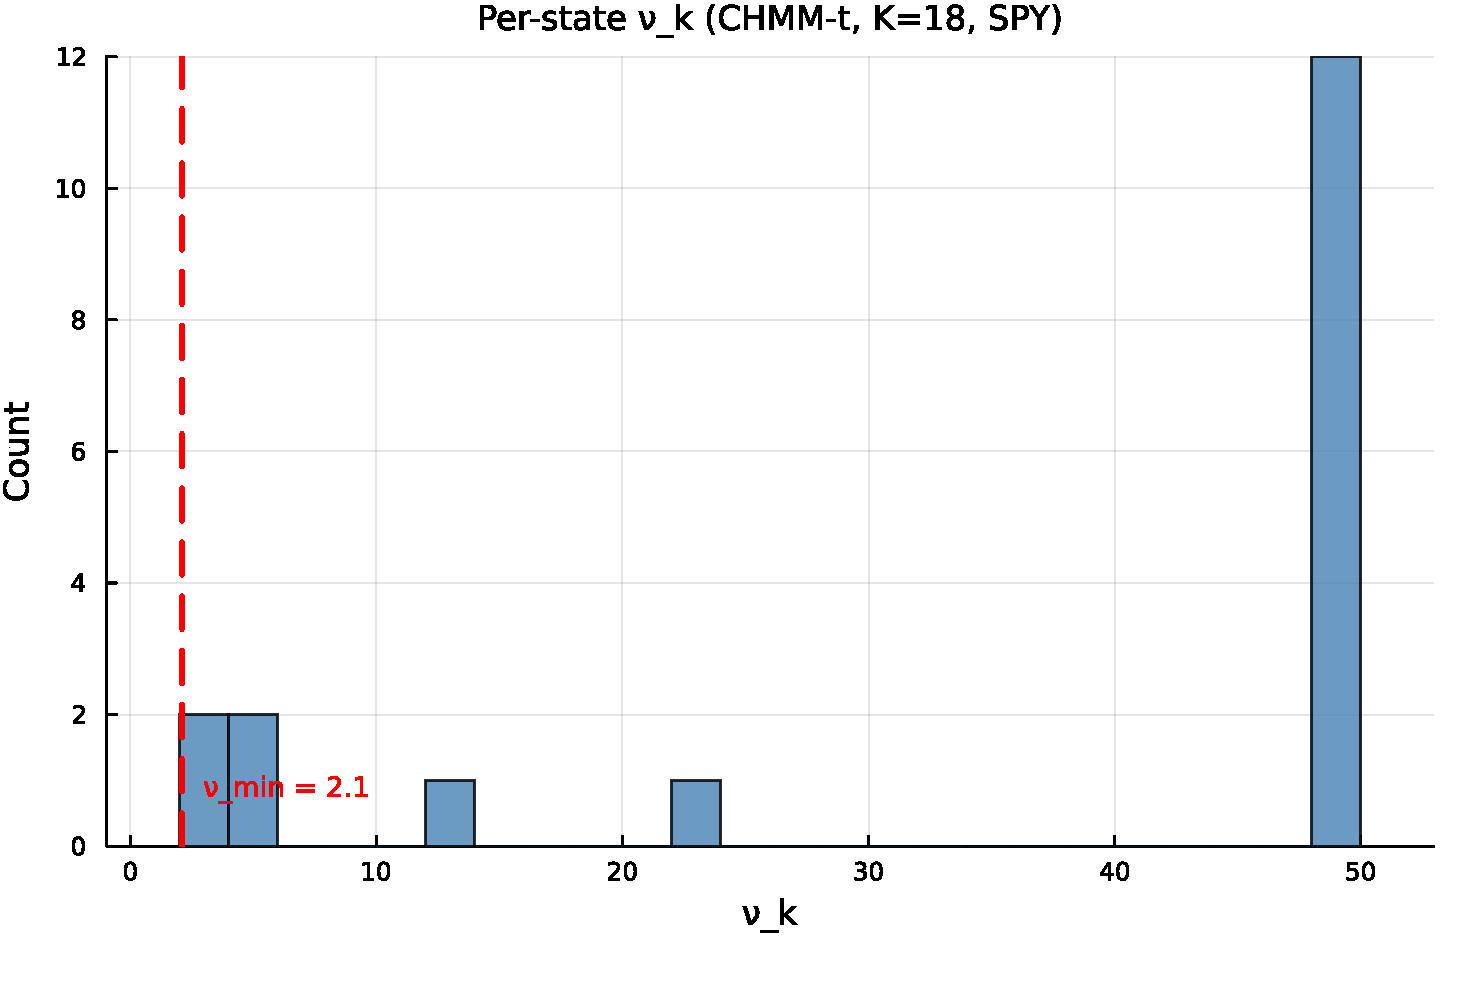
\includegraphics[width=0.65\textwidth]{figs/Fig-nu-Histogram.pdf}
\caption{Per-state degrees-of-freedom $\nu_k$ for the CHMM-t fit at $K = 18$ on SPY IS. The dashed red line marks the lower ECM bracket $\nu_{\min} = 2.1$. Only two states ($\nu_2 = 2.19$, $\nu_4 = 2.10$) sit near the lower bracket; the median $\nu_k$ is at the upper bracket.}
\label{fig:nu_hist}
\end{figure}

\paragraph{CHMM-GED per-state $p_k$ (Gaussian-bulk / Laplace-tail bimodality).}
The generator comparison reports and discusses the $\hat p_k$ partition (Figure~\ref{fig:p_hist}). Briefly, the $K = 18$ CHMM-GED fit on SPY IS was bimodal: eleven states attained exactly $p_k = 3.0$ (thirteen were Gaussian-like with $p_k \ge 1.85$), one state landed at intermediate $p_k = 1.6$, and four states clustered in the Laplace-shape regime $p_k \in [0.86, 1.24]$, concentrated in the high-volatility ranks. The smallest fitted $p_k$ on SPY was $0.86$, well clear of every $p_{\min}$ tested in the bracket sweep, so the lower bracket was non-binding. The bimodal partition replicated across $10$ Monte Carlo seeds and across the cross-asset universe (full robustness panel in the cross-asset robustness appendix).

\paragraph{Bracket-sensitivity sweeps.}
A CHMM-t bracket sweep on $\nu_{\min} \in \{2.1, 2.5, 3.0, 4.0, \infty\}$ at $K = 18$ showed that the excess kurtosis overshoot is a feature of the Student-$t$ emission at $K = 18$, not a lower-bracket artefact. The simulated IS excess kurtosis stayed in a heavy-tailed band across finite brackets and collapsed only in the full Gaussian limit. The analogous CHMM-GED sweep on $p_{\max} \in \{2.0, 2.5, 3.0, 3.5, 4.0\}$ left the non-Gaussian state count invariant, with Laplace-like states in $\{3,4,5\}$; tightening $p_{\max}$ from $4.0$ to $3.0$ cost only a few nats of LL. The $p_{\min}$ sweep on $\{0.5, 0.7, 0.85\}$ was fully degenerate: every floor produced an identical fit because the smallest observed $\hat p_k$ on SPY was $0.86$.


\paragraph{Evaluation summary.}
Observed growth rates $G_t$ are fit by Baum-Welch CHMM at the default $K^\star = 3$, with $K = 18$ retained as the sensitivity reference for excess kurtosis fidelity; $1{,}000$ paths are then simulated and per-asset metrics computed (Table~\ref{tab:model_comparison}). For the multi-asset analysis we reuse the per-asset $K^\star = 3$ fits as marginals, draw a copula sample $\mathbf U \sim \mathcal C(\Sigma)$ from the fitted Student-$t$ copula on ranks, rank-reorder the per-asset single-asset paths to match $\mathbf U$, and report cross-asset metrics (Table~\ref{tab:cross_asset}). The single-asset CHMM framework is shared across both; the CHMM training and simulation steps are Algorithms~\ref{alg:chmm_em} and~\ref{alg:chmm_simulate}, the cross-asset rank-reordering step is Algorithm~\ref{alg:copula_sim}, and the architecture diagram for the single-asset framework is Figure~\ref{fig:chmm_architecture}.


\subsection{Validation Metric Details}
\label{sec:supp_metrics}
\subsection{Validation Metric Details}
\label{sec:metric_details}

This appendix documents the precise form of the seven per-path metrics referenced in Section~\ref{sec:metrics}.
For each model, 1{,}000 independent paths of length $T$ are simulated (200 paths for the cross-asset extension) and each metric is computed per path before aggregation.

\paragraph{Kolmogorov--Smirnov (KS) pass rate.}
The two-sample KS statistic \cite{kolmogorov1933, smirnov1948} measures the maximum vertical distance between two empirical CDFs,
\begin{equation}
    D_{n,m} = \sup_x |F_n(x) - G_m(x)|.
    \label{eq:ks}
\end{equation}
The KS pass rate is the fraction of paths for which the test fails to reject distributional equivalence against the reference data at $\alpha = 0.05$.

\paragraph{Anderson--Darling (AD) pass rate.}
The AD test is the integrated squared CDF deviation with a quadratic tail weighting, making it more sensitive than KS to tail discrepancies.
The AD pass rate is the fraction of paths for which the two-sample AD test fails to reject at $\alpha = 0.05$.

\paragraph{Excess kurtosis.}
Mean simulated excess kurtosis across paths, compared to the observed value.
Given Gaussian emissions, the CHMM is expected to underestimate kurtosis relative to the heavy-tailed empirical distribution, and the shortfall is one of the reported diagnostics.

\paragraph{ACF-MAE.}
Mean absolute error between observed and mean-simulated autocorrelation functions of $|G_t|$ over $L = 252$ lags,
\begin{equation}
    \text{ACF-MAE} = \frac{1}{L}\sum_{\tau=1}^{L} \left| \hat\rho^{\text{obs}}_{|G|}(\tau) - \bar{\hat\rho}^{\,\text{sim}}_{|G|}(\tau) \right|.
    \label{eq:acf_mae_supp}
\end{equation}
This is the direct diagnostic for the Ryd\'{e}n et al.\ limitation.

\paragraph{Wasserstein-1 distance.}
The mean absolute difference of sorted empirical quantiles, equivalent to the $L^1$ distance between the empirical CDFs \cite{glasserman2003monte},
\begin{equation}
    W_1(F, G) = \int_0^1 |F^{-1}(u) - G^{-1}(u)|\, du.
    \label{eq:wasserstein}
\end{equation}

\paragraph{Hellinger distance.}
A histogram-based overlap distance in $[0, 1]$,
\begin{equation}
    H(P, Q) = \frac{1}{\sqrt{2}}\sqrt{\sum_{i=1}^{B}\left(\sqrt{p_i} - \sqrt{q_i}\right)^2},
    \label{eq:hellinger}
\end{equation}
with $B$ equal-width bins spanning the joint support and $p_i, q_i$ the observed and simulated bin probabilities.

\paragraph{Quantile coverage.}
The fraction of 99 equally-spaced observed quantiles (1st through 99th percentile) falling inside the 5th--95th percentile envelope of the corresponding simulated quantile across 1{,}000 paths.
A coverage of 100\% indicates that the simulation envelope fully brackets the observed distribution at every percentile.

\paragraph{Cross-asset metrics.}
For the cross-asset extension we additionally track the mean Frobenius norm $\|\hat\Sigma_{\text{sim}}^{(p)} - \hat\Sigma_{\text{obs}}\|_F$ and the off-diagonal Pearson correlation MAE between simulated and observed return matrices, averaged over paths.



\subsection{Formal Theoretical Statements}
\label{sec:supp_propositions}

The following propositions are referenced in Section~\ref{sec:theory} and stated formally here for reference; each is a one-line specialisation of a standard result and the proof sketch is one sentence.

\begin{proposition}[ECM monotonicity for CHMM-t (and EM monotonicity for CHMM-N, CHMM-L)]
\label{prop:ecm_monotone}
Under compactness of the parameter space ($\mu_k$, $\sigma_k$ or $b_k$, $\nu_k$ each in a closed bounded interval, $T_{ij} \ge \epsilon_T > 0$), the two-block CM step for CHMM-t of Section~\ref{sec:mstep}, namely the closed-form weighted updates of $(\mathbf T, \boldsymbol\pi, \mu_k, \sigma_k)$ at fixed $\nu_k$, followed by a golden-section maximisation of the per-state $Q$-function over $\nu_k \in [\nu_{\min}, \nu_{\max}]$, satisfies $Q(\theta^{(n+1)} \mid \theta^{(n)}) \ge Q(\theta^{(n)} \mid \theta^{(n)})$, and consequently $\mathcal L(\theta^{(n+1)}) \ge \mathcal L(\theta^{(n)})$ where $\mathcal L$ is the incomplete-data log-likelihood. The same monotonicity holds for the closed-form CHMM-N and CHMM-L M-steps under the standard EM guarantee.
\end{proposition}
\noindent\emph{Proof sketch.} Each CM step does not decrease $Q$ by definition (CM-1 is closed-form maximum, CM-2 is golden-section maximum); the standard EM inequality $\mathcal L(\theta^{(n+1)}) - \mathcal L(\theta^{(n)}) \ge Q(\theta^{(n+1)} \mid \theta^{(n)}) - Q(\theta^{(n)} \mid \theta^{(n)})$ \cite{wu1983convergence, mengrubin1993ecm} converts $Q$-monotonicity into log-likelihood monotonicity. Compactness gives boundedness above, hence convergence.

\begin{proposition}[Identifiability up to label permutation]
\label{prop:identifiability}
Under irreducibility and aperiodicity of $\mathbf T$ (Assumption~\ref{ass:irred}) and the emission contrast condition (Assumption~\ref{ass:moments}), the CHMM parameter is identifiable up to label permutation in all three emission families considered (CHMM-N, CHMM-t with $\nu_k \in [\nu_{\min}, \nu_{\max}]$, and CHMM-L).
\end{proposition}
\noindent\emph{Proof sketch.} The HMM identifiability theorem of \citet{allman2009identifiability} requires $\mathbf T$ of full rank and per-state emissions linearly independent in the space of densities on $\R$. Full-rank $\mathbf T$ follows from irreducibility \cite{levinperes2017markov}; linear independence of Gaussian, bracketed-$\nu$ Student-t, and Laplace emissions with distinct location-scale parameters follows from \citet{yakowitzspragins1968}.

\begin{proposition}[MLE consistency]
\label{prop:consistency}
Under Assumptions~\ref{ass:irred}--\ref{ass:moments} and the assumption that the true parameter lies in the interior of a compact $\Theta$, the MLE $\hat\theta_T = \arg\max_{\theta \in \Theta} \mathcal L_T(\theta)$ is consistent: $\hat\theta_T \xrightarrow{p} \theta_0$ as $T \to \infty$, modulo label permutation.
\end{proposition}
\noindent\emph{Proof reference.} \citet{bickel1998asymptotic} (Theorem~1) and \citet{doucmoulinesryden2004} apply directly under our assumption set: irreducibility supplies the mixing condition, finite second moment the moment condition, compactness the parameter-space condition.

\begin{proposition}[Marginal preservation under rank reordering]
\label{prop:rank_marginals}
Let $\tilde g_{j, 1:T}$ be a sample of size $T$ from the per-asset CHMM marginal of asset $j$, and let the rank-reordered output be $\hat g_{j,t}^{(p)} = \tilde g_{j, (r_{j,t}^{(p)})}^{(p)}$ where $r_{j,t}^{(p)}$ is the rank of the copula sample. Then for every asset $j$ the empirical CDF of $\{\hat g_{j,t}^{(p)}\}_{t=1}^T$ equals that of $\{\tilde g_{j,t}^{(p)}\}_{t=1}^T$.
\end{proposition}
\noindent\emph{Proof sketch.} The map $t \mapsto r_{j,t}^{(p)}$ is a permutation almost surely, so the multiset of values is preserved; the empirical CDF depends only on the multiset.

\subsection{State-Resolution and Multi-Emission Sensitivity}
\label{sec:supp_sensitivity}
\subsubsection{Full State-Resolution Sensitivity Table}
\label{sec:sensitivity_table}

Table~\ref{tab:sensitivity} reports the full $K$-sweep referenced in Section~\ref{sec:k_selection_results} of the main text.
Observed excess kurtosis is $7.68$ IS and $5.29$ OoS at all $K$.

\begin{table}[H]
\centering
\caption{State resolution sensitivity for SPY CHMM-N (1{,}000 paths, $\alpha = 0.05$). Every metric is computed on the identical simulation pipeline used for Table~\ref{tab:model_comparison} in the main text. IS coverage was 100\% at every $K$; OoS coverage is reported separately. ACF-MAE columns: $|G_t|$ measures the volatility-clustering reproduction; $G_t$ measures linear-autocorrelation reproduction (parallel to $|G_t|$, both averaged over lags 1--252).}
\label{tab:sensitivity}
\small
\begin{tabular}{c cc cc cc cc c c c}
\toprule
& \multicolumn{2}{c}{KS (\%)} & \multicolumn{2}{c}{AD (\%)} & \multicolumn{2}{c}{Kurtosis} & \multicolumn{2}{c}{ACF-MAE} & & & \\
\cmidrule(lr){2-3} \cmidrule(lr){4-5} \cmidrule(lr){6-7} \cmidrule(lr){8-9}
$K$ & IS & OoS & IS & OoS & Obs & Sim & $|G_t|$ & $G_t$ & $W_1$ & $H$ & Cov OoS (\%) \\
\midrule
3  & 89.0 & 77.2 & 78.9 & 68.6 & 7.68 & 3.82 & 0.0463 & 0.0240 & 0.131 & 0.0839 & 94.9 \\
6  & 92.9 & 78.7 & 84.3 & 74.3 & 7.68 & 5.38 & 0.0496 & 0.0238 & 0.116 & 0.0829 & 90.9 \\
9  & 93.0 & 81.4 & 84.4 & 74.4 & 7.68 & 4.63 & 0.0492 & 0.0238 & 0.118 & 0.0810 & 91.9 \\
12 & 94.9 & 81.6 & 85.8 & 75.0 & 7.68 & 4.57 & 0.0500 & 0.0238 & 0.113 & 0.0801 & 91.9 \\
15 & 93.9 & 81.0 & 84.8 & 73.5 & 7.68 & 4.89 & 0.0508 & 0.0238 & 0.114 & 0.0804 & 88.9 \\
\textbf{18} & 94.8 & 85.5 & 88.2 & 79.7 & 7.68 & 5.04 & 0.0515 & 0.0237 & 0.110 & 0.0807 & 91.9 \\
21 & \textbf{95.6} & \textbf{88.0} & \textbf{89.1} & \textbf{78.8} & 7.68 & 3.78 & 0.0534 & \textbf{0.0236} & 0.112 & 0.0801 & \textbf{99.0} \\
\bottomrule
\end{tabular}
\end{table}

\subsubsection{Multi-Emission State-Resolution Sensitivity}
\label{sec:multi_emission_sensitivity}

Table~\ref{tab:sensitivity_multi} extends Table~\ref{tab:sensitivity} across the three emission families, confirming that the qualitative operating point $K = 18$ is stable when the Gaussian component is replaced with Student-t or Laplace emissions.
For CHMM-t the per-state degrees of freedom $\nu_k$ are refit by ECM-plus-golden-section at every $K$; for CHMM-L the weighted-median location and weighted MAD scale are closed form and impose no additional cost.
Three patterns extend from Table~\ref{tab:sensitivity} to the new families.
First, the distributional pass rates plateau in the $K \in \{12, 15, 18, 21\}$ band for all three families: CHMM-t reaches its highest IS KS at $K = 18$ ($96.0\%$) and its highest OoS KS at $K = 18$ ($84.5\%$), and CHMM-L reaches its highest IS KS at $K = 18$ ($95.6\%$) and its highest IS AD at $K = 18$ ($92.7\%$).
Once a family enters the plateau the operating point is flat with respect to $K$, so we report the main-text results at the same $K = 18$ used for CHMM-N.
Second, the absolute-return ACF-MAE remains within the narrow $0.047$--$0.056$ band observed for the Gaussian sweep, and the raw-return ACF-MAE remains essentially constant at $\approx 0.024$ across all $21$ (family, $K$) combinations. Both temporal axes are properties of the regime structure rather than the emission family: $|G_t|$ ACF reproduction is governed by the eigenvalue spectrum of $\mathbf T$ (Section~\ref{sec:theory}), and raw-$G_t$ ACF is null in expectation under any HMM with i.i.d.\ within-state emissions.
Third, simulated kurtosis behaves as expected from the component families: the Gaussian sweep peaks around $5.0$ at the high-$K$ end, the Laplace sweep lands squarely in the $5.3$--$6.7$ range (closest to the observed $7.68$), and the Student-t sweep climbs sharply above $13$ across the entire sweep because the ECM search assigns small $\nu_k$ to a subset of tail states, over-correcting IS kurtosis.

\begin{table}[H]
\centering
\caption{Multi-emission state resolution sensitivity for SPY (1{,}000 paths, $\alpha = 0.05$). CHMM-N: Gaussian; CHMM-t: Student-t with per-state $\nu_k$ refit by ECM-plus-golden-section; CHMM-L: Laplace with weighted-median location and weighted-MAD scale. Every metric is computed on the identical simulation pipeline used for Table~\ref{tab:model_comparison}. Observed excess kurtosis is $7.68$ IS and $5.29$ OoS. ACF-MAE columns parallel the main-text Table~\ref{tab:model_comparison}: $|G_t|$ for volatility clustering, $G_t$ (raw) for linear autocorrelation.}
\label{tab:sensitivity_multi}
\small
\resizebox{\textwidth}{!}{%
\begin{tabular}{l c cc cc c cc c c}
\toprule
& & \multicolumn{2}{c}{KS (\%)} & \multicolumn{2}{c}{AD (\%)} & & \multicolumn{2}{c}{ACF-MAE} & & \\
\cmidrule(lr){3-4} \cmidrule(lr){5-6} \cmidrule(lr){8-9}
Family & $K$ & IS & OoS & IS & OoS & Kurt (IS sim) & $|G_t|$ & $G_t$ & $W_1$ IS & $H$ IS \\
\midrule
CHMM-N & 3  & 89.7 & 80.1 & 79.2 & 70.7 & 3.86  & 0.0467 & 0.0240 & 0.128 & 0.0833 \\
       & 6  & 93.8 & 79.1 & 87.2 & 72.8 & 5.29  & 0.0504 & 0.0238 & 0.114 & 0.0825 \\
       & 9  & 94.9 & 83.0 & 84.3 & 74.8 & 4.58  & 0.0490 & 0.0238 & 0.115 & 0.0806 \\
       & 12 & 93.7 & 82.7 & 85.5 & 75.0 & 4.56  & 0.0501 & 0.0237 & 0.115 & 0.0804 \\
       & 15 & 93.6 & 83.0 & 87.0 & 75.1 & 4.89  & 0.0509 & 0.0238 & 0.114 & 0.0803 \\
       & \textbf{18} & 94.7 & 83.4 & 88.5 & 76.6 & 4.97  & 0.0511 & 0.0237 & 0.108 & 0.0805 \\
       & 21 & \textbf{95.1} & \textbf{88.0} & \textbf{88.2} & \textbf{79.7} & 3.80  & 0.0532 & 0.0236 & 0.110 & 0.0796 \\
\midrule
CHMM-t & 3  & 92.2 & 82.9 & 88.0 & 79.1 & 33.68 & 0.0538 & 0.0235 & 0.108 & 0.0759 \\
       & 6  & 91.8 & 80.4 & 86.7 & 74.8 & 22.74 & 0.0527 & 0.0235 & 0.108 & 0.0772 \\
       & 9  & 95.4 & 84.0 & 89.9 & 78.0 & 16.60 & 0.0535 & 0.0234 & 0.102 & 0.0752 \\
       & 12 & 95.2 & 85.0 & 89.8 & 78.4 & 14.98 & 0.0543 & 0.0234 & 0.100 & 0.0757 \\
       & 15 & 94.7 & 83.7 & 88.8 & 79.5 & 16.36 & 0.0539 & 0.0234 & 0.101 & 0.0758 \\
       & \textbf{18} & \textbf{96.0} & \textbf{84.5} & \textbf{91.7} & \textbf{80.8} & 13.19 & 0.0551 & \textbf{0.0234} & \textbf{0.099} & \textbf{0.0759} \\
       & 21 & 94.5 & 83.3 & 88.5 & 78.1 & 14.66 & 0.0539 & 0.0234 & 0.102 & 0.0758 \\
\midrule
CHMM-L & 3  & 81.9 & 64.8 & 82.5 & 65.8 & 5.29  & 0.0535 & 0.0235 & 0.112 & 0.0854 \\
       & 6  & 90.5 & 76.4 & 85.0 & 74.2 & 5.91  & 0.0513 & 0.0235 & 0.110 & 0.0818 \\
       & 9  & 90.5 & 75.7 & 84.8 & 70.1 & 6.01  & 0.0517 & 0.0235 & 0.110 & 0.0819 \\
       & 12 & 93.6 & 81.4 & 89.8 & 78.8 & 6.18  & 0.0541 & 0.0234 & 0.106 & 0.0796 \\
       & 15 & 92.5 & 78.9 & 88.3 & 78.8 & 6.03  & 0.0541 & 0.0234 & 0.105 & 0.0792 \\
       & \textbf{18} & \textbf{95.6} & \textbf{79.9} & \textbf{92.7} & \textbf{80.7} & \textbf{6.74}  & 0.0563 & 0.0234 & 0.101 & 0.0798 \\
       & 21 & 93.1 & 79.5 & 87.7 & 76.8 & 6.05  & 0.0543 & 0.0234 & 0.107 & 0.0807 \\
\bottomrule
\end{tabular}%
}
\end{table}

\subsubsection{Baum-Welch Convergence}
\label{sec:convergence}

Figure~\ref{fig:convergence_all} shows the Baum-Welch convergence curves for representative state resolutions.
All models converged within the 60-iteration budget, with the log-likelihood monotonically increasing (as guaranteed by the EM algorithm).
Lower $K$ values typically converged faster (15--25 iterations), while higher $K$ values required 25--40 iterations to reach the convergence tolerance of $|\Delta\mathcal{L}| < 10^{-4}$.
The monotonic increase confirms that the quantile-based initialization provided a valid starting point from which the EM algorithm could improve without encountering degenerate solutions.

\begin{figure}[H]
\centering
\begin{subfigure}[b]{0.32\textwidth}
    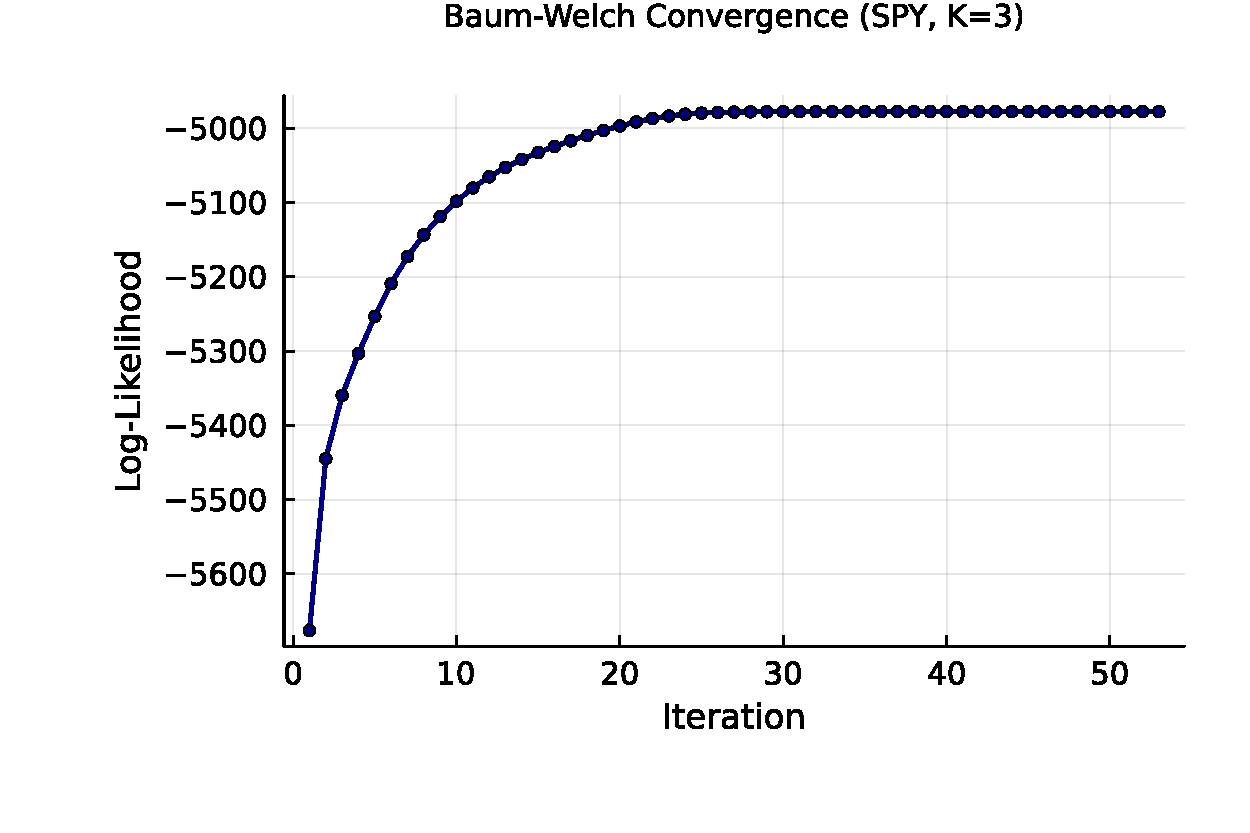
\includegraphics[width=\textwidth]{figs/Fig-Convergence-K3.pdf}
    \caption{$K = 3$}
\end{subfigure}
\hfill
\begin{subfigure}[b]{0.32\textwidth}
    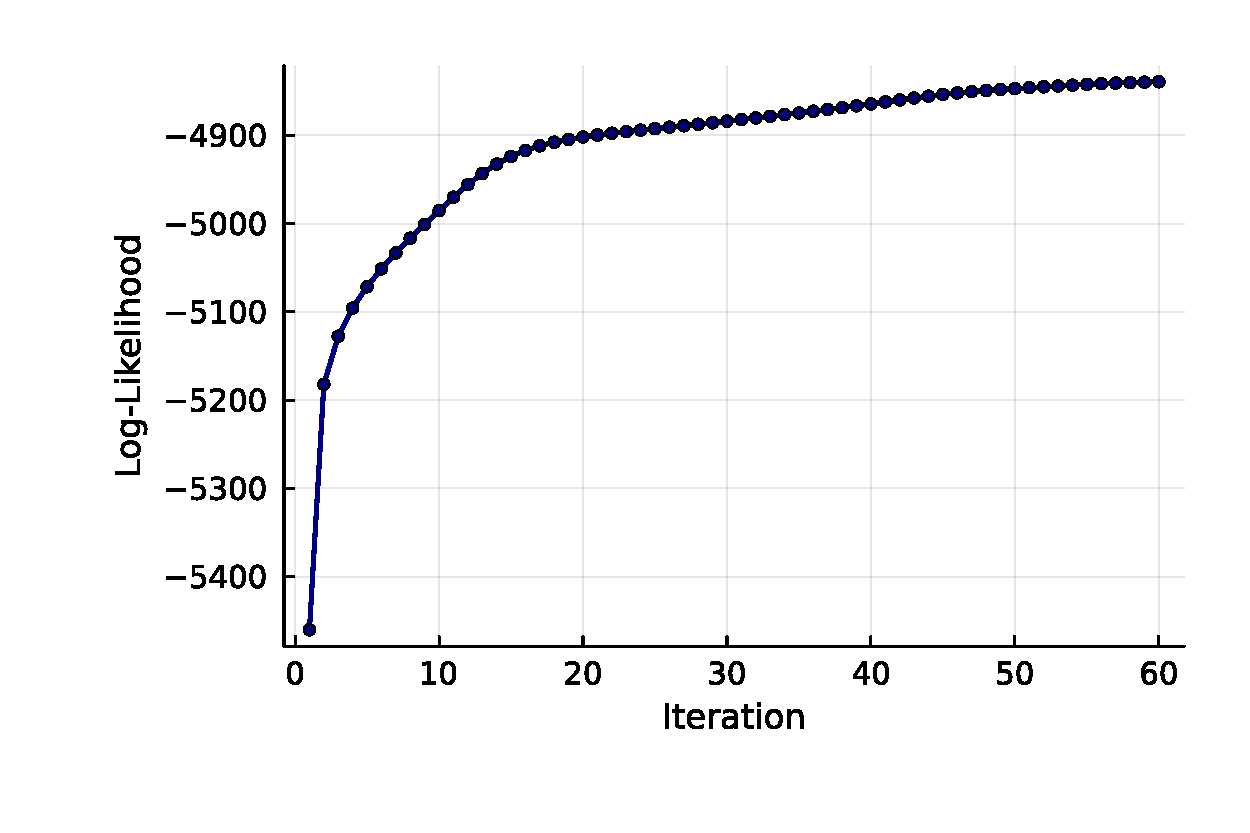
\includegraphics[width=\textwidth]{figs/Fig-Convergence-K12.pdf}
    \caption{$K = 12$}
\end{subfigure}
\hfill
\begin{subfigure}[b]{0.32\textwidth}
    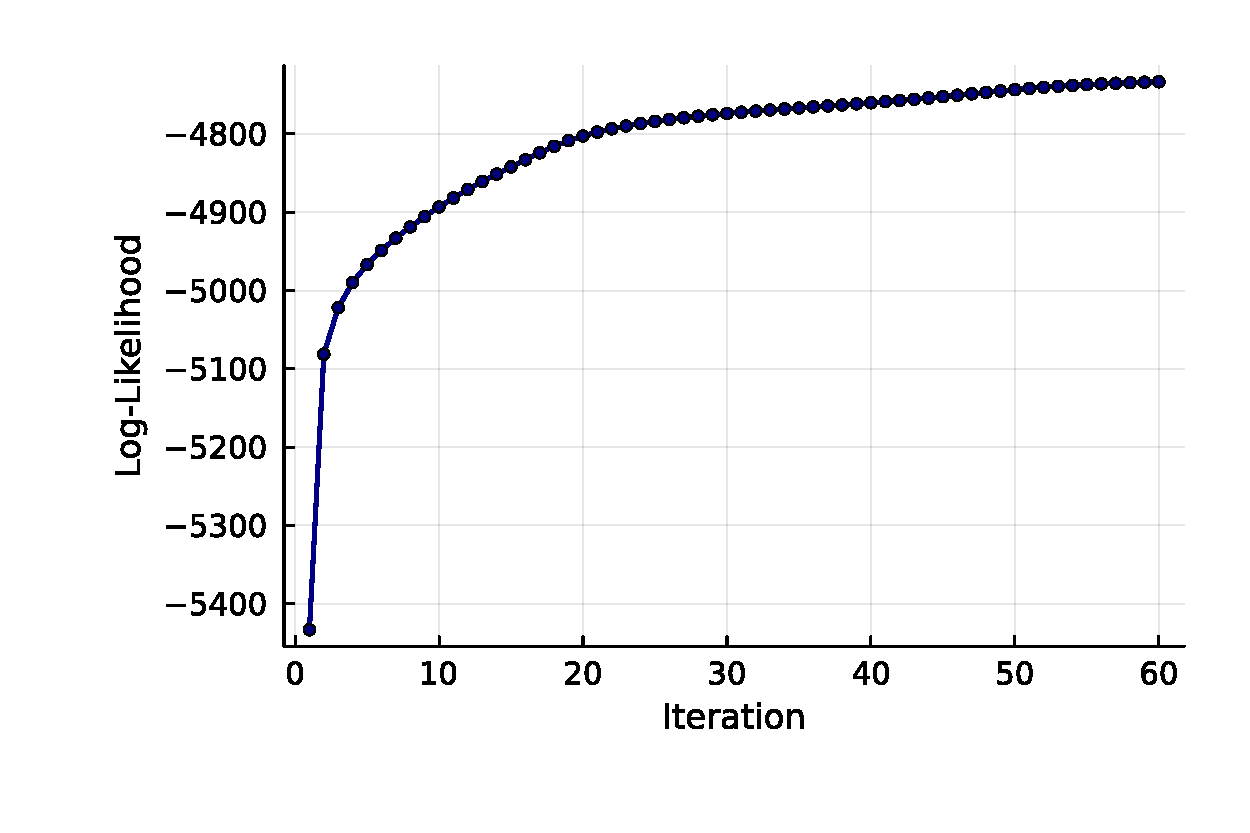
\includegraphics[width=\textwidth]{figs/Fig-Convergence-K18.pdf}
    \caption{$K = 18$ (selected)}
\end{subfigure}
\caption{Baum-Welch convergence for the SPY CHMM-N fit (Pipeline~A, IS) at selected state resolutions. Log-likelihood is monotonically increasing (EM guarantee) and plateaus well before $\texttt{max\_iter} = 60$.}
\label{fig:convergence_all}
\end{figure}

\subsubsection{IS Comparison at Non-Selected State Resolutions}
\label{sec:k_sweep_panels}

Figures~\ref{fig:k_sweep_panels_is}--\ref{fig:k_sweep_is_k21} show the IS model comparison panels for $K \in \{3, 6, 12, 21\}$, complementing the $K = 18$ comparison in Figure~\ref{fig:is_comparison} of the main text.
Across all resolutions, the CHMM's simulated density closely overlays the observed density, and the ACF of absolute returns tracks the slow decay pattern.
The visible improvement from $K = 3$ to $K = 18$ is concentrated in the tails of the Q-Q panel and the steady-state level of the ACF panel.
$K = 9$ and $K = 15$ panels are omitted because they interpolate smoothly between the shown resolutions; their numerical metrics are in Table~\ref{tab:sensitivity}.

\begin{figure}[H]
\centering
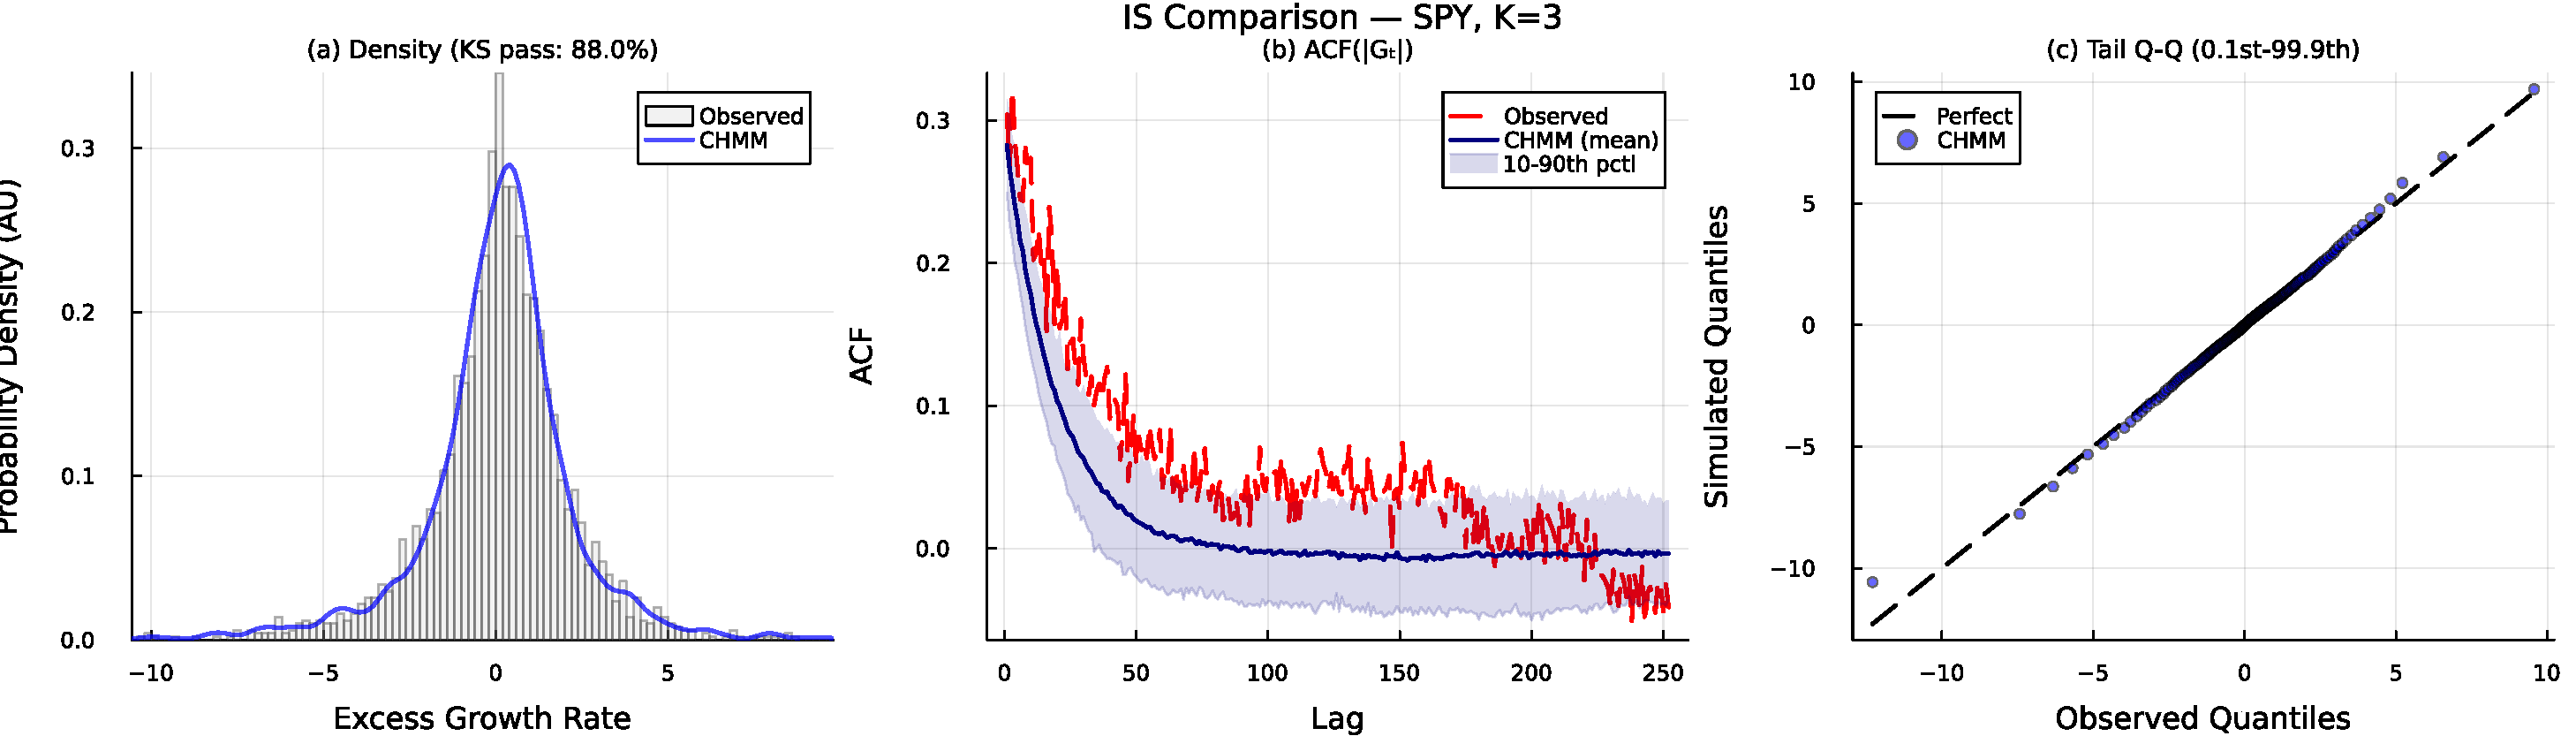
\includegraphics[width=\textwidth]{figs/Fig-3-IS-Comparison-K3.pdf}
\caption{IS SPY CHMM-N comparison at $K = 3$ (Pipeline~A, 1{,}000 simulated paths; panels as in Figure~\ref{fig:is_comparison}). The $K = 18$ counterpart is Figure~\ref{fig:is_comparison} of the main text.}
\label{fig:k_sweep_panels_is}
\end{figure}

\begin{figure}[H]
\centering
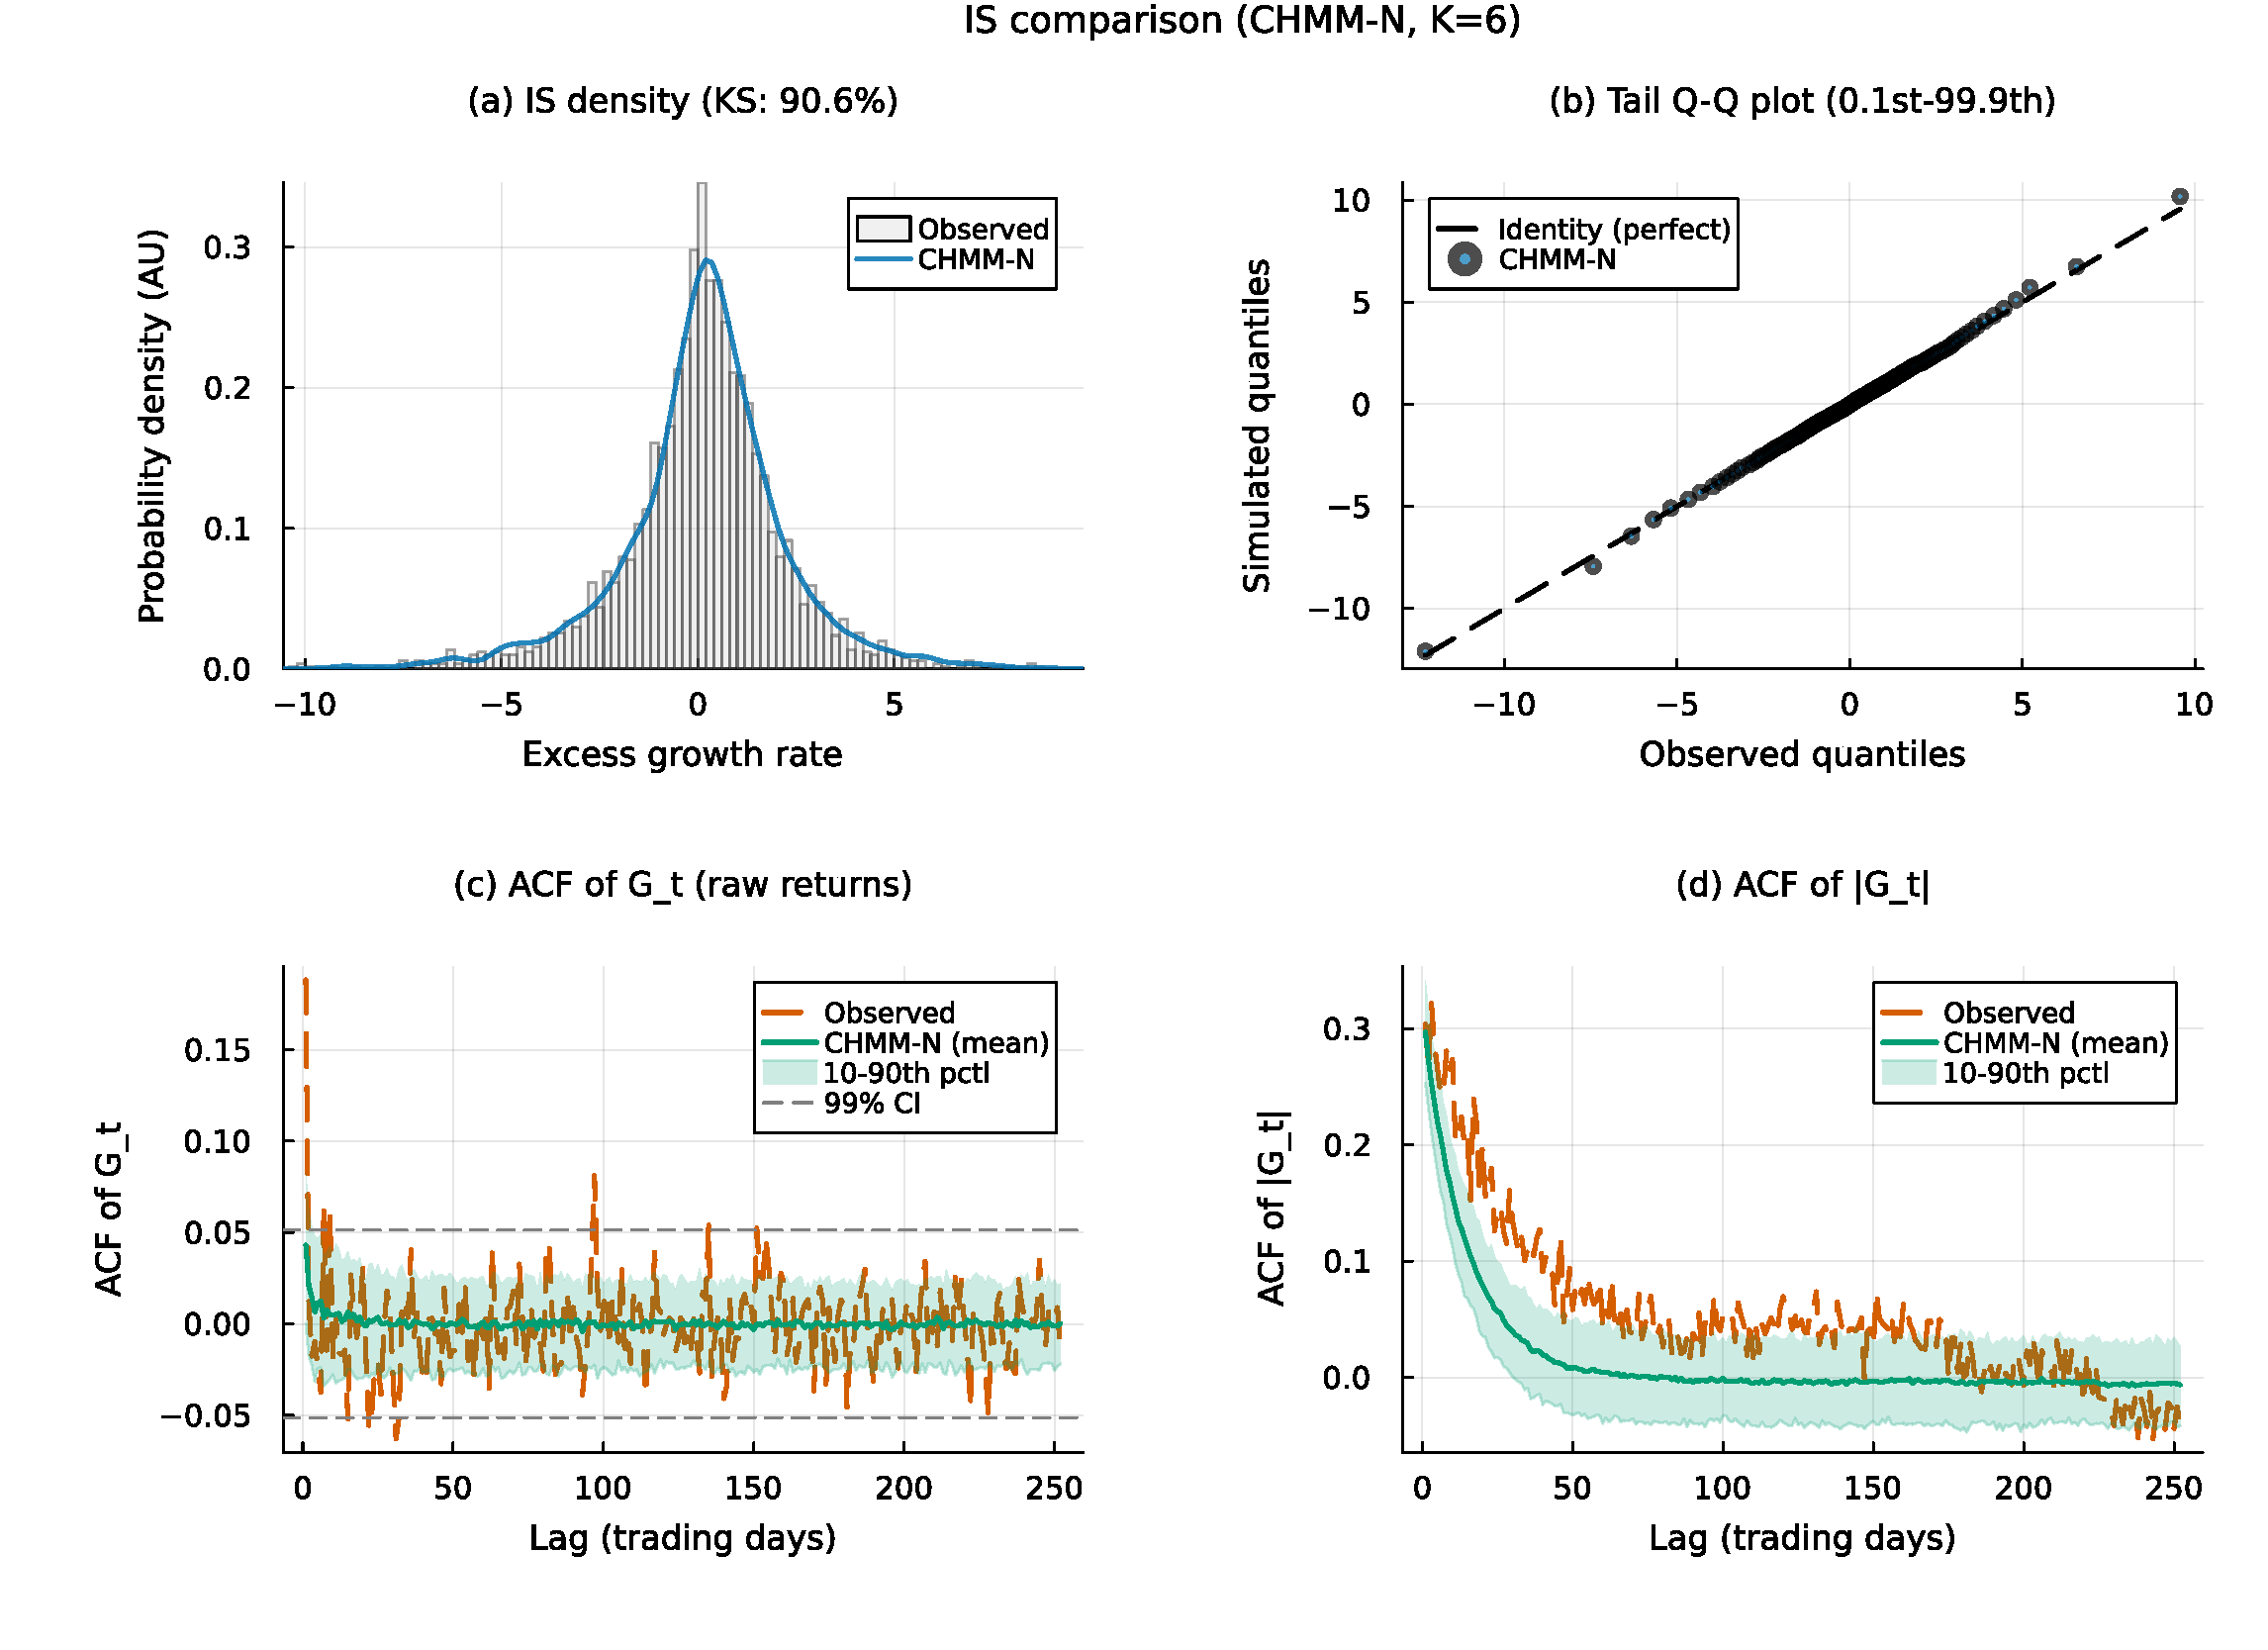
\includegraphics[width=\textwidth]{figs/Fig-3-IS-Comparison-K6.pdf}
\caption{IS SPY CHMM-N comparison at $K = 6$ (Pipeline~A, 1{,}000 simulated paths; panels as in Figure~\ref{fig:is_comparison}).}
\label{fig:k_sweep_is_k6}
\end{figure}

\begin{figure}[H]
\centering
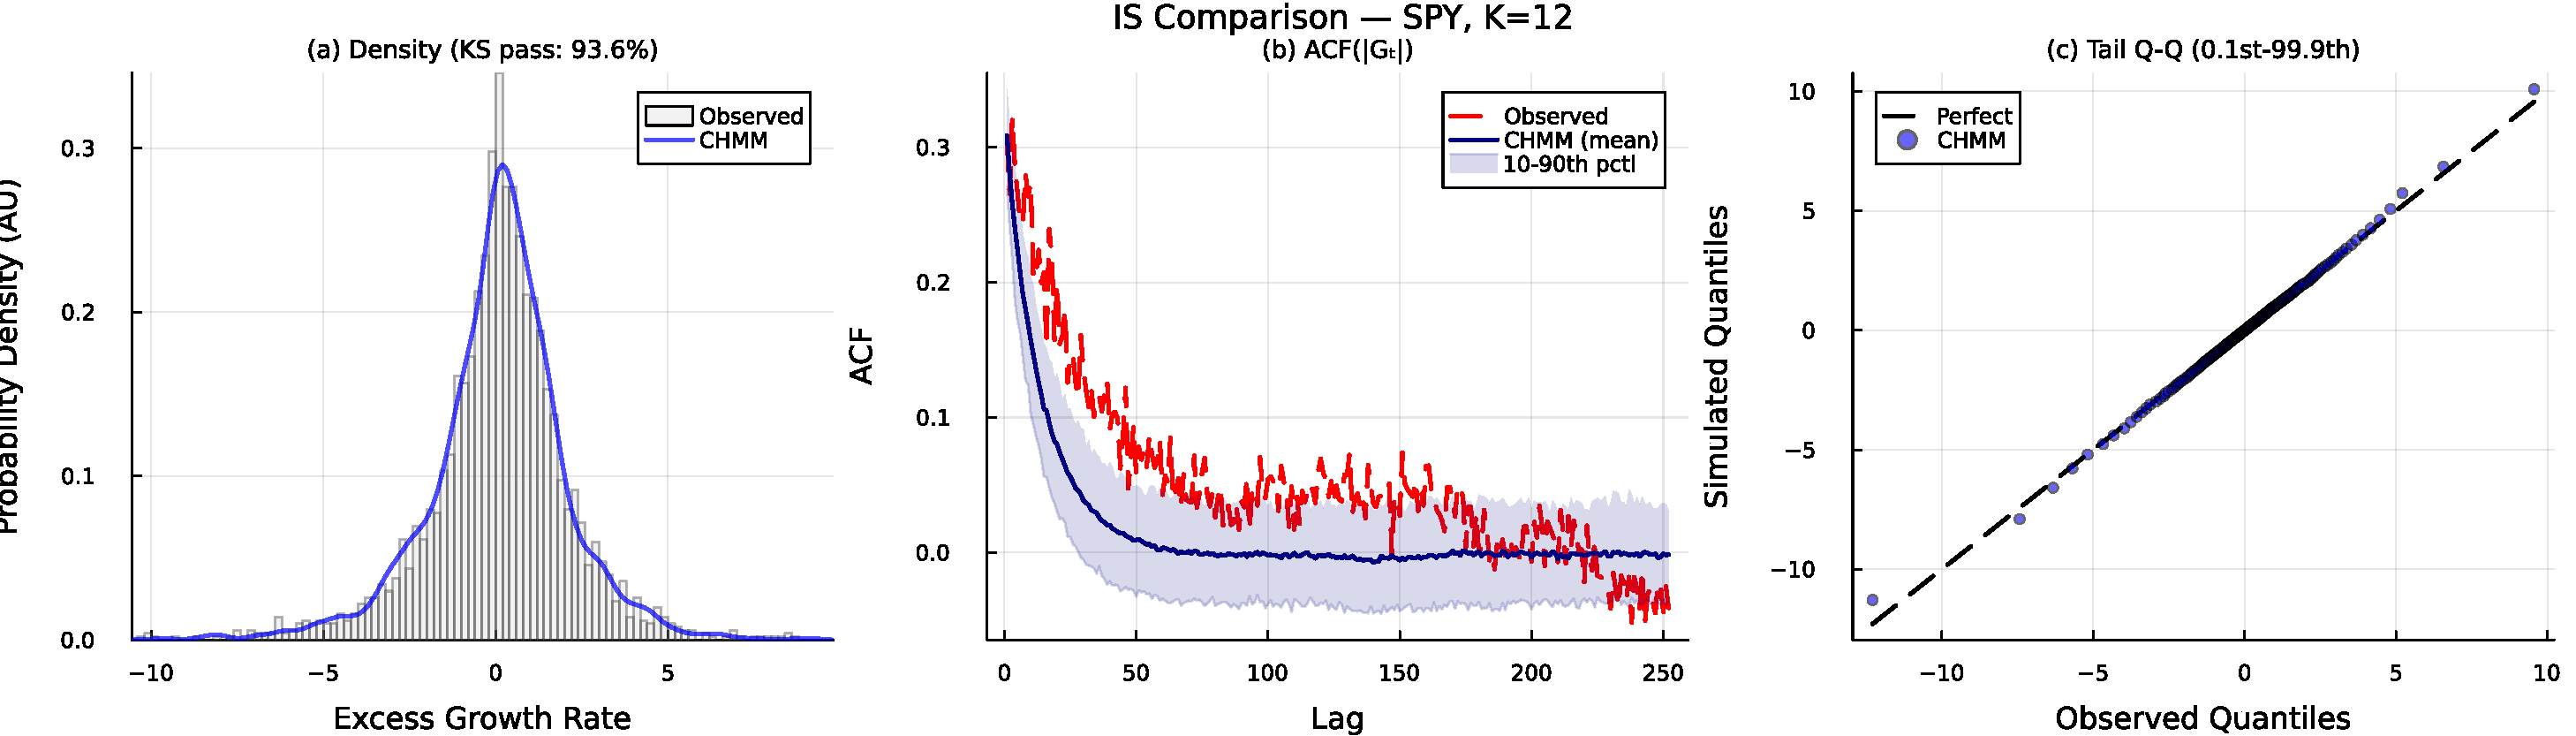
\includegraphics[width=\textwidth]{figs/Fig-3-IS-Comparison-K12.pdf}
\caption{IS SPY CHMM-N comparison at $K = 12$ (Pipeline~A, 1{,}000 simulated paths; panels as in Figure~\ref{fig:is_comparison}).}
\label{fig:k_sweep_is_k12}
\end{figure}

\begin{figure}[H]
\centering
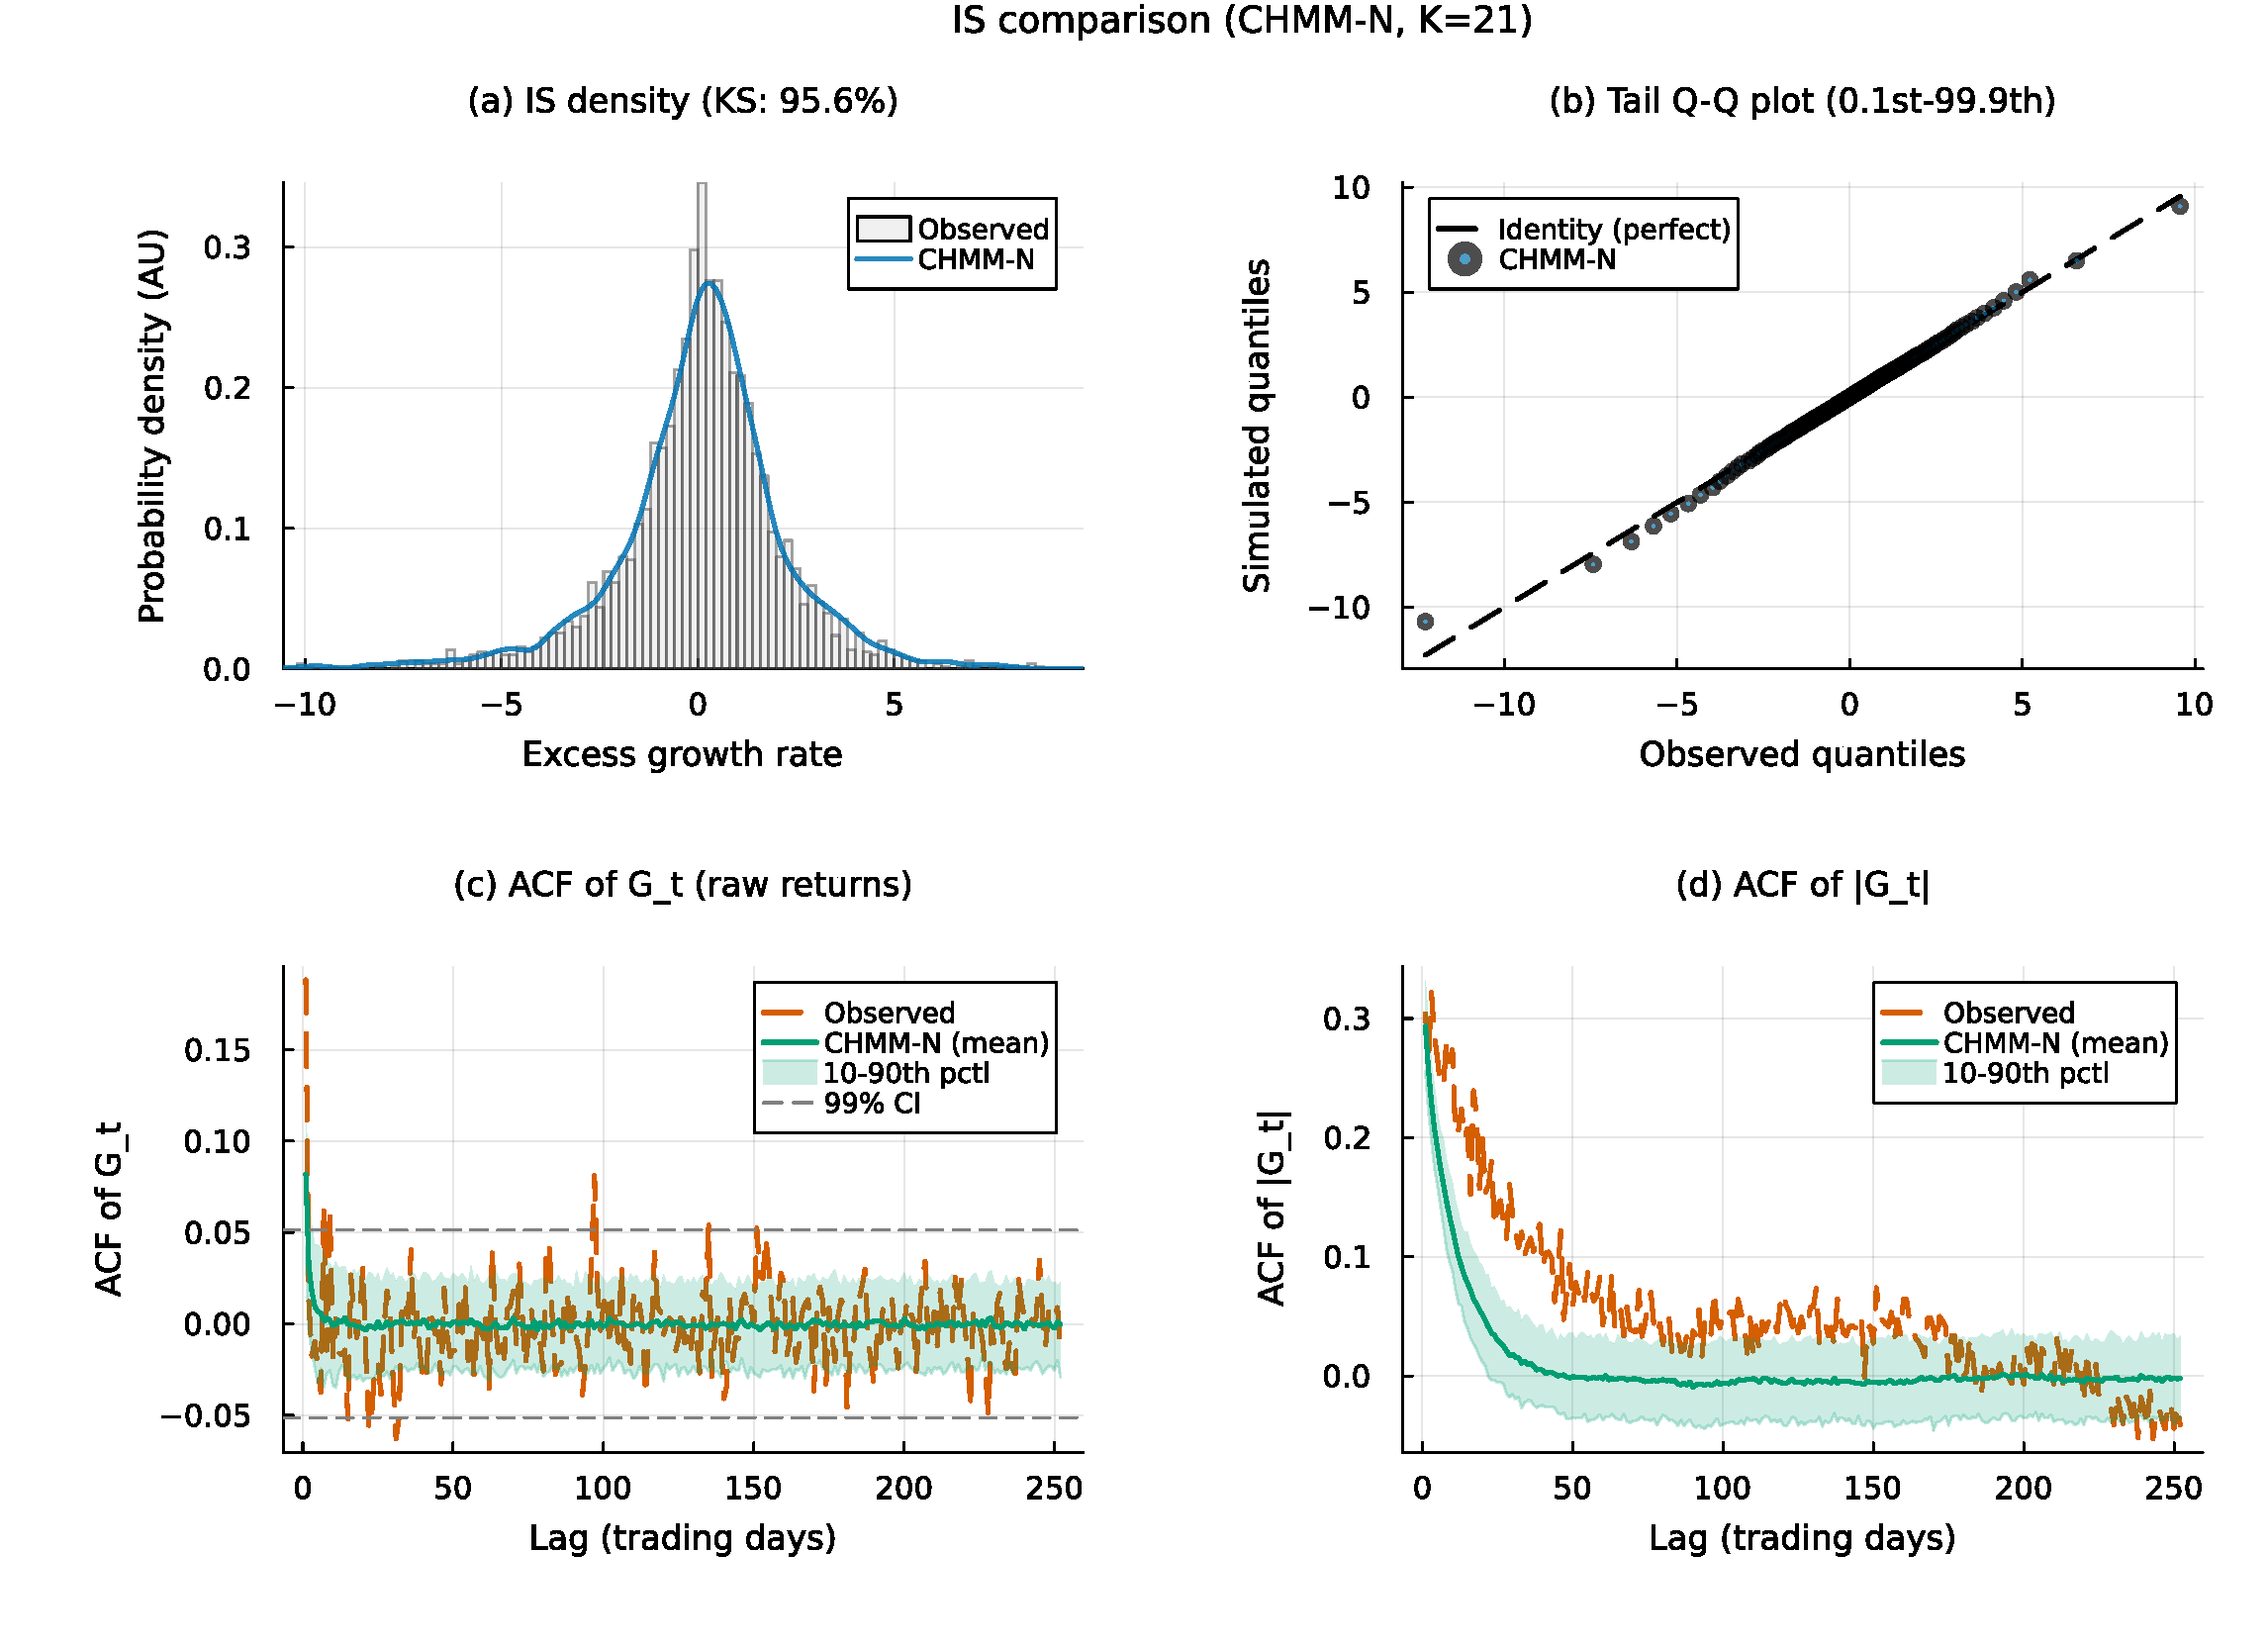
\includegraphics[width=\textwidth]{figs/Fig-3-IS-Comparison-K21.pdf}
\caption{IS SPY CHMM-N comparison at $K = 21$ (Pipeline~A, 1{,}000 simulated paths; panels as in Figure~\ref{fig:is_comparison}).}
\label{fig:k_sweep_is_k21}
\end{figure}

\subsubsection{OoS Validation at Non-Selected State Resolutions}

Figures~\ref{fig:k_sweep_panels_oos}--\ref{fig:k_sweep_oos_k21} show the OoS validation panels for $K \in \{3, 6, 12, 21\}$.
KS pass rates remain above 91\% at all resolutions; the $K = 18$ panel is reproduced in Figure~\ref{fig:oos_validation} of the main text.
As with the IS panels, $K = 9$ and $K = 15$ are omitted; numerical OoS KS pass rates are in Table~\ref{tab:sensitivity}.

\begin{figure}[H]
\centering
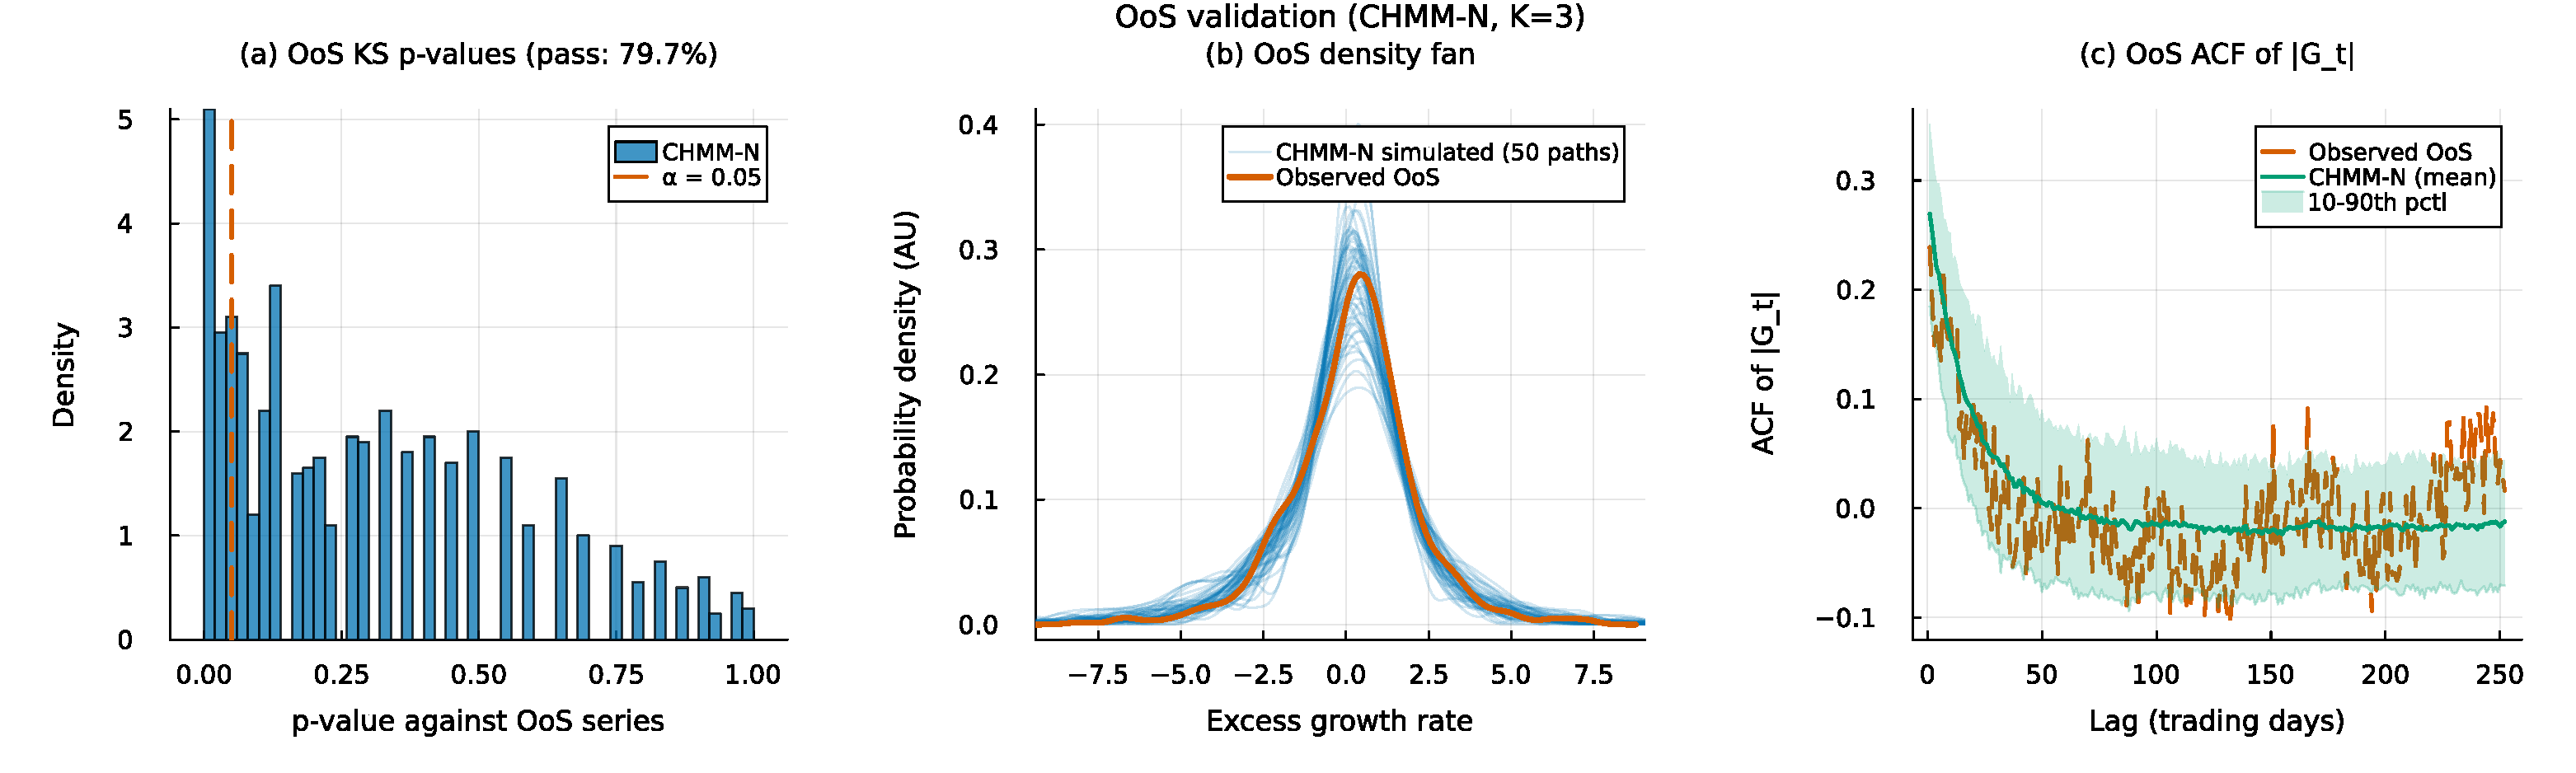
\includegraphics[width=\textwidth]{figs/Fig-4-OoS-Validation-K3.pdf}
\caption{OoS SPY CHMM-N validation at $K = 3$ (Pipeline~A, 1{,}000 simulated paths; panels as in Figure~\ref{fig:oos_validation}). The $K = 18$ counterpart is Figure~\ref{fig:oos_validation} of the main text.}
\label{fig:k_sweep_panels_oos}
\end{figure}

\begin{figure}[H]
\centering
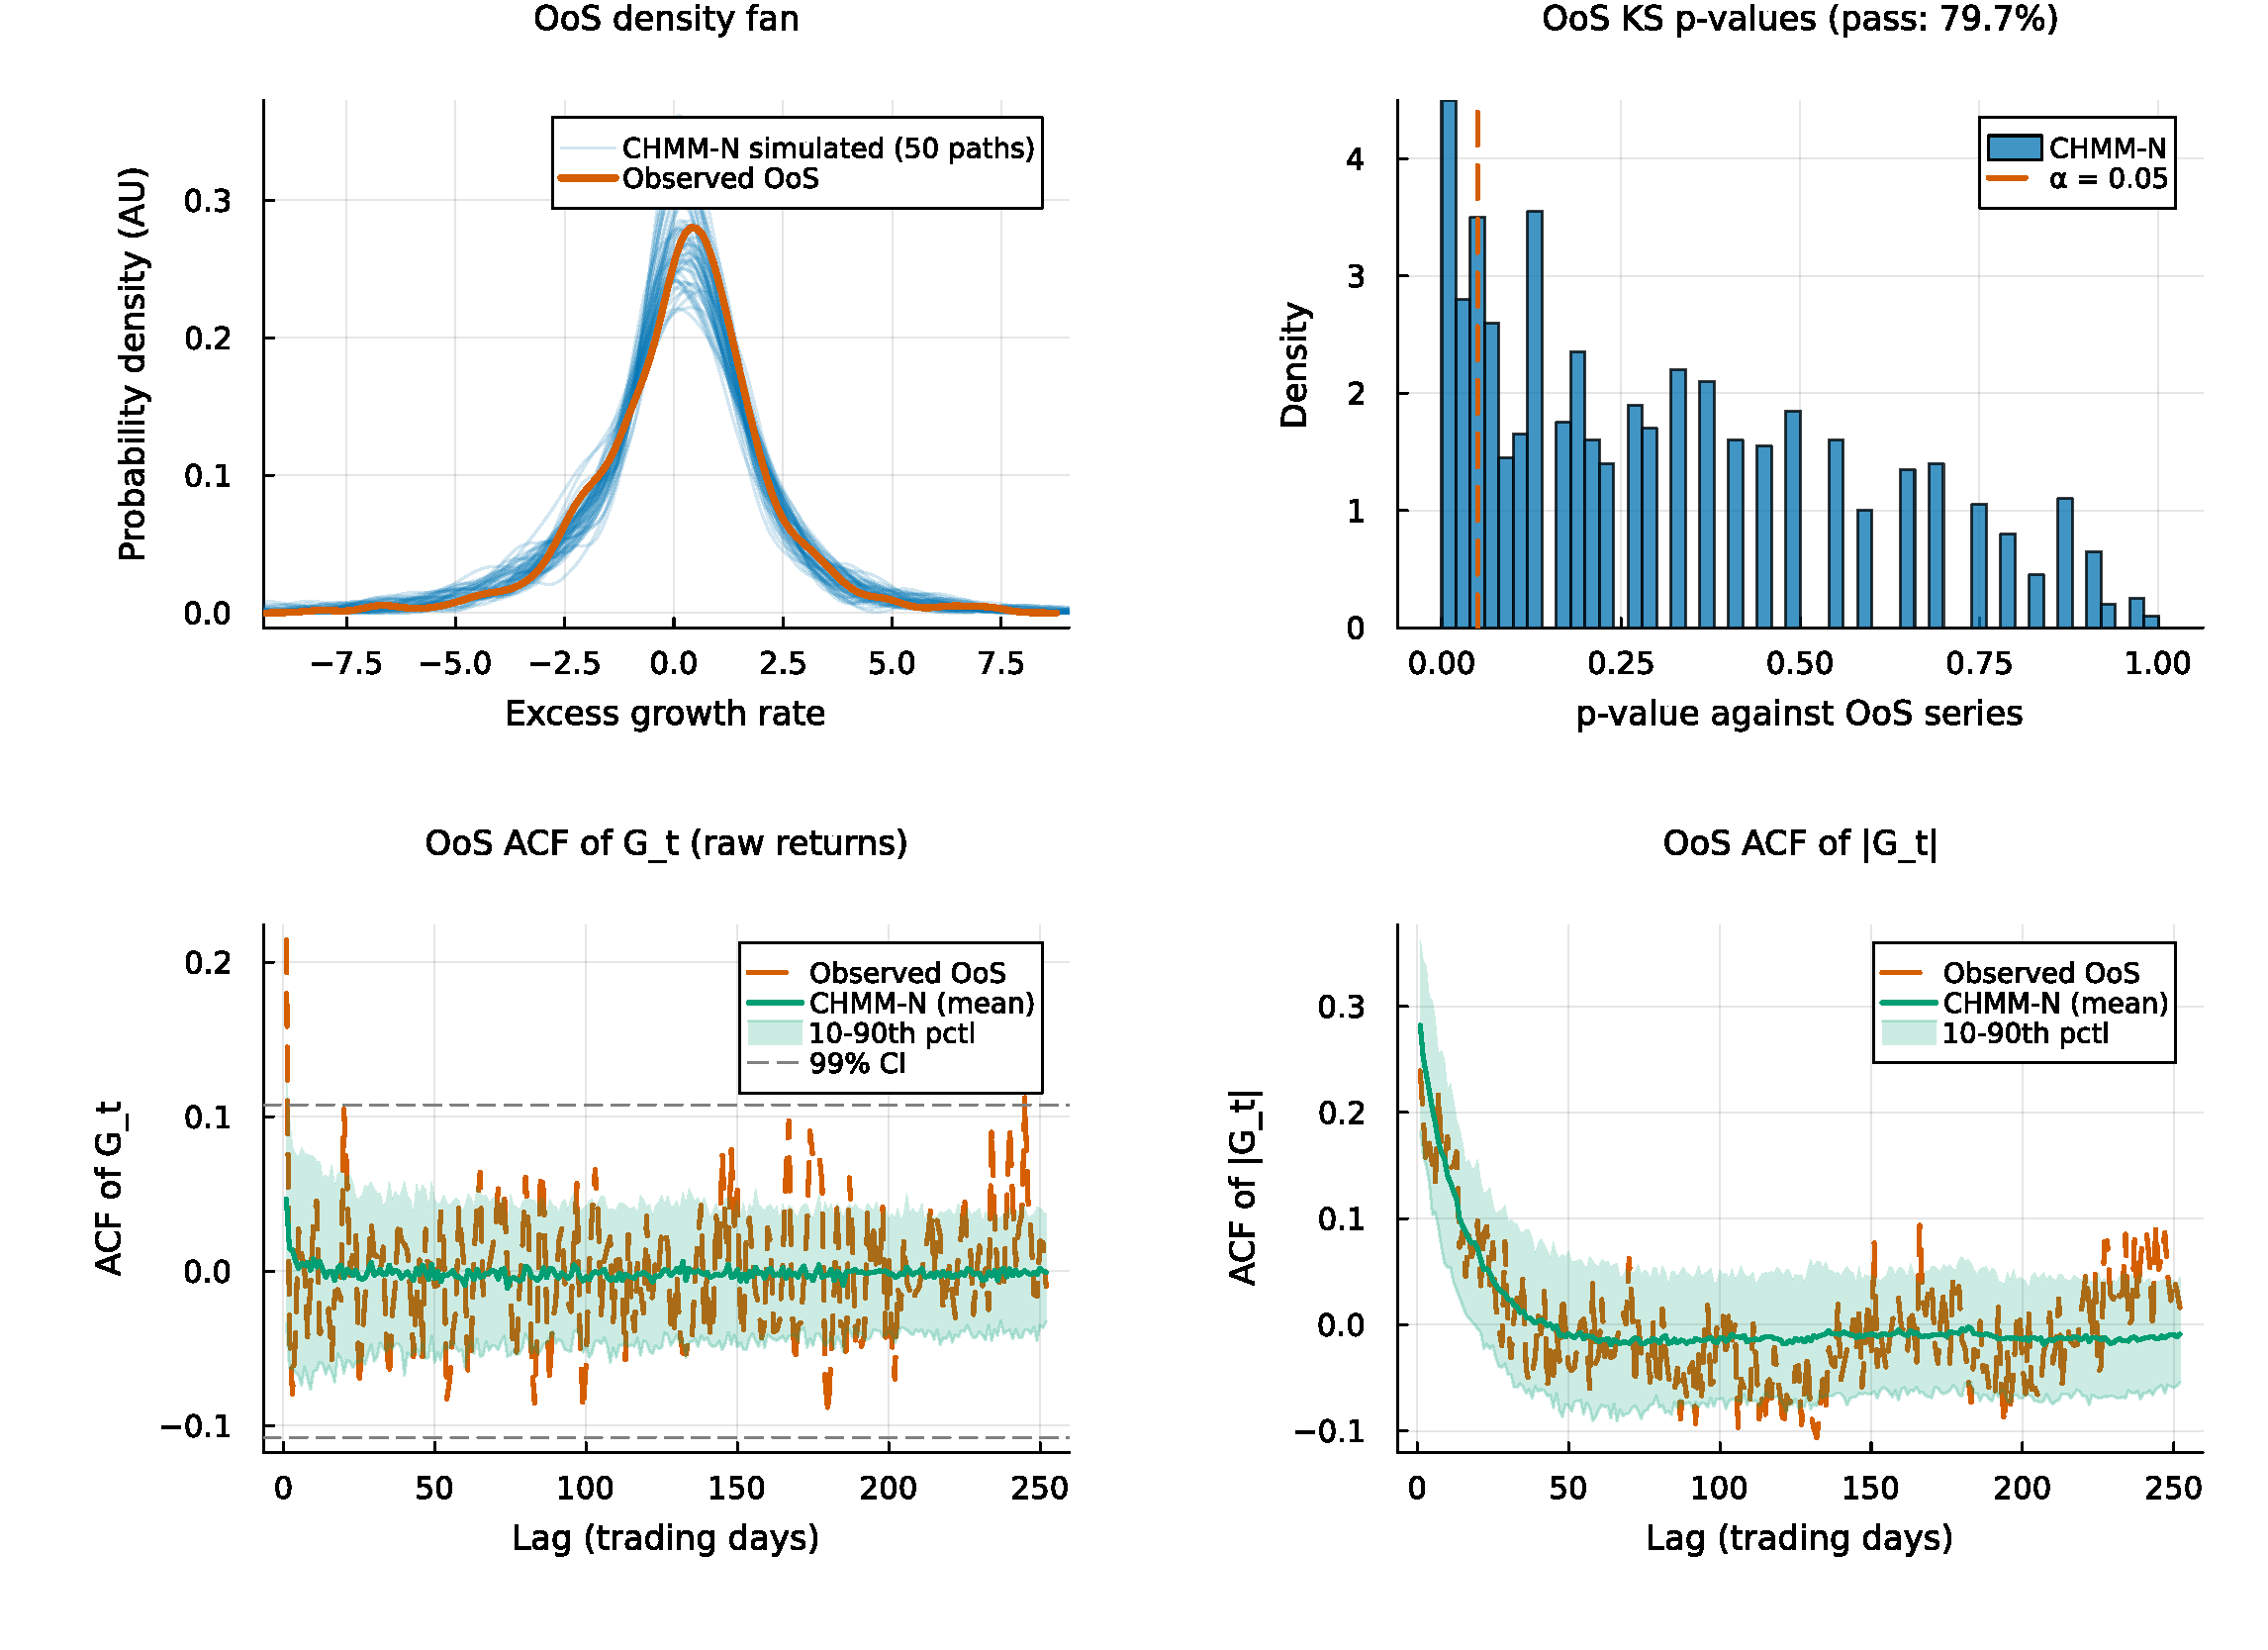
\includegraphics[width=\textwidth]{figs/Fig-4-OoS-Validation-K6.pdf}
\caption{OoS SPY CHMM-N validation at $K = 6$ (Pipeline~A, 1{,}000 simulated paths; panels as in Figure~\ref{fig:oos_validation}).}
\label{fig:k_sweep_oos_k6}
\end{figure}

\begin{figure}[H]
\centering
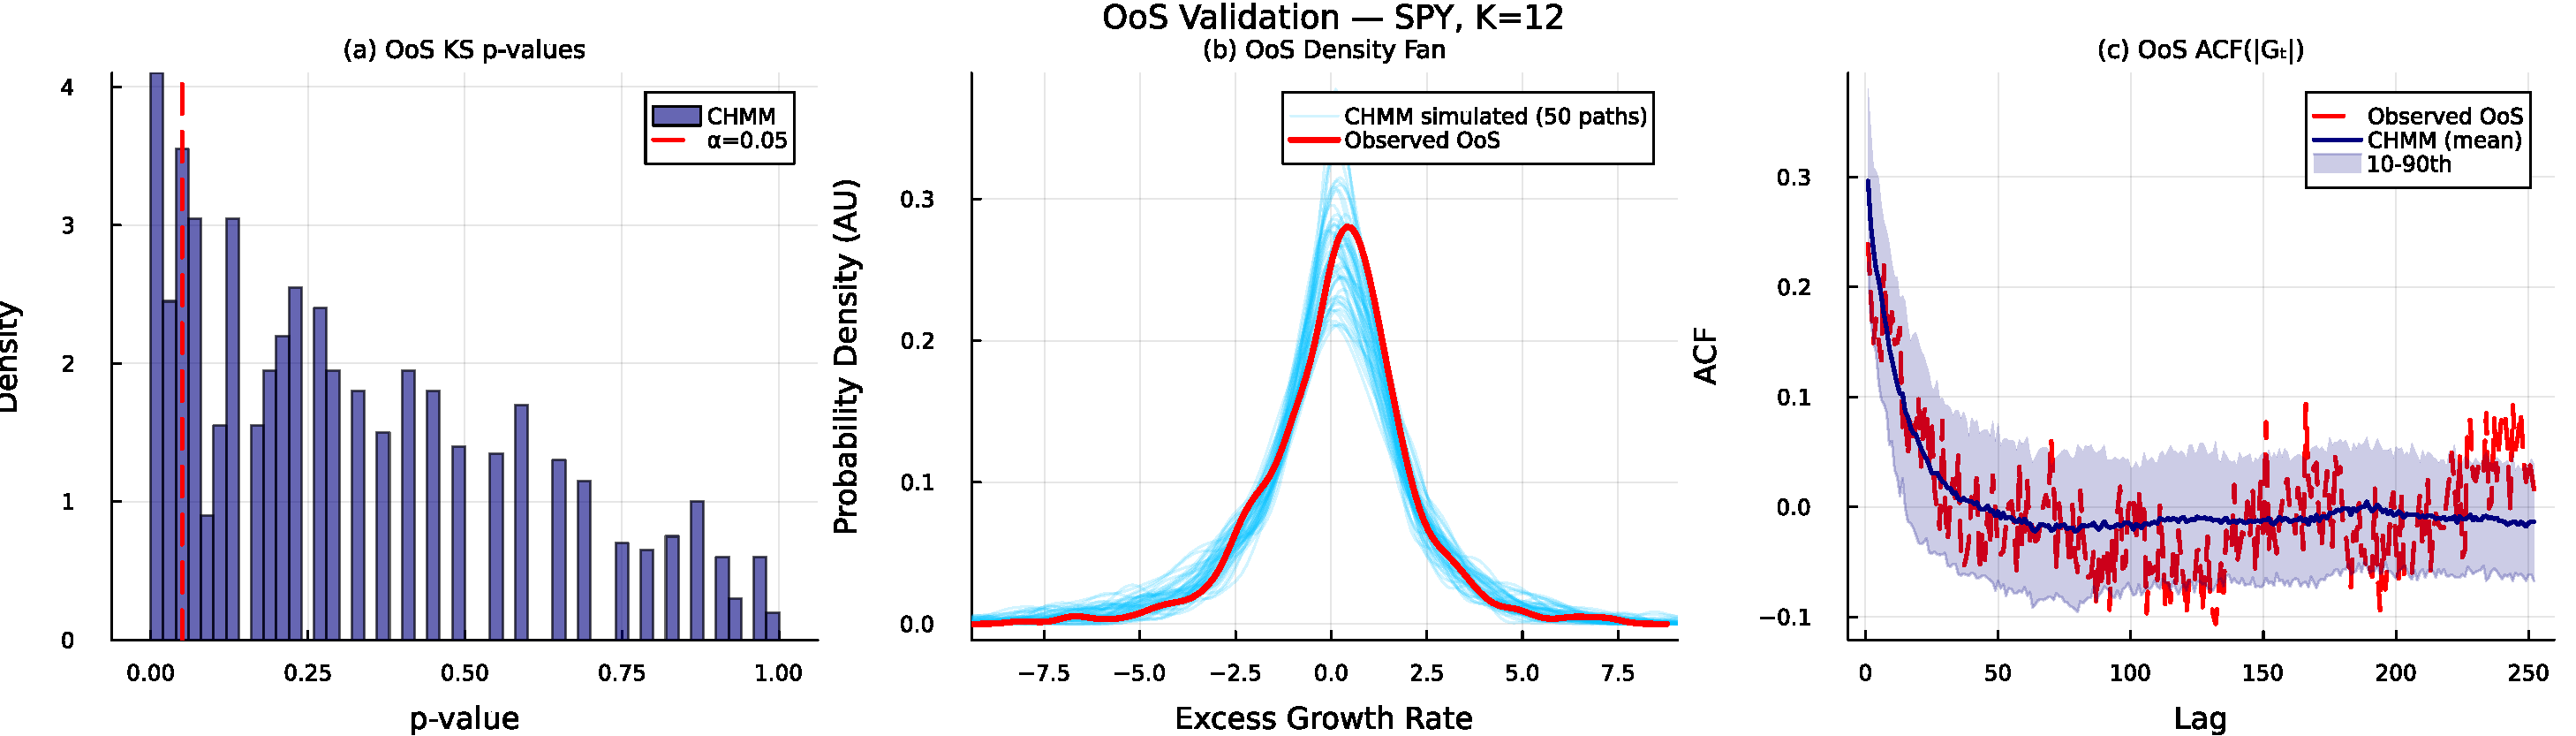
\includegraphics[width=\textwidth]{figs/Fig-4-OoS-Validation-K12.pdf}
\caption{OoS SPY CHMM-N validation at $K = 12$ (Pipeline~A, 1{,}000 simulated paths; panels as in Figure~\ref{fig:oos_validation}).}
\label{fig:k_sweep_oos_k12}
\end{figure}

\begin{figure}[H]
\centering
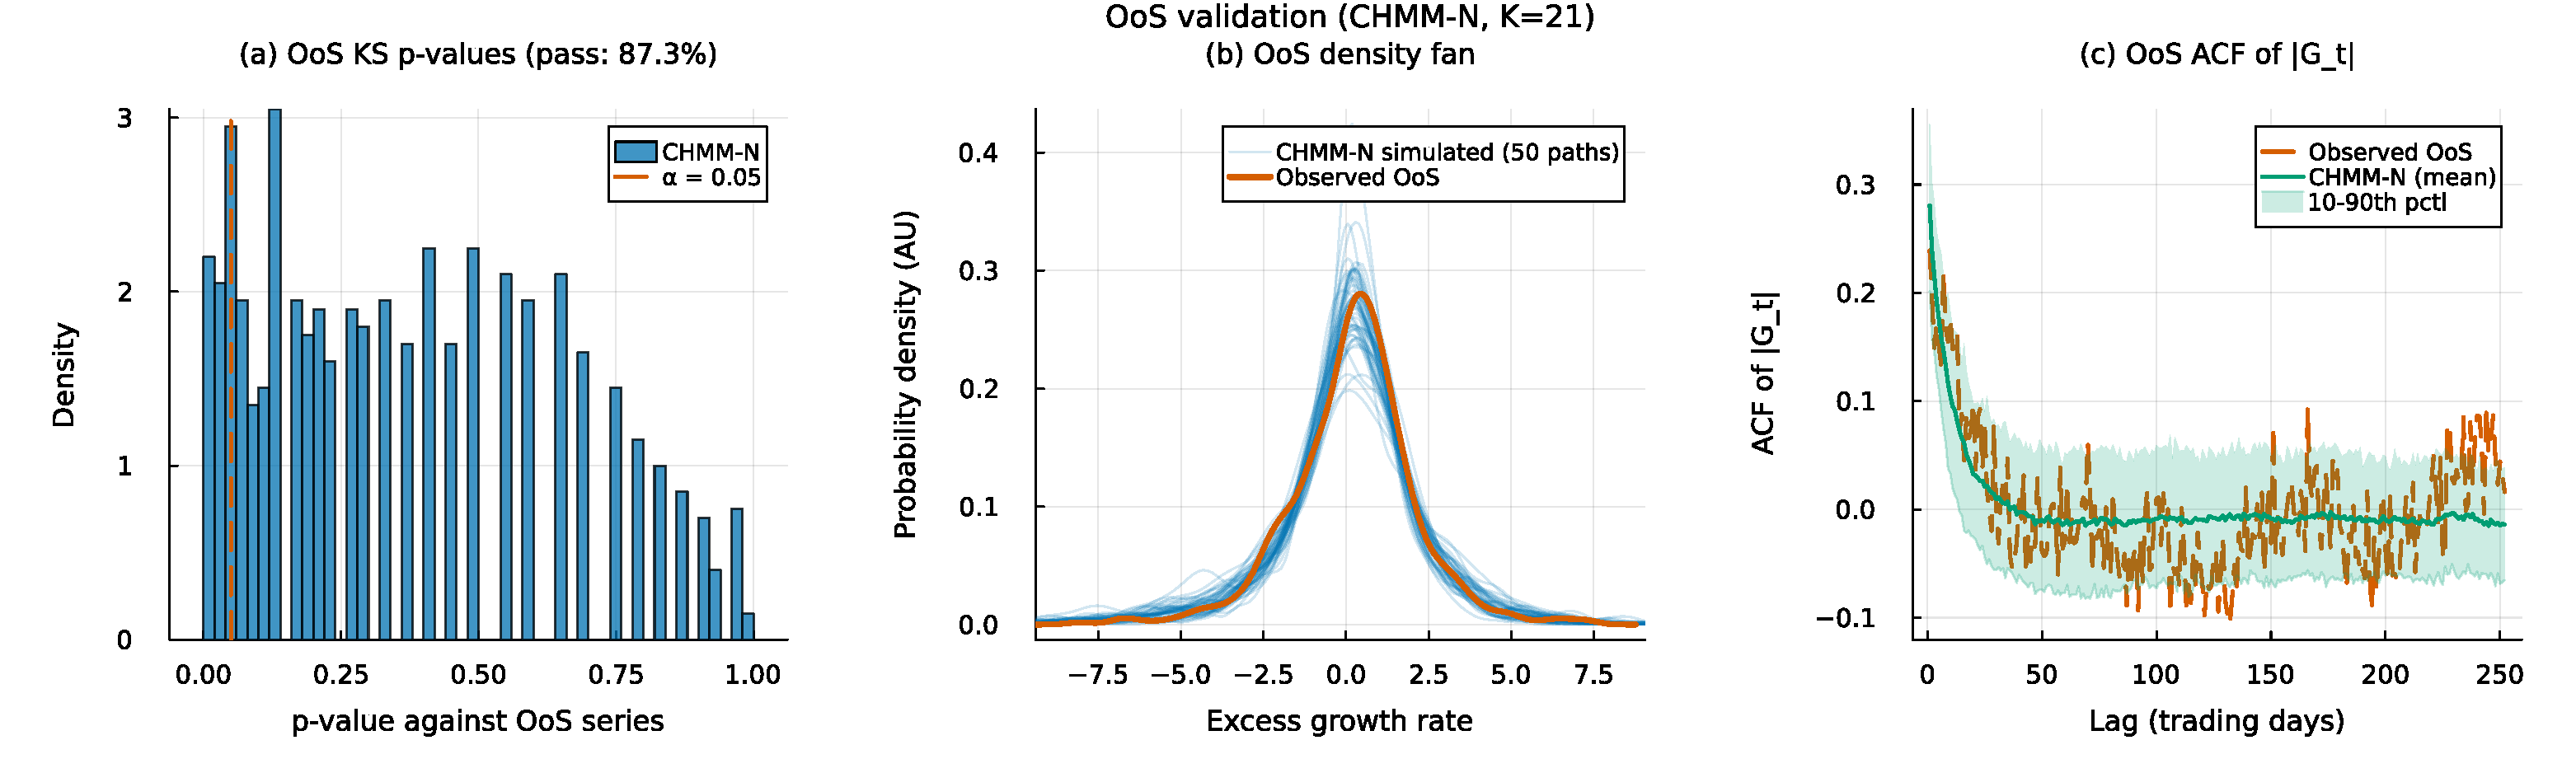
\includegraphics[width=\textwidth]{figs/Fig-4-OoS-Validation-K21.pdf}
\caption{OoS SPY CHMM-N validation at $K = 21$ (Pipeline~A, 1{,}000 simulated paths; panels as in Figure~\ref{fig:oos_validation}).}
\label{fig:k_sweep_oos_k21}
\end{figure}

\subsubsection{\texorpdfstring{Multi-Emission Figures at $K = 18$}{Multi-Emission Figures at K = 18}}
\label{sec:multi_emission_figs}

This appendix reproduces the standard diagnostic suite (emission PDFs, residence times, IS comparison, OoS validation, and convergence) for the two heavy-tailed emission families (CHMM-t and CHMM-L) at the selected state resolution $K = 18$; transition matrices and stationary distributions are discussed in prose only below, since they are visually indistinguishable across families at $K = 18$.
The Gaussian counterparts are already shown as Figures~\ref{fig:is_comparison} and~\ref{fig:oos_validation} in the main text and as Figure~\ref{fig:convergence_all} above in this appendix.
The figures confirm that the shared forward--backward scaffold produces internally-similar regime structure across the three families: the near-diagonal transition band, the $K$-component dense emission cover, the longer central-state residence times, and the monotone log-likelihood convergence are features of the CHMM framework and not of the Gaussian component specifically.

\paragraph{Emission PDFs.}
Figure~\ref{fig:emissions_families} compares the learned $K = 18$ emissions for the three families.
The CHMM-t panel's per-state $\nu_k$ allocation is visible in the narrower modes of certain tail states; the CHMM-L panel's Laplace components have sharper peaks and slower exponential tail decay than the Gaussians.

\begin{figure}[H]
\centering
\begin{subfigure}[b]{0.32\textwidth}
    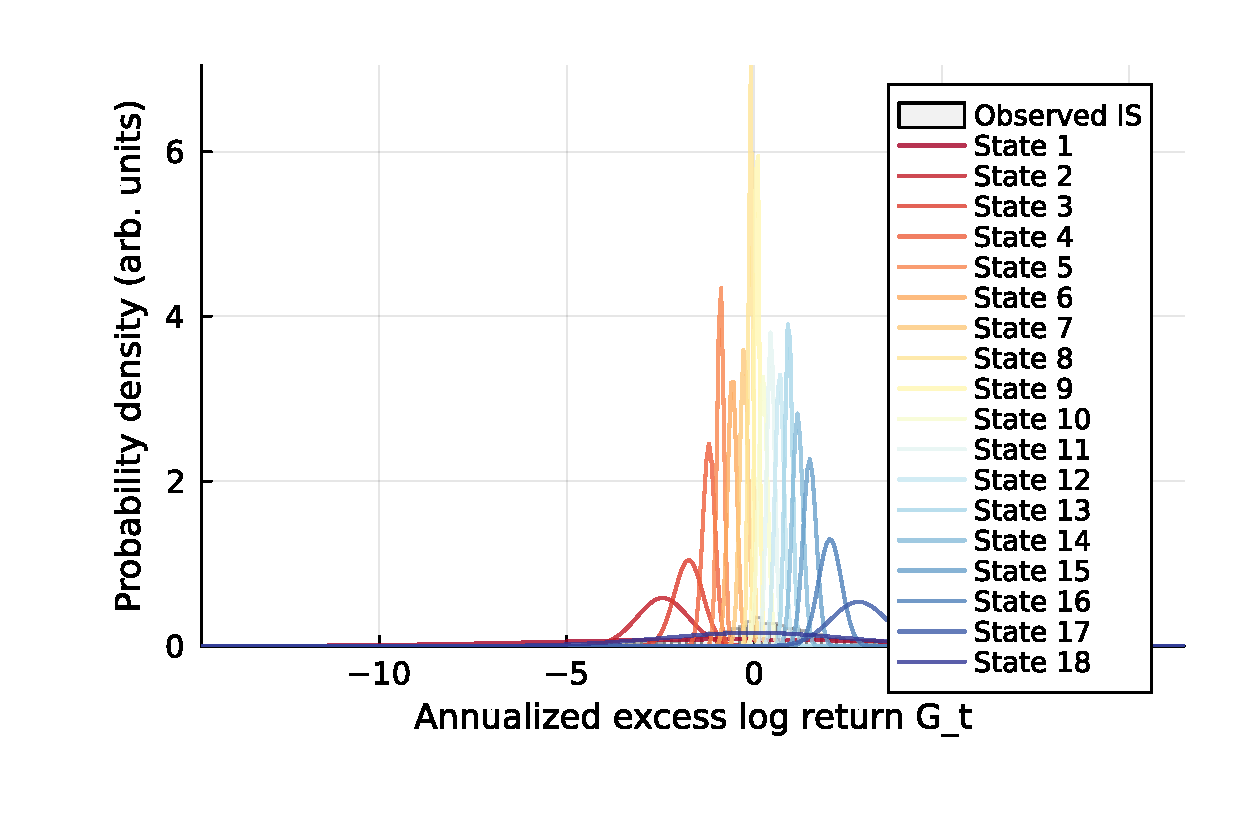
\includegraphics[width=\textwidth]{figs/Fig-Emission-PDFs-K18-N.pdf}
    \caption{CHMM-N (Gaussian)}
\end{subfigure}
\hfill
\begin{subfigure}[b]{0.32\textwidth}
    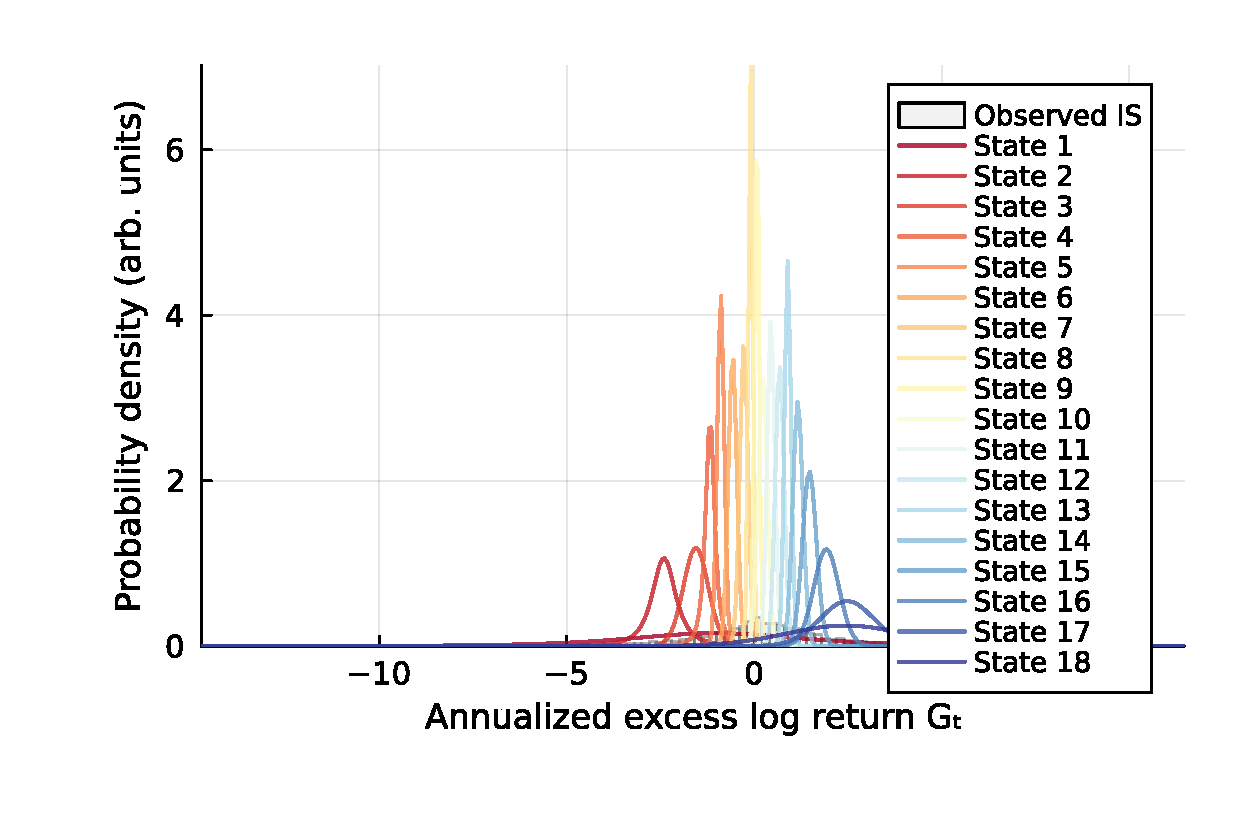
\includegraphics[width=\textwidth]{figs/Fig-Emission-PDFs-K18-t.pdf}
    \caption{CHMM-t (Student-t)}
\end{subfigure}
\hfill
\begin{subfigure}[b]{0.32\textwidth}
    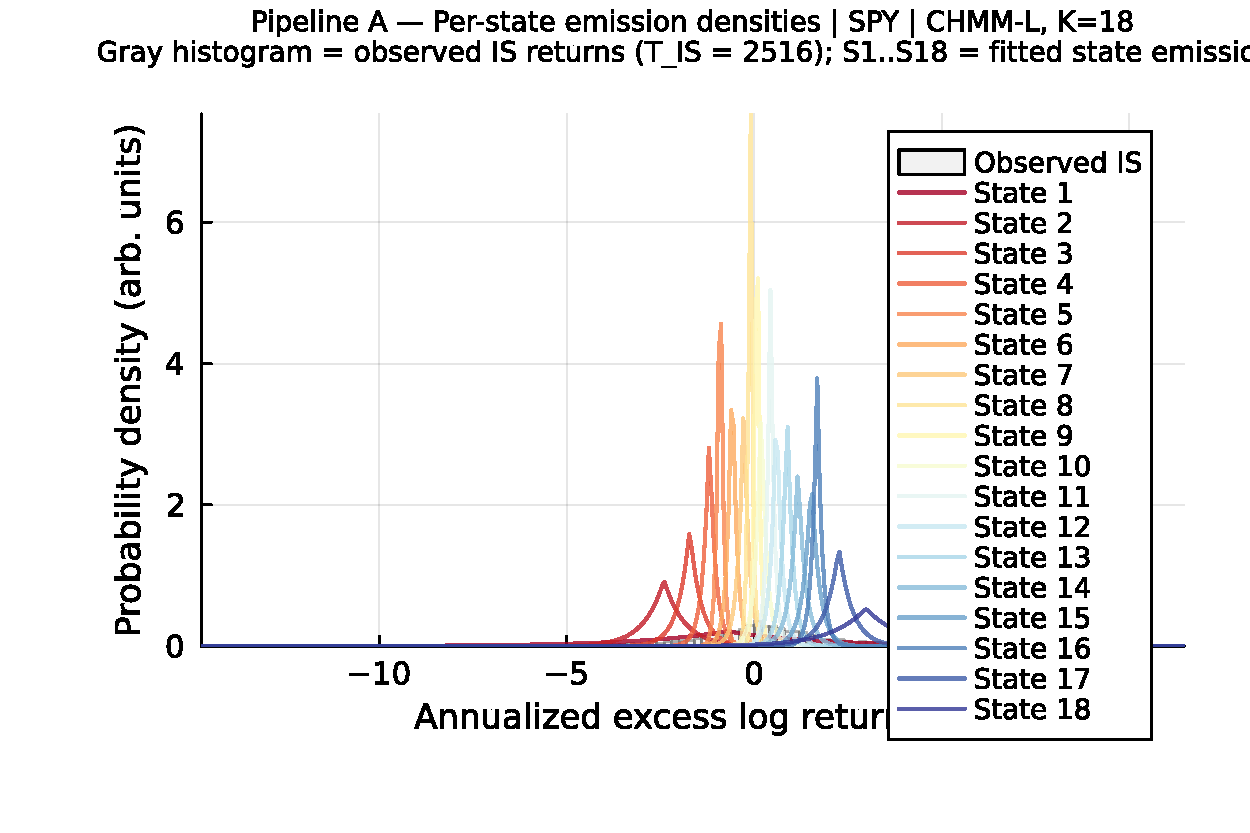
\includegraphics[width=\textwidth]{figs/Fig-Emission-PDFs-K18-L.pdf}
    \caption{CHMM-L (Laplace)}
\end{subfigure}
\caption{Learned emission distributions at $K = 18$ across the three emission families (CHMM-N Gaussian, CHMM-t Student-t with per-state $\nu_k$, CHMM-L Laplace), overlaid on the observed SPY IS return histogram (Pipeline~A). Heavier-tailed emission families (t, L) give individual components more tail mass, which is what closes the kurtosis gap of the Gaussian CHMM.}
\label{fig:emissions_families}
\end{figure}

\paragraph{Transition matrices and stationary distributions.}
The $K = 18$ transition matrices and stationary distributions learned under CHMM-t and CHMM-L are visually indistinguishable from their CHMM-N counterparts: the near-diagonal band, the magnitude of self-transition probabilities, and the mass concentration at central states are features of the regime structure, not the emission family. This is consistent with the ACF-MAE being stable across the family axis (Table~\ref{tab:sensitivity_multi}). The per-family residence times $\tau_k = 1/(1 - T_{kk})$, which magnify small differences in the self-transition probabilities each family recovers, are compared in Figure~\ref{fig:residence_families}.

\begin{figure}[H]
\centering
\begin{subfigure}[b]{0.32\textwidth}
    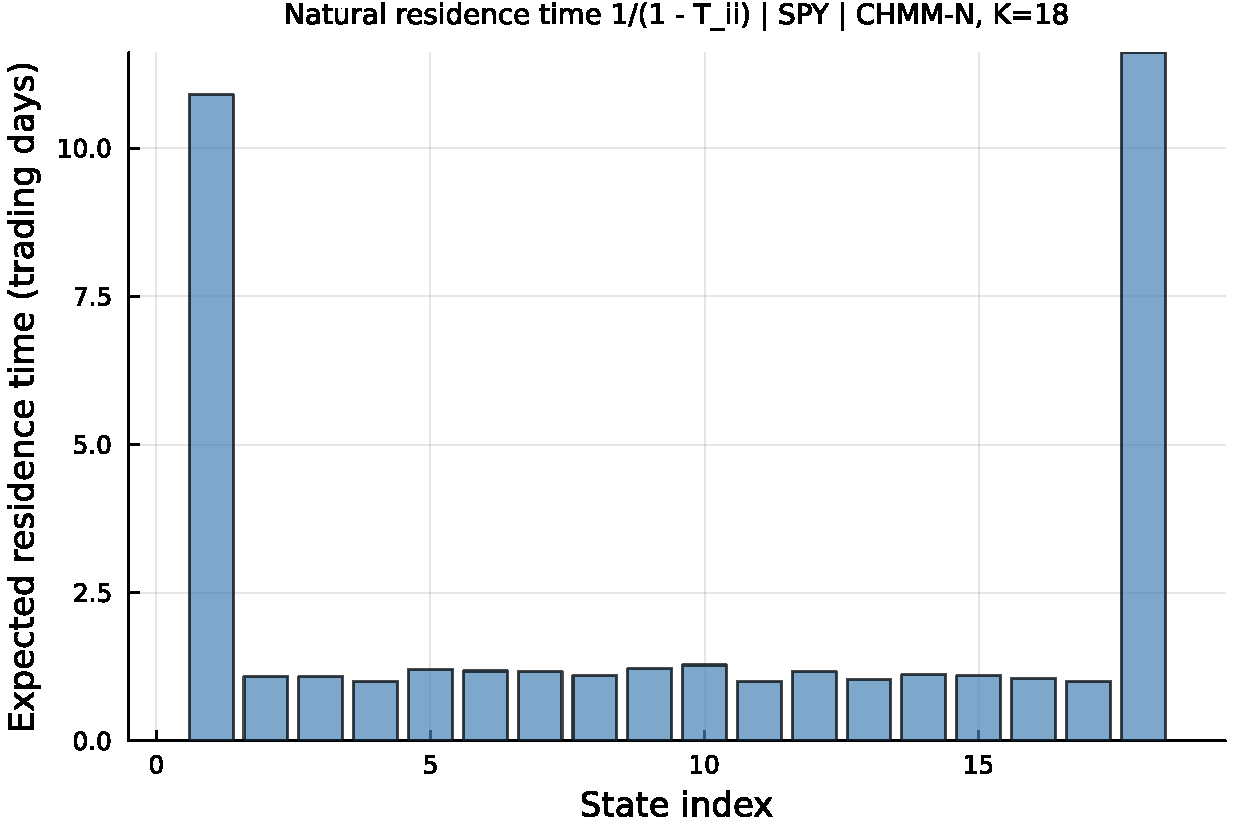
\includegraphics[width=\textwidth]{figs/Fig-Residence-Times-K18-N.pdf}
    \caption{CHMM-N}
\end{subfigure}
\hfill
\begin{subfigure}[b]{0.32\textwidth}
    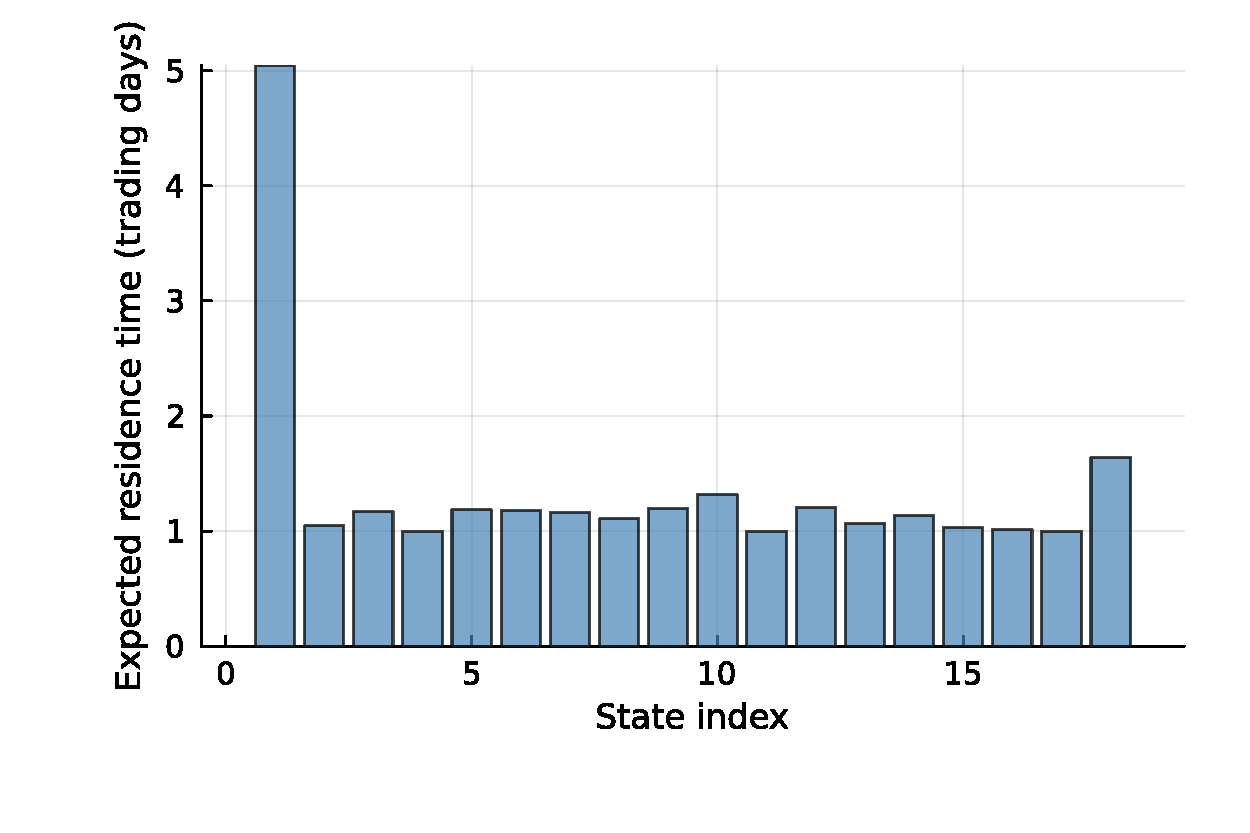
\includegraphics[width=\textwidth]{figs/Fig-Residence-Times-K18-t.pdf}
    \caption{CHMM-t}
\end{subfigure}
\hfill
\begin{subfigure}[b]{0.32\textwidth}
    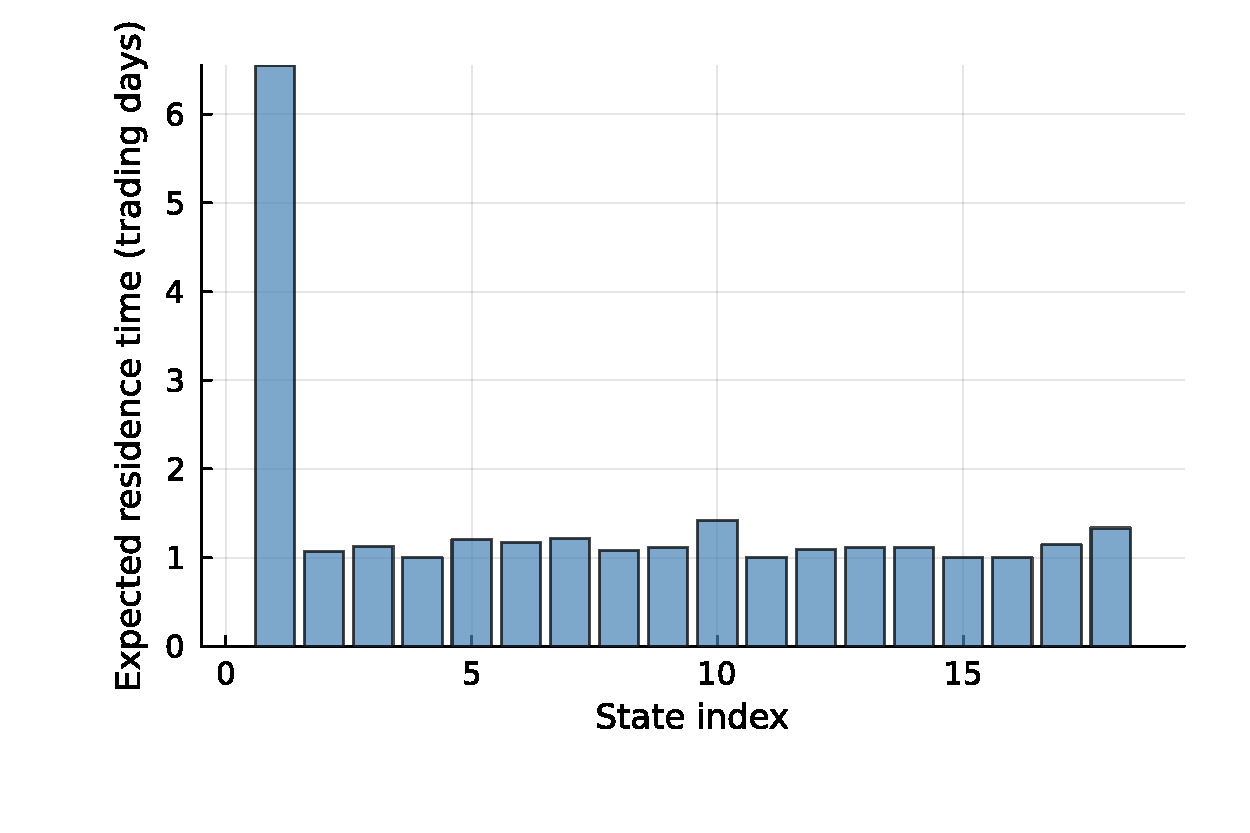
\includegraphics[width=\textwidth]{figs/Fig-Residence-Times-K18-L.pdf}
    \caption{CHMM-L}
\end{subfigure}
\caption{Natural residence times $\tau_k = 1/(1 - T_{kk})$ at $K = 18$ for the SPY IS fit (Pipeline~A) across the three emission families (CHMM-N Gaussian, CHMM-t Student-t, CHMM-L Laplace).}
\label{fig:residence_families}
\end{figure}

\paragraph{IS comparison.}
Figures~\ref{fig:is_families}--\ref{fig:is_families_L} reproduce the three-panel IS comparison (density, ACF of $|G_t|$, tail Q-Q) at $K = 18$ for the two heavy-tailed families; the CHMM-N panel is Figure~\ref{fig:is_comparison} in the main text.

\begin{figure}[H]
\centering
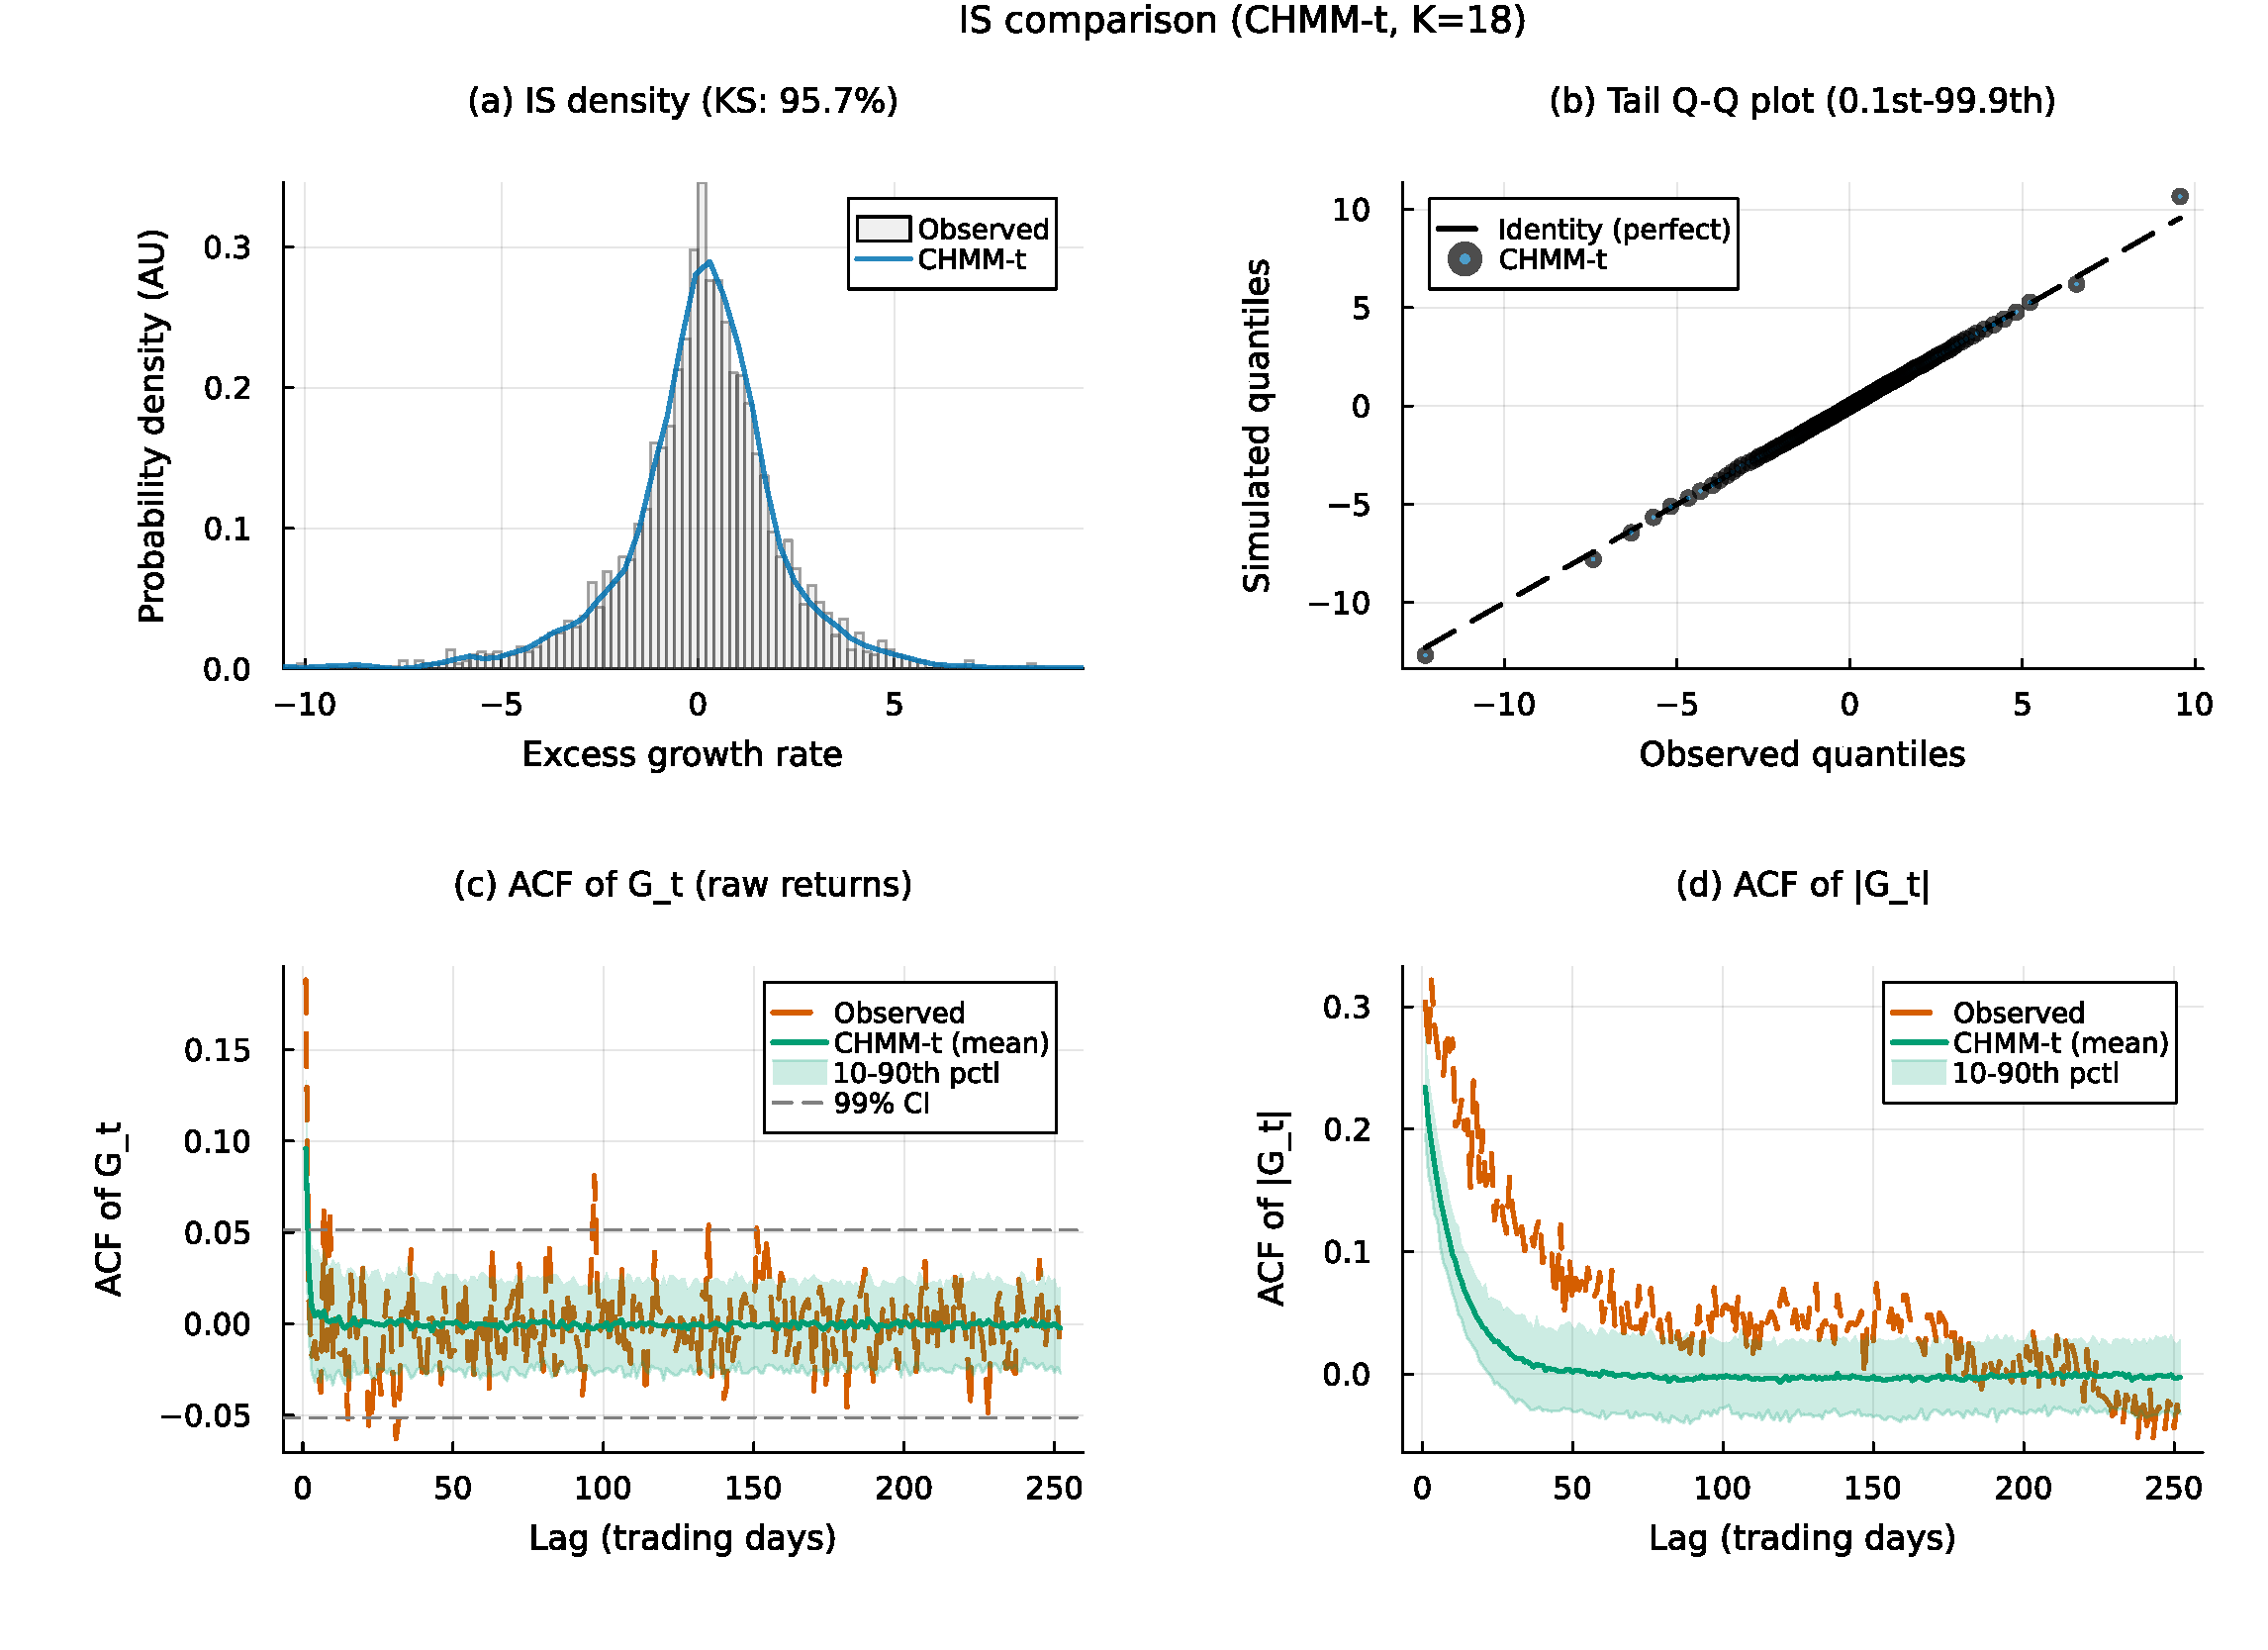
\includegraphics[width=\textwidth]{figs/Fig-3-IS-Comparison-K18-t.pdf}
\caption{IS SPY model comparison at $K = 18$ for CHMM-t Student-t emissions (Pipeline~A, 1{,}000 simulated paths). Panels show (a) marginal density with KS pass rate, (b) ACF of $|G_t|$, and (c) tail Q-Q plot. The CHMM-N counterpart is Figure~\ref{fig:is_comparison}; the CHMM-L counterpart is Figure~\ref{fig:is_families_L}.}
\label{fig:is_families}
\end{figure}

\begin{figure}[H]
\centering
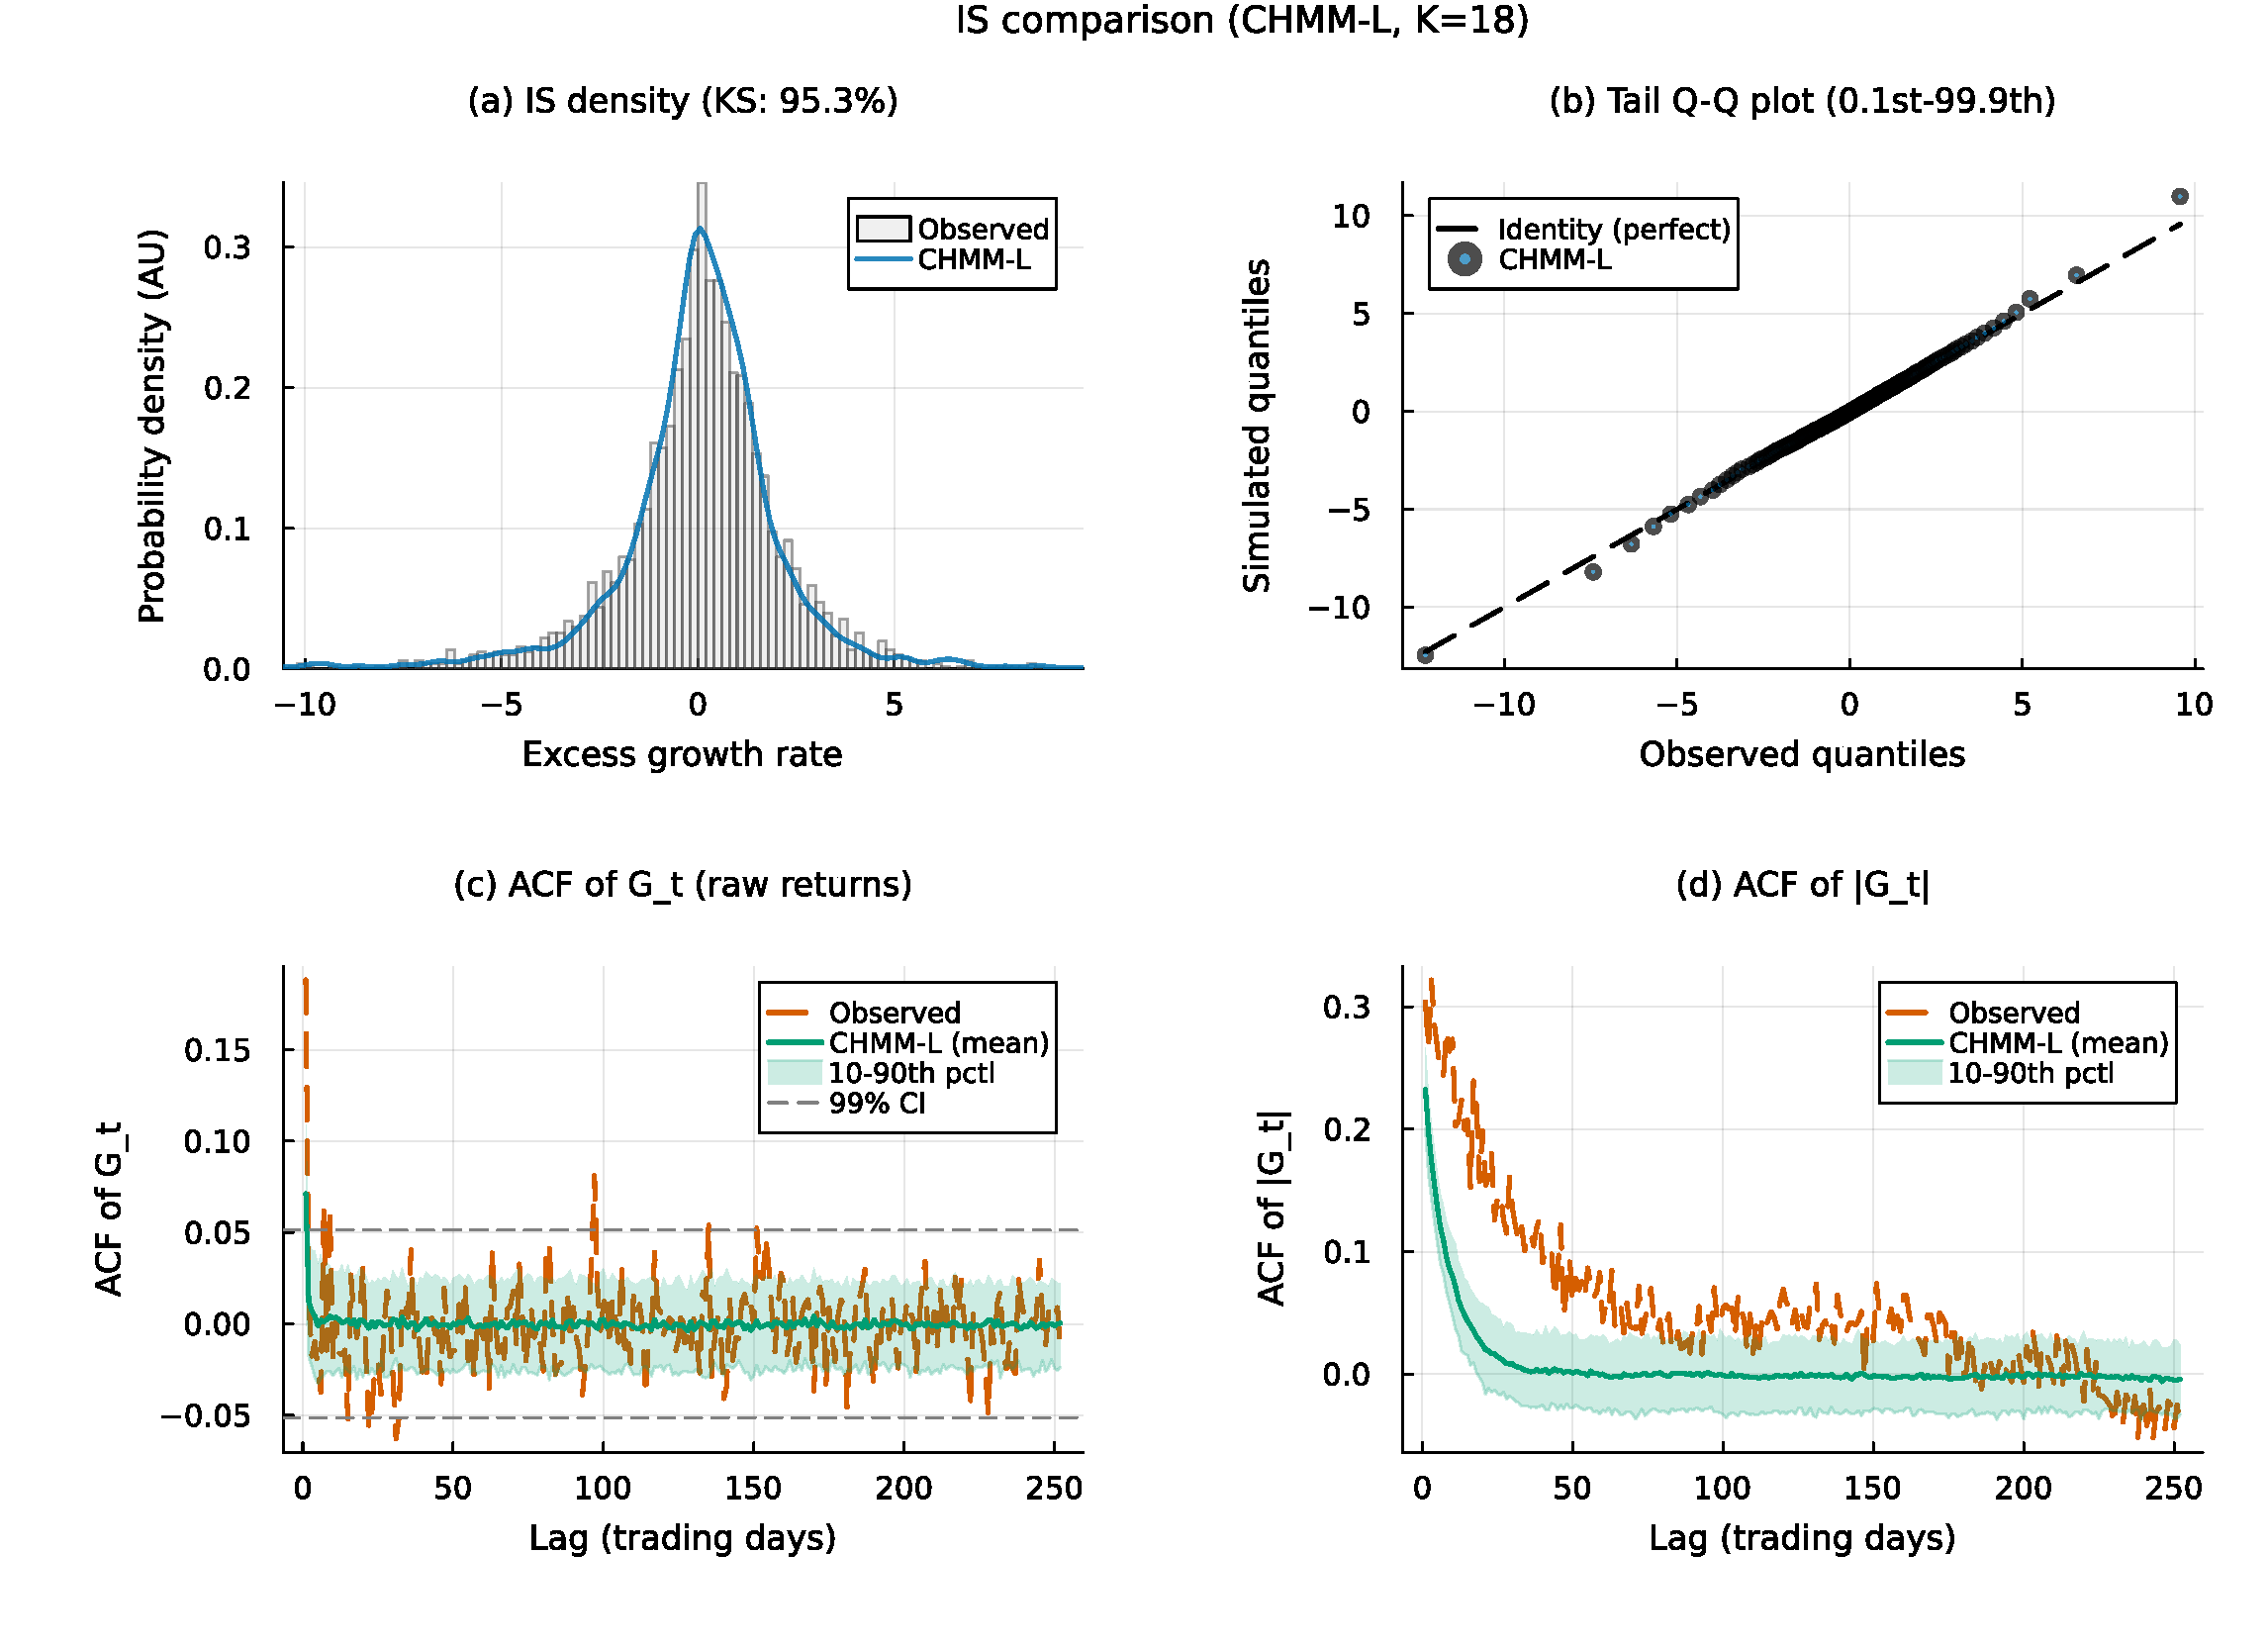
\includegraphics[width=\textwidth]{figs/Fig-3-IS-Comparison-K18-L.pdf}
\caption{IS SPY model comparison at $K = 18$ for CHMM-L Laplace emissions (Pipeline~A, 1{,}000 simulated paths). Panels as in Figure~\ref{fig:is_families}.}
\label{fig:is_families_L}
\end{figure}

\paragraph{OoS validation.}
Figures~\ref{fig:oos_families}--\ref{fig:oos_families_L} show the OoS validation panels for CHMM-t and CHMM-L at $K = 18$.
The CHMM-t panel demonstrates the OoS kurtosis alignment noted in the main text (simulated 6.40 vs.\ observed 6.24), and the CHMM-L panel shows the tighter density fan produced by the heavier Laplace tails relative to the Gaussian.

\begin{figure}[H]
\centering
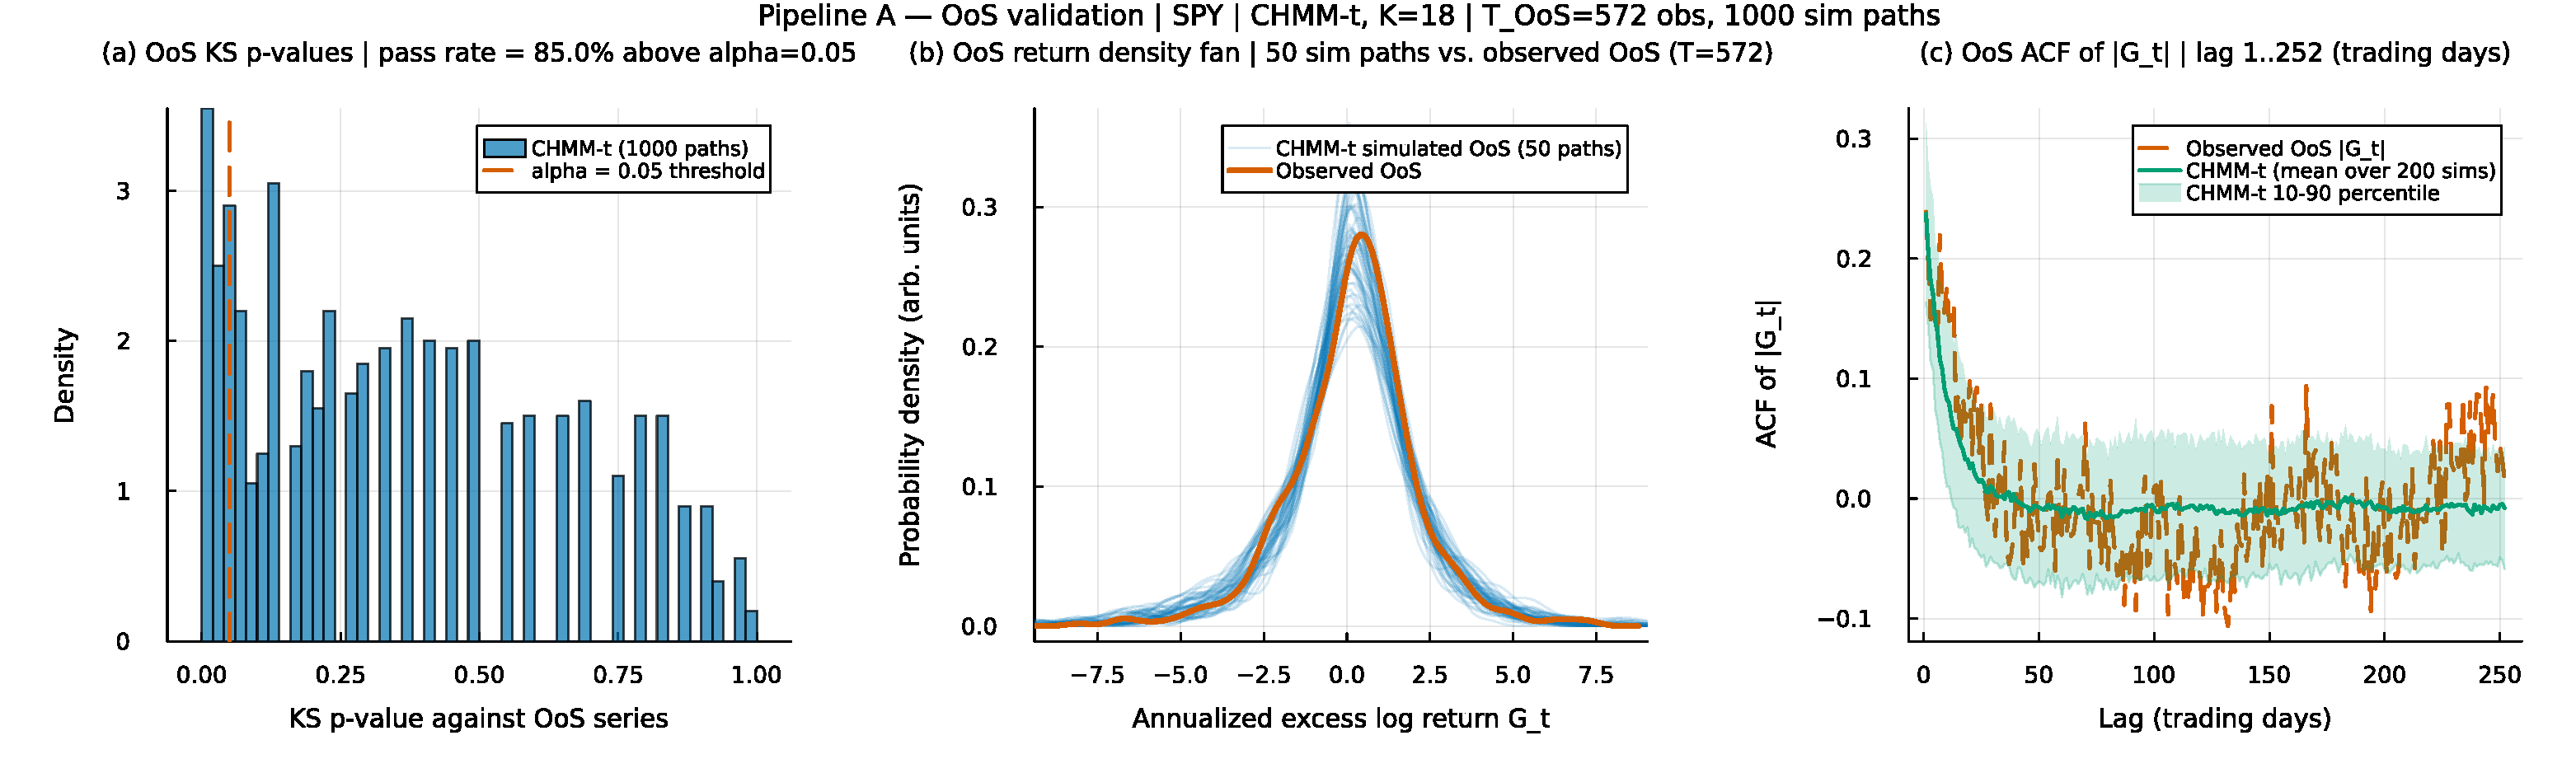
\includegraphics[width=\textwidth]{figs/Fig-4-OoS-Validation-K18-t.pdf}
\caption{OoS SPY validation at $K = 18$ for CHMM-t Student-t emissions (Pipeline~A, 1{,}000 simulated paths). Panels show (a) KS $p$-values, (b) OoS density fan, and (c) OoS ACF of $|G_t|$. The CHMM-N counterpart is Figure~\ref{fig:oos_validation}; the CHMM-L counterpart is Figure~\ref{fig:oos_families_L}.}
\label{fig:oos_families}
\end{figure}

\begin{figure}[H]
\centering
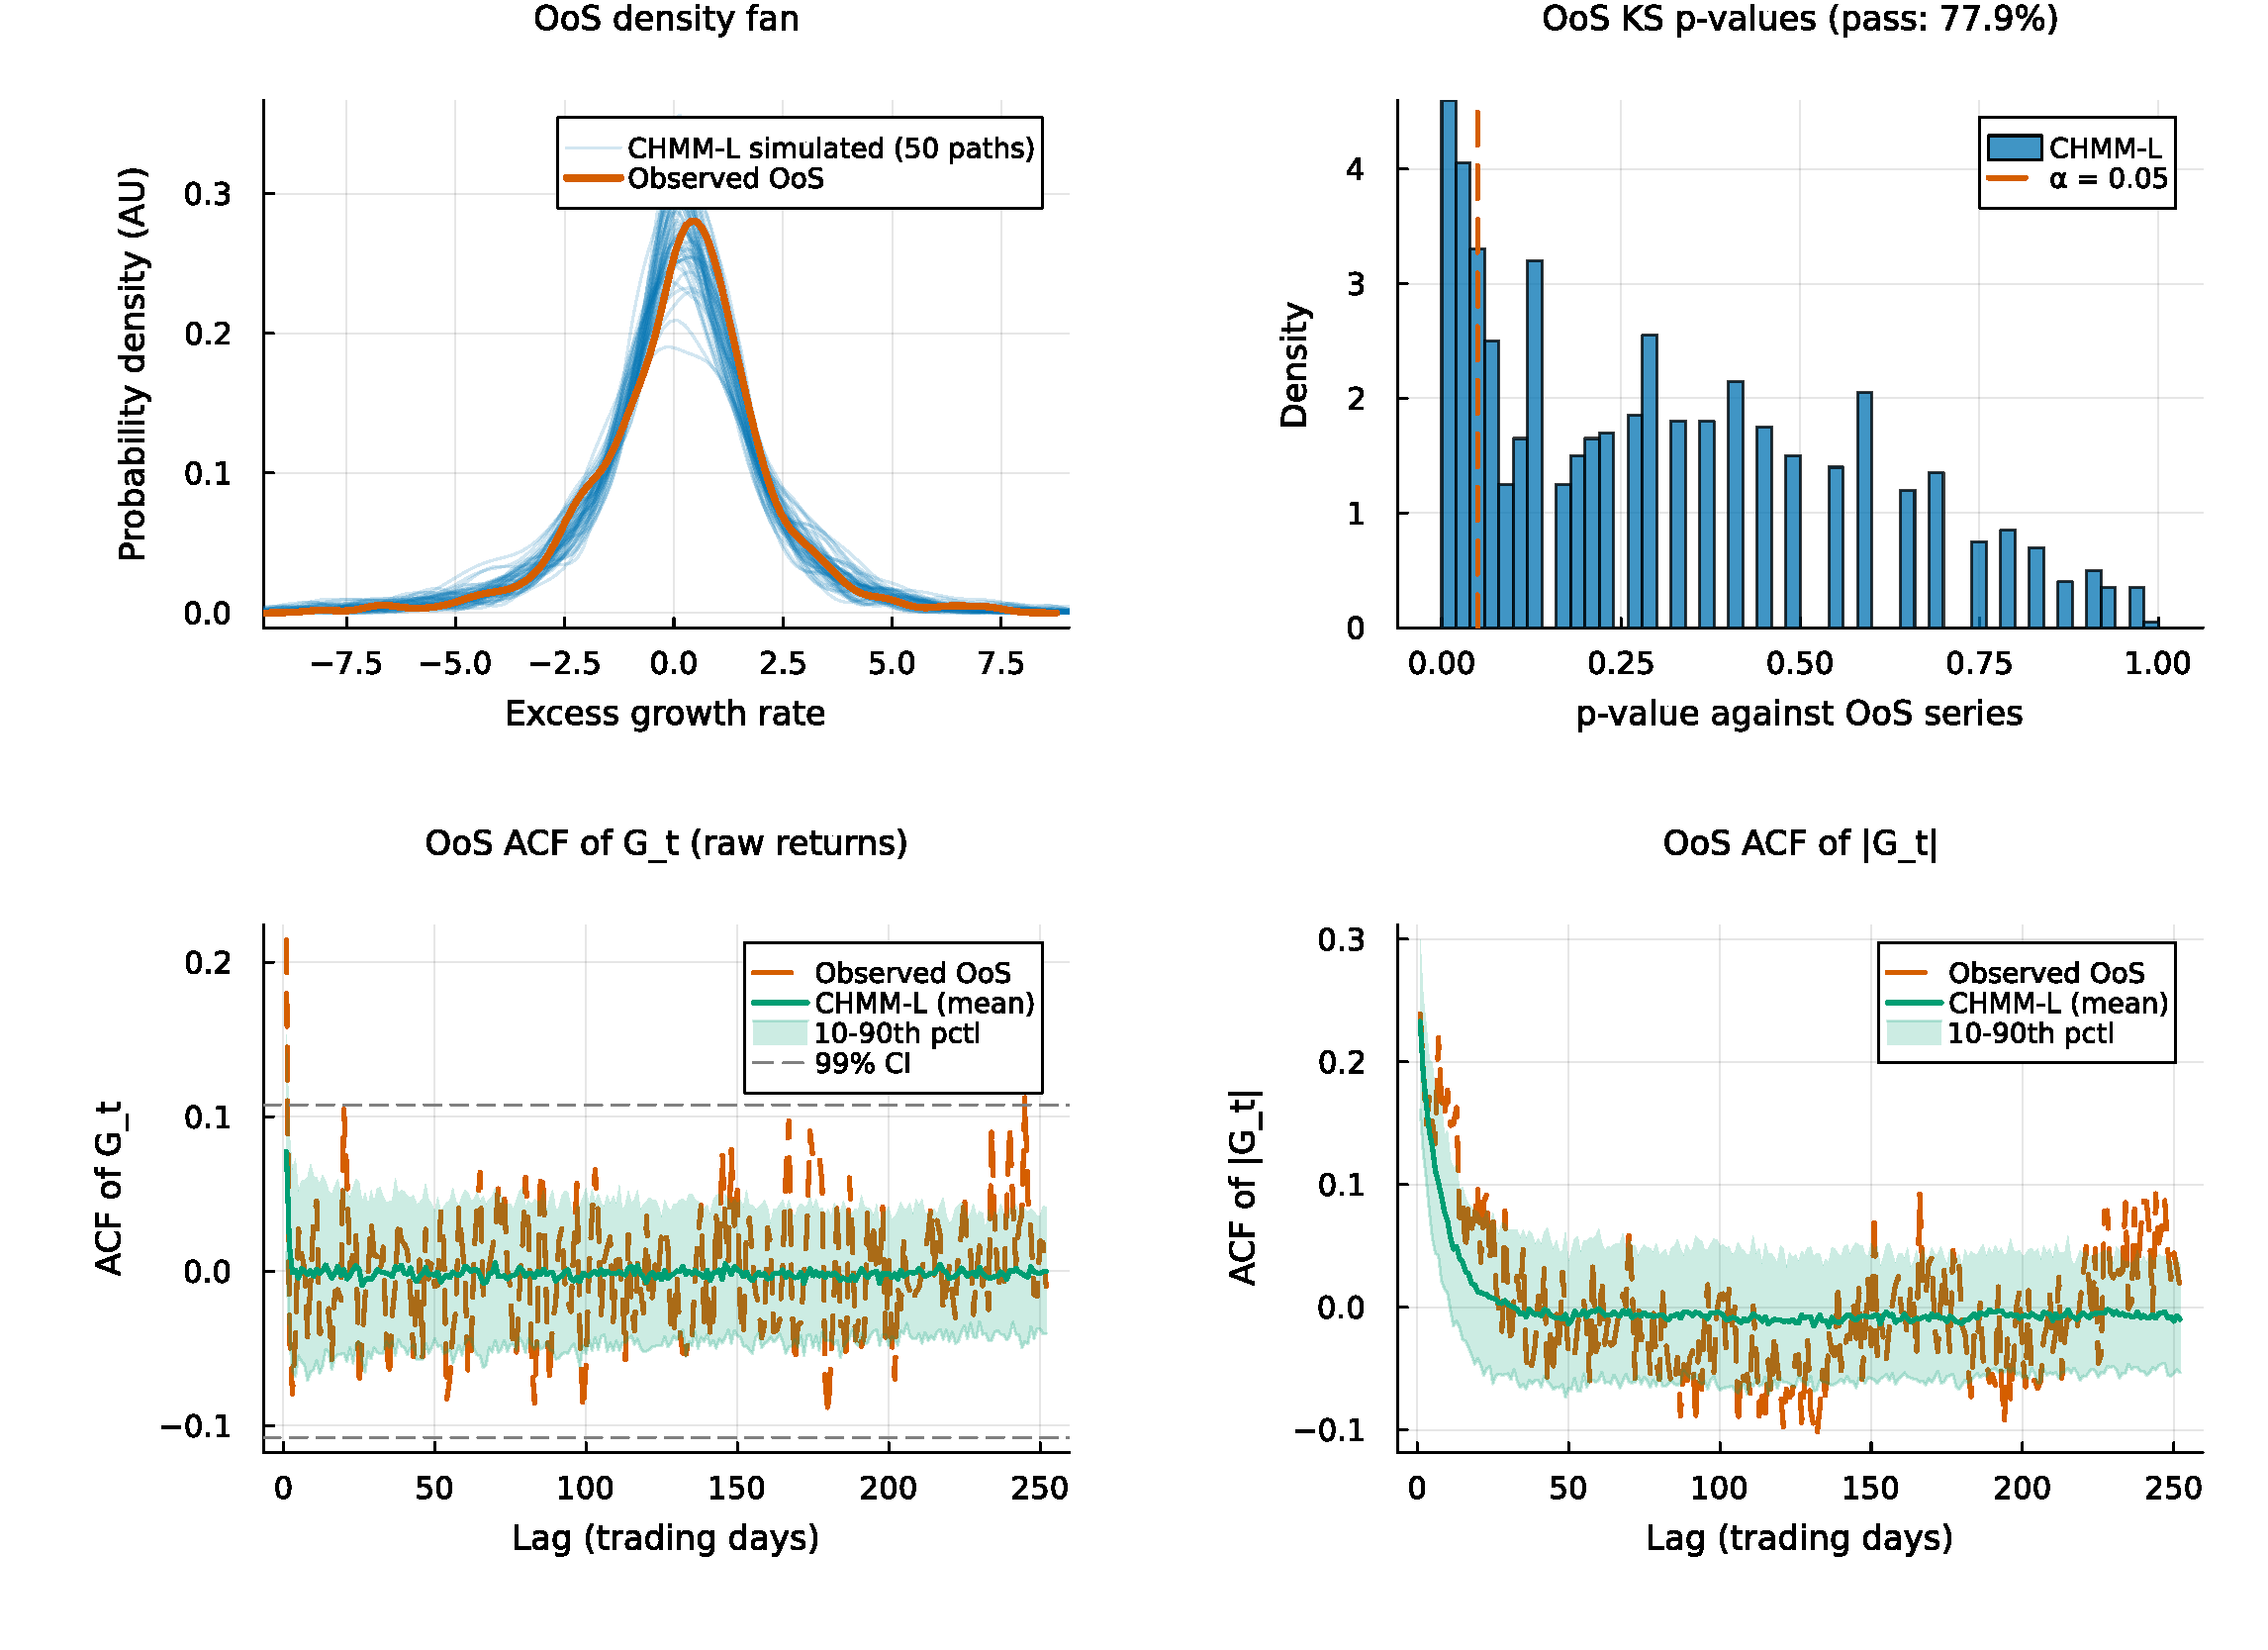
\includegraphics[width=\textwidth]{figs/Fig-4-OoS-Validation-K18-L.pdf}
\caption{OoS SPY validation at $K = 18$ for CHMM-L Laplace emissions (Pipeline~A, 1{,}000 simulated paths). Panels as in Figure~\ref{fig:oos_families}.}
\label{fig:oos_families_L}
\end{figure}

\paragraph{Convergence.}
Figure~\ref{fig:convergence_families} shows the Baum-Welch / ECM / weighted-EM log-likelihood histories at $K = 18$ for all three families.
The CHMM-t and CHMM-L curves inherit the monotone increase of the classical EM guarantee; the CHMM-t curve has a slightly longer pre-plateau phase because each ECM sub-iteration refines $\nu_k$ with a golden-section search.

\begin{figure}[H]
\centering
\begin{subfigure}[b]{0.32\textwidth}
    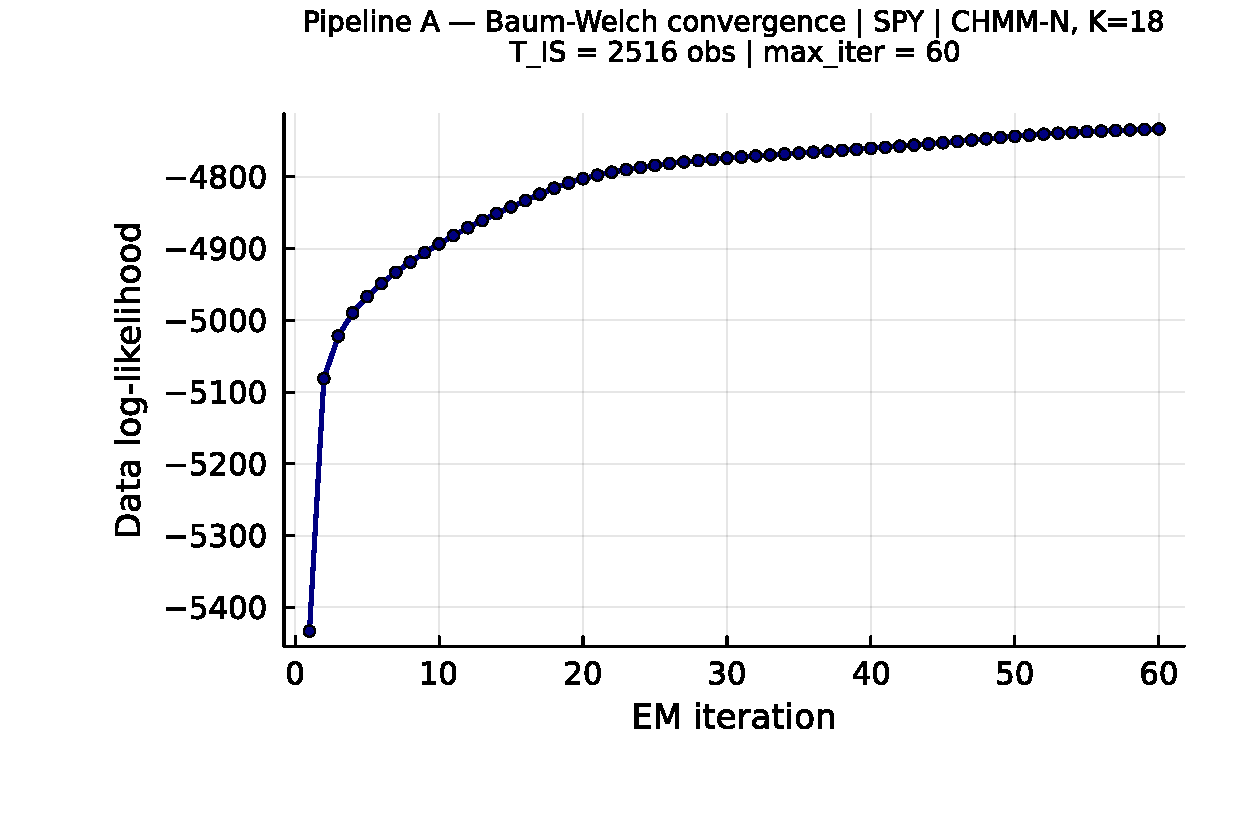
\includegraphics[width=\textwidth]{figs/Fig-Convergence-K18-N.pdf}
    \caption{CHMM-N}
\end{subfigure}
\hfill
\begin{subfigure}[b]{0.32\textwidth}
    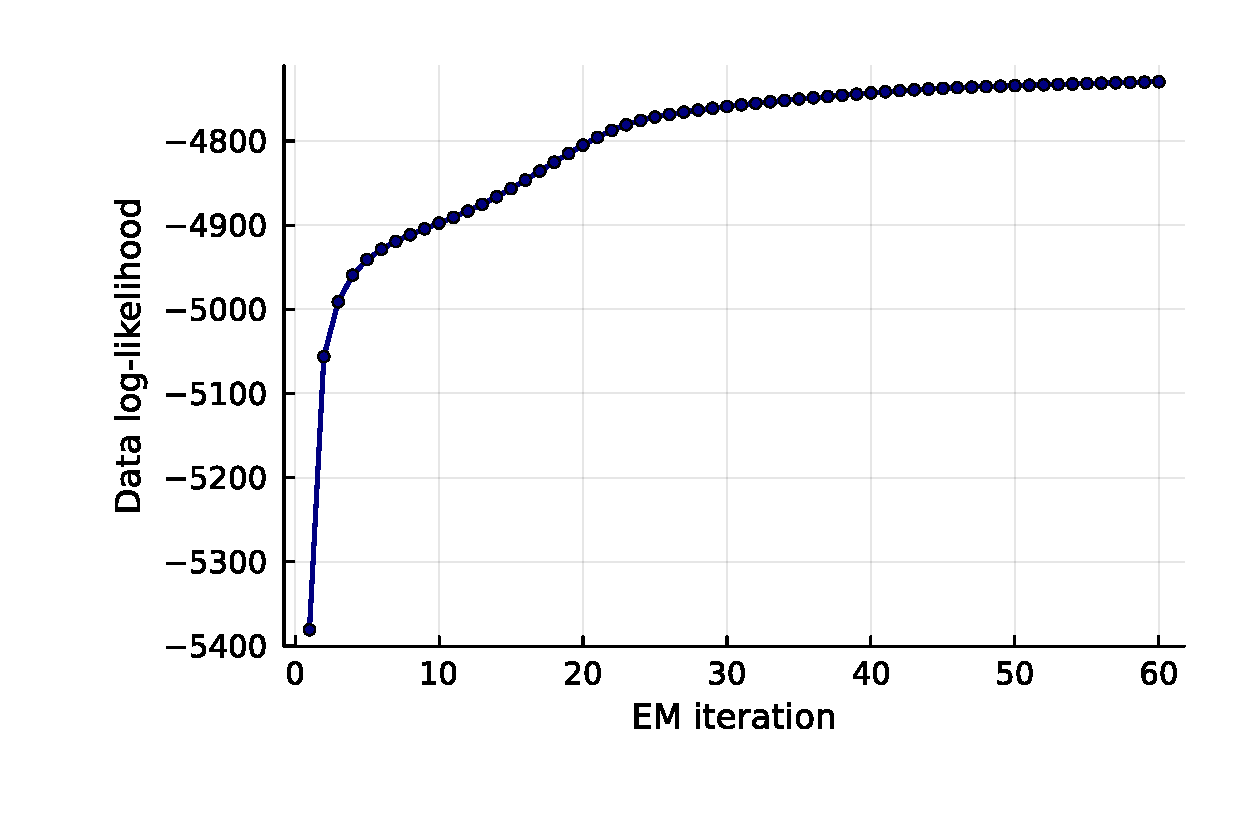
\includegraphics[width=\textwidth]{figs/Fig-Convergence-K18-t.pdf}
    \caption{CHMM-t}
\end{subfigure}
\hfill
\begin{subfigure}[b]{0.32\textwidth}
    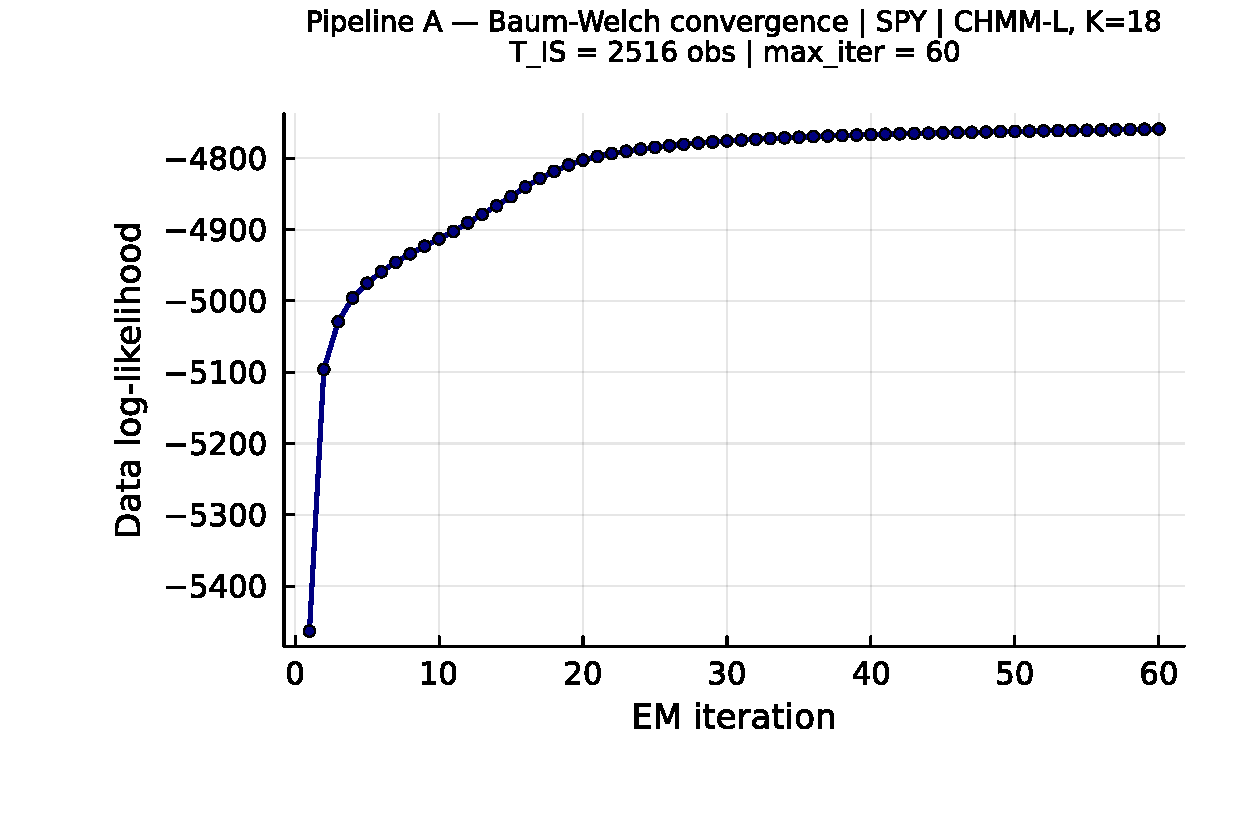
\includegraphics[width=\textwidth]{figs/Fig-Convergence-K18-L.pdf}
    \caption{CHMM-L}
\end{subfigure}
\caption{Log-likelihood histories for the SPY IS fit (Pipeline~A) at $K = 18$ across the three emission families (CHMM-N Gaussian classical EM; CHMM-t Student-t ECM with per-state $\nu_k$ golden-section sub-step; CHMM-L Laplace weighted-EM). All three curves are monotonically non-decreasing and plateau well before the $\texttt{max\_iter} = 60$ budget.}
\label{fig:convergence_families}
\end{figure}

\subsubsection{Ryd\'{e}n K = 2 Replication}
\label{sec:ryden_replication}

Table~\ref{tab:ryden_init} reports the direct replication of Ryd\'{e}n et al.'s 1998 $K = 2$ setting on SPY IS under both initialization strategies, as discussed in Section~\ref{sec:discussion}.
The quantile-based initialization used in the main body is row 1; five independent random-seed initializations are rows 2--6.
Random init here draws per-state $(\mu_k, \sigma_k)$ from a moderate perturbation of the sample moments, which is representative of the random-init practice common in the 1990s HMM literature.

\begin{table}[h]
\centering
\small
\caption{Ryd\'{e}n replication: $K = 2$ CHMM-N on SPY IS under quantile vs random initialization (seed sub-index varies the random init).}
\label{tab:ryden_init}
\begin{tabular}{l c c c c c}
\toprule
Init & KS IS (\%) & AD IS (\%) & ACF-MAE & Kurt IS & KS OoS (\%) \\
\midrule
Quantile (main body) & 79.0 & 71.5 & 0.0501 & 2.57 & 72.4 \\
Random seed = 1      & 78.7 & 70.7 & 0.0502 & 2.57 & 73.2 \\
Random seed = 7      & 75.3 & 69.6 & 0.0498 & 2.56 & 74.0 \\
Random seed = 42     & 77.6 & 70.0 & 0.0498 & 2.59 & 71.8 \\
Random seed = 100    & 76.2 & 69.4 & 0.0500 & 2.59 & 72.3 \\
Random seed = 2024   & 76.4 & 69.8 & 0.0499 & 2.54 & 72.9 \\
\bottomrule
\end{tabular}
\end{table}

The key observation is that ACF-MAE is essentially constant at $\approx 0.050$ across all six rows, matching the $K = 18$ CHMM-N of the main body.
IS KS pass rate remains below the $K = 18$ operating point ($75.3$--$79.0\%$) because two Gaussian components cannot tile the full multi-regime return distribution.
The combination is consistent with the reading that the binding low-$K$ constraint in the \citet{ryden1998stylized} setup is distributional rather than temporal: the ACF is already well reproduced at $K = 2$, and it is distributional fidelity that drives the preference for $K = 18$.



\subsection{Robustness, Test Power, Multi-Seed, and Auxiliary Baselines}
\label{sec:supp_robustness}
\subsection{OoS KS Test-Power Calibration}
\label{sec:ks_power}

Table~\ref{tab:ks_power} reports the two-sample KS test-power calibration used to anchor the OoS KS pass rates of Section~\ref{sec:oos}.
For each of $1{,}000$ Monte Carlo replications (seed = 20260420), a simulated series of length $T_{\text{OoS}} = 572$ is drawn from each of three reference generators and tested against the observed OoS series using the same $\alpha = 0.05$ threshold as the main-body pass-rate metric.

\begin{table}[h]
\centering
\small
\caption{OoS KS pass-rate calibration (1000 replications, seed = 20260420).}
\label{tab:ks_power}
\begin{tabular}{l c}
\toprule
Reference generator & Pass rate (\%) \\
\midrule
I.i.d.\ resamples of $R_{\text{OoS}}$ at length $T_{\text{OoS}} = 572$ (known-correct ceiling) & 100.0 \\
I.i.d.\ resamples of $R_{\text{IS}}$ at length $T_{\text{OoS}} = 572$ (nearly correct)          & 90.0  \\
Gaussian$(\hat\mu_{\text{IS}}, \hat\sigma_{\text{IS}})$ at length $T_{\text{IS}}$ (negative control) & 0.0 \\
\bottomrule
\end{tabular}
\end{table}

The $90.0\%$ "nearly correct" rate is the practical ceiling for the CHMM OoS KS pass rates reported in Section~\ref{sec:oos} ($80$--$84\%$); the $0\%$ rate on the Gaussian misspecified generator confirms that the KS test retains ample power at IS length to reject clearly wrong generators.

\subsection{Walk-Forward Rolling-Window Re-Estimation (Pipeline A)}
\label{sec:walk_forward}

This robustness check lives inside Pipeline A: the CHMM-N is still fit per ticker independently, only the fit window rolls forward. It does not introduce cross-asset coupling, and therefore should not be interpreted alongside the Pipeline B results in Section~\ref{sec:cross_asset}. Table~\ref{tab:walk_forward} reports the quarterly walk-forward re-estimation results referenced in Section~\ref{sec:cross_asset_univariate}.
The walk-forward protocol refits the CHMM-N every $63$ trading days (one quarter) across the $572$-day OoS window, feeding the realized returns of the prior quarter into the training set before each refit.
The rolling protocol recovers a modest $\sim 1$ percentage point on JNJ and a substantial $\sim 15$ percentage points on JPM relative to the fixed-IS baseline, confirming that the stationarity assumption is the principal contributor to the JPM OoS gap while JNJ's OoS gap is already small under the fixed fit.

\begin{table}[h]
\centering
\small
\caption{\textbf{Walk-forward (quarterly CHMM-N refit) vs fixed-IS CHMM-N on JNJ and JPM} (Pipeline A, per-ticker independent fits; walk-forward only rolls the fit window, it does not introduce cross-asset dependence). $K = 18$, 1000 simulated paths per (ticker, mode), seed = 20260420. IS window 2014-01-03 through 2024-01-03; OoS window 2024-01-04 through 2026-04-17 ($T_{\text{OoS}} = 572$). The walk-forward mode refits the CHMM-N every 63 trading days across the OoS window, feeding each completed quarter's realized returns back into the training set before the next refit. Columns report percent KS / AD pass rate at $\alpha = 0.05$, excess kurtosis, ACF-MAE of $|G_t|$, Wasserstein-1, and Hellinger distance.}
\label{tab:walk_forward}
\resizebox{\textwidth}{!}{%
\begin{tabular}{l cc cc cc c c c}
\toprule
Mode & KS IS & AD IS & KS OoS & AD OoS & Kurt IS & Kurt OoS & ACF-MAE & $W_1$ & $H$ \\
\midrule
JNJ fixed-IS      & 99.3 & 98.2 & 94.0 & 92.1 & 5.46 & 4.98 & 0.0322 & 0.095 & 0.0786 \\
JNJ walk-forward  & 99.3 & 98.2 & 94.9 & 91.3 & 5.46 & 5.14 & 0.0322 & 0.095 & 0.0786 \\
JPM fixed-IS      & 96.6 & 94.4 & 49.0 & 48.6 & 7.33 & 6.31 & 0.0449 & 0.165 & 0.0875 \\
JPM walk-forward  & 96.6 & 94.4 & 64.3 & 63.6 & 7.33 & 5.96 & 0.0449 & 0.165 & 0.0875 \\
\bottomrule
\end{tabular}%
}
\end{table}

\subsection{Block-Bootstrap Baseline}
\label{sec:block_bootstrap_supp}

Table~\ref{tab:block_bootstrap} reports the full seven-metric panel for the stationary block bootstrap at block length $b = 10$ trading days, the temporally-aware non-parametric baseline added to Table~\ref{tab:model_comparison}.

\begin{table}[h]
\centering
\small
\caption{Stationary block bootstrap (block length $b = 10$ trading days) on SPY (1000 paths, seed = 20260420).}
\label{tab:block_bootstrap}
\begin{tabular}{l cc cc c c c c}
\toprule
Window & KS & AD & Kurt & ACF-MAE & $W_1$ & $H$ & Cov \\
\midrule
IS  & 99.2 & 96.4 & 7.07 & 0.0568 & 0.092 & 0.0534 & 100.0 \\
OoS & 87.5 & 86.4 & 5.34 & 0.0512 & 0.225 & 0.1570 & 86.9  \\
\bottomrule
\end{tabular}
\end{table}

\subsection{Discrete HMM with Bin-Conditional Student-t Emissions}
\label{sec:bin_t_supp}

Table~\ref{tab:bin_t} reports the full seven-metric panel for the Bin-T NJ variant referenced in Section~\ref{sec:model_comparison}: the discrete NJ transition matrix with $K_{\text{disc}} = 13$ quantile bins, but with each bin emitting from a bin-conditional Student-t density rather than from the bin centroid.

\begin{table}[h]
\centering
\small
\caption{Discrete HMM with bin-conditional Student-t emissions on SPY (no jumps, $K_{\text{disc}} = 13$, 1000 paths, seed = 20260420).}
\label{tab:bin_t}
\begin{tabular}{l cc cc c c c c}
\toprule
Window & KS & AD & Kurt & ACF-MAE & $W_1$ & $H$ & Cov \\
\midrule
IS  & 95.4 & 92.1 & 26.18 & 0.0619 & 0.116 & 0.0929 & 89.9 \\
OoS & 86.7 & 93.2 & 10.76 & 0.0538 & 0.177 & 0.1614 & 93.9 \\
\bottomrule
\end{tabular}
\end{table}

The bin-conditional Student-t fit picks $\nu \approx 2.71$ for the two extreme bins (bins $1$ and $13$, corresponding to the lower and upper quantile tails of the IS distribution) and $\nu = 50$ (upper bracket) for the eleven central bins, which explains both the large in-sample simulated kurtosis ($26.18$) and the very thin-scale central bins ($\sigma$ $\sim$ $0.06$--$0.28$).



\subsection{GRU Deep-Generative Baseline}
\label{sec:gru_supp}

Architecture and training details for the GRU baseline used in
Section~\ref{sec:model_comparison} are summarised here.

\begin{itemize}
    \item \textbf{Architecture.} A single-layer Gated Recurrent Unit (GRU)
    with hidden dimension $H = 32$ followed by a Dense head with two
    outputs $(\mu_t, \log \sigma_t)$. Input is a single feature (the
    standardised return) over a context window of $w = 20$ trading days.

    \item \textbf{Loss.} Per-window negative log-likelihood of a Gaussian
    next-step density, equation~\eqref{eq:gru_nll}.

    \item \textbf{Optimiser.} Adam, learning rate $1.0 \times 10^{-3}$.

    \item \textbf{Training schedule.} $20$ epochs, full pass per epoch
    over $T_{\text{IS}} - w$ training windows, randomly shuffled at each
    epoch.

    \item \textbf{Numerical stability.} $\log \sigma_t$ is clamped to
    $[-6, 4]$ inside the loss to prevent gradient explosion when the
    network attempts to assign vanishingly-small variance to extreme
    observations.

    \item \textbf{Pre-processing.} The input return series is standardised
    by its in-sample mean and standard deviation; predictions are
    re-scaled back at sampling time.

    \item \textbf{Synthesis.} The trailing $w$ in-sample returns seed the
    recurrence; for each generation step the predicted Gaussian is
    sampled, the sample is appended to the context window, and the
    procedure rolls forward. The first $64$ steps are discarded as
    burn-in.

    \item \textbf{Implementation.} Julia using \texttt{Flux.jl}
    \cite{innes2018flux} with the \texttt{Optimisers.Adam} state.
    Random seed for weight initialisation, training shuffling, and per-path
    sampling: $20260420$, with deterministic per-path sub-seeds.
\end{itemize}

The trained model is callable through the same
\texttt{simulate\_gru(model, n\_steps; seed\_window)} interface as the
CHMM and discrete-HMM models, so the seven-metric panel evaluates the GRU
on byte-identical windows to the other generators.

\begin{table}[h]
\centering
\small
\caption{GRU deep-generative baseline on SPY (single-layer, hidden $H=32$, window $w=20$, $20$ epochs, Adam $\eta=10^{-3}$, $1{,}000$ paths, seed = 20260420). Final training NLL: $0.2005$.}
\label{tab:gru}
\begin{tabular}{l cc c c c c c}
\toprule
Window & KS & AD & Kurt & ACF-MAE & $W_1$ & $H$ & Cov \\
\midrule
IS  & 18.1 & 13.7 & 2.85 & 0.0518 & 0.196 & 0.0966 & 37.4 \\
OoS & 52.5 & 55.0 & 2.21 & 0.0500 & 0.293 & 0.1603 & 69.7 \\
\bottomrule
\end{tabular}
\end{table}

\subsection{Per-Ticker OoS Price-Simulation Figures (Unconditional CHMM)}
\label{sec:price_sim_oos_appendix}

This appendix collects the per-ticker price-fan and terminal-distribution figures deferred from Section~\ref{sec:price_sim_oos} for the four non-body tickers JNJ, JPM, AAPL, and QQQ.
All figures use the same plotting conventions as Figure~\ref{fig:price_fan_spy} in the main body: blue shaded bands are the $5$--$95\%$ and $25$--$75\%$ quantile envelopes of the $500$ simulated paths, blue solid line is the simulated median, red solid line is the observed OoS price track.
Terminal histograms follow the conventions of Figure~\ref{fig:price_terminal_hists}.
Summary metrics for all four tickers are in Tables~\ref{tab:price_sim_oos} and~\ref{tab:price_sim_path_metrics} in the main body.

\begin{figure}[h]
\centering
\begin{subfigure}[t]{0.32\textwidth}
    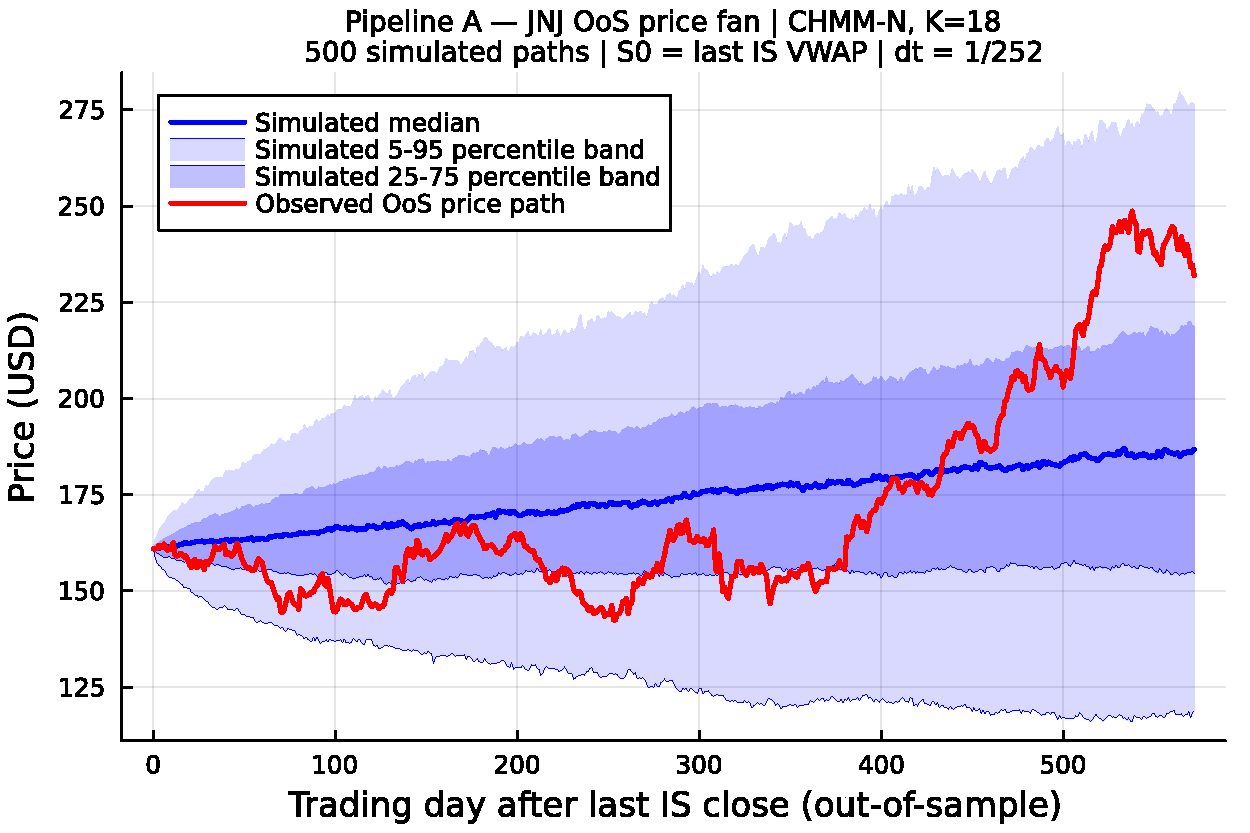
\includegraphics[width=\textwidth]{figs/Fig-JNJ-PriceFan-N.pdf}
    \caption{CHMM-N.}
\end{subfigure}
\begin{subfigure}[t]{0.32\textwidth}
    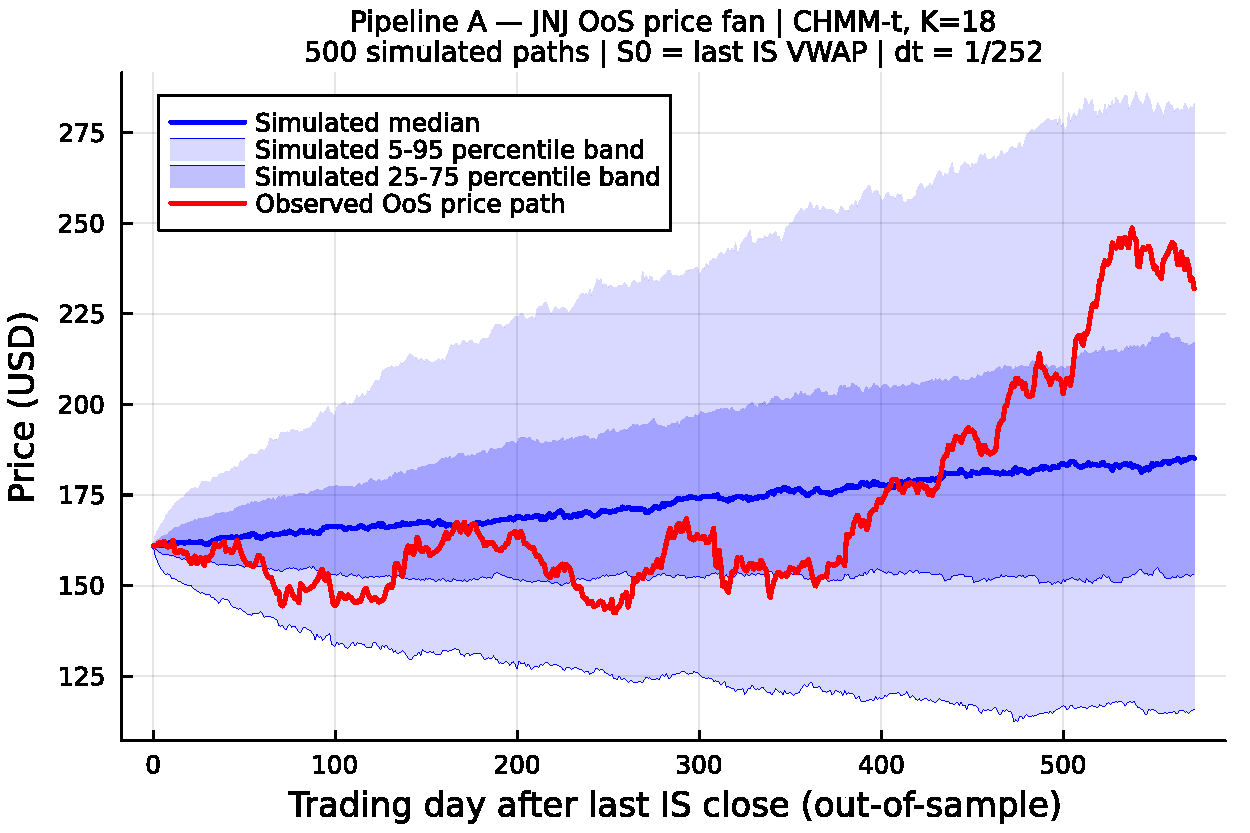
\includegraphics[width=\textwidth]{figs/Fig-JNJ-PriceFan-t.pdf}
    \caption{CHMM-t.}
\end{subfigure}
\begin{subfigure}[t]{0.32\textwidth}
    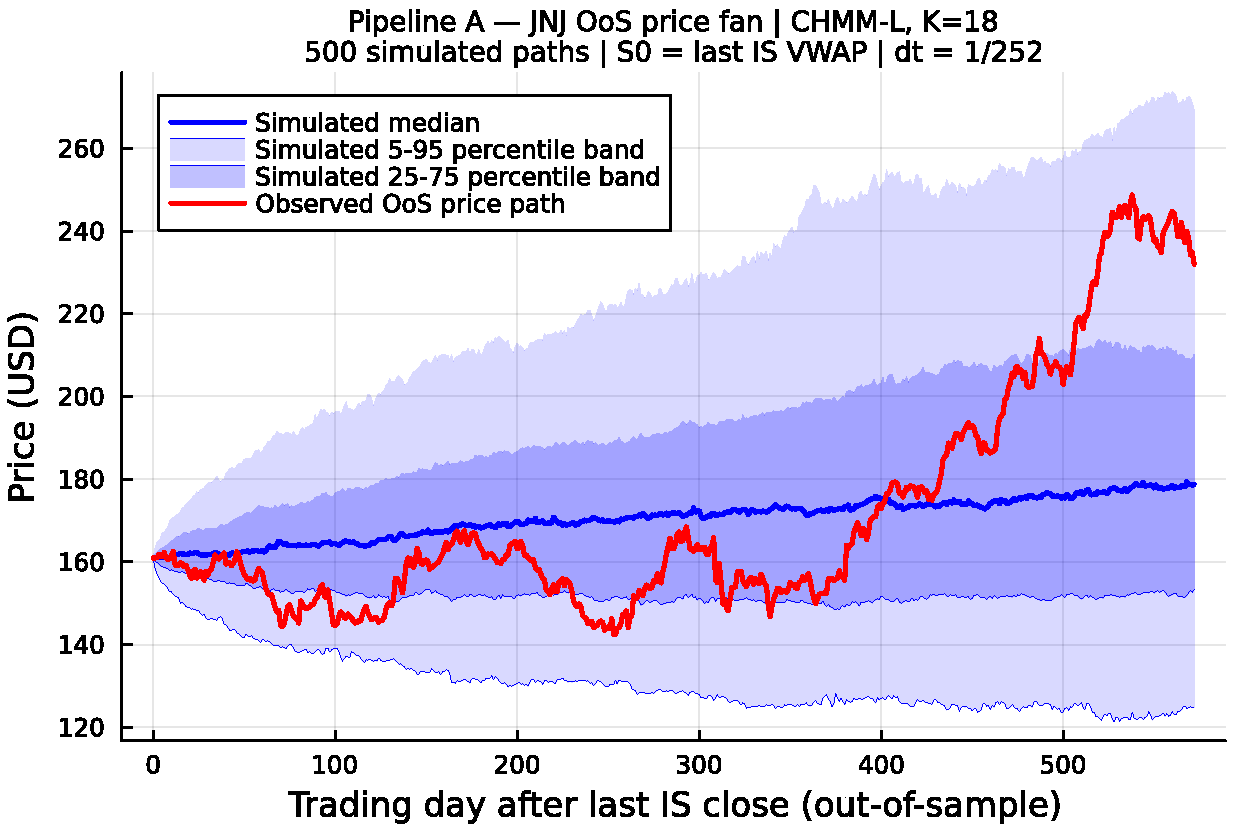
\includegraphics[width=\textwidth]{figs/Fig-JNJ-PriceFan-L.pdf}
    \caption{CHMM-L.}
\end{subfigure}
\caption{JNJ out-of-sample price fan, unconditional CHMM sampler.}
\label{fig:price_fan_jnj_appendix}
\end{figure}

\begin{figure}[h]
\centering
\begin{subfigure}[t]{0.32\textwidth}
    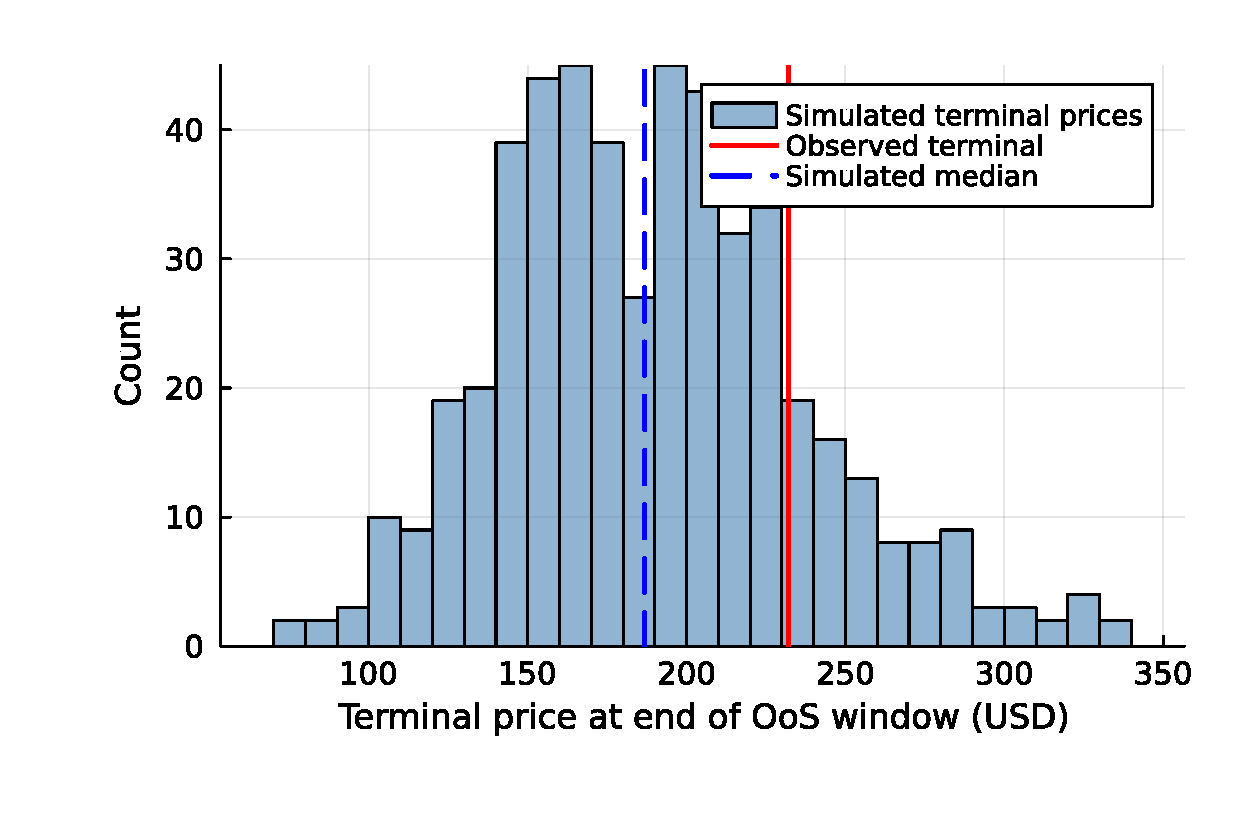
\includegraphics[width=\textwidth]{figs/Fig-JNJ-TerminalDist-N.pdf}
    \caption{CHMM-N.}
\end{subfigure}
\begin{subfigure}[t]{0.32\textwidth}
    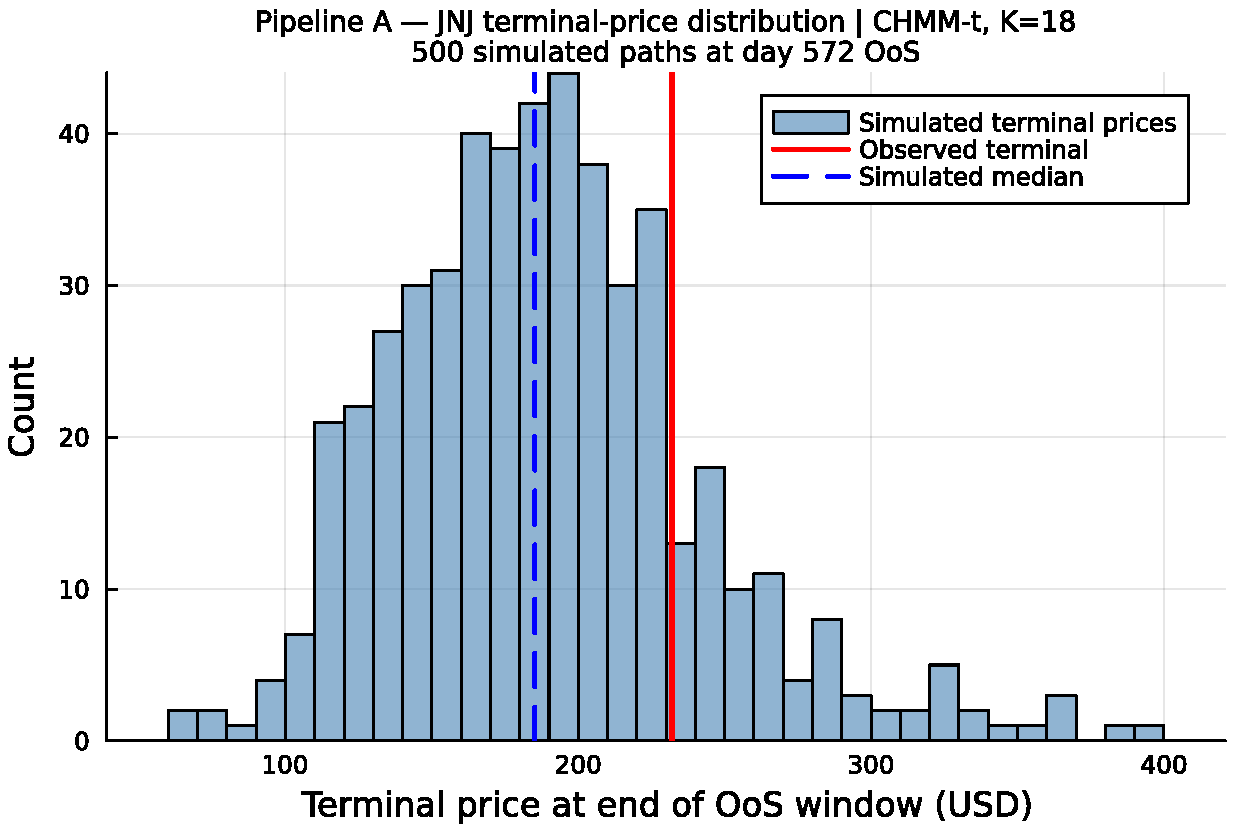
\includegraphics[width=\textwidth]{figs/Fig-JNJ-TerminalDist-t.pdf}
    \caption{CHMM-t.}
\end{subfigure}
\begin{subfigure}[t]{0.32\textwidth}
    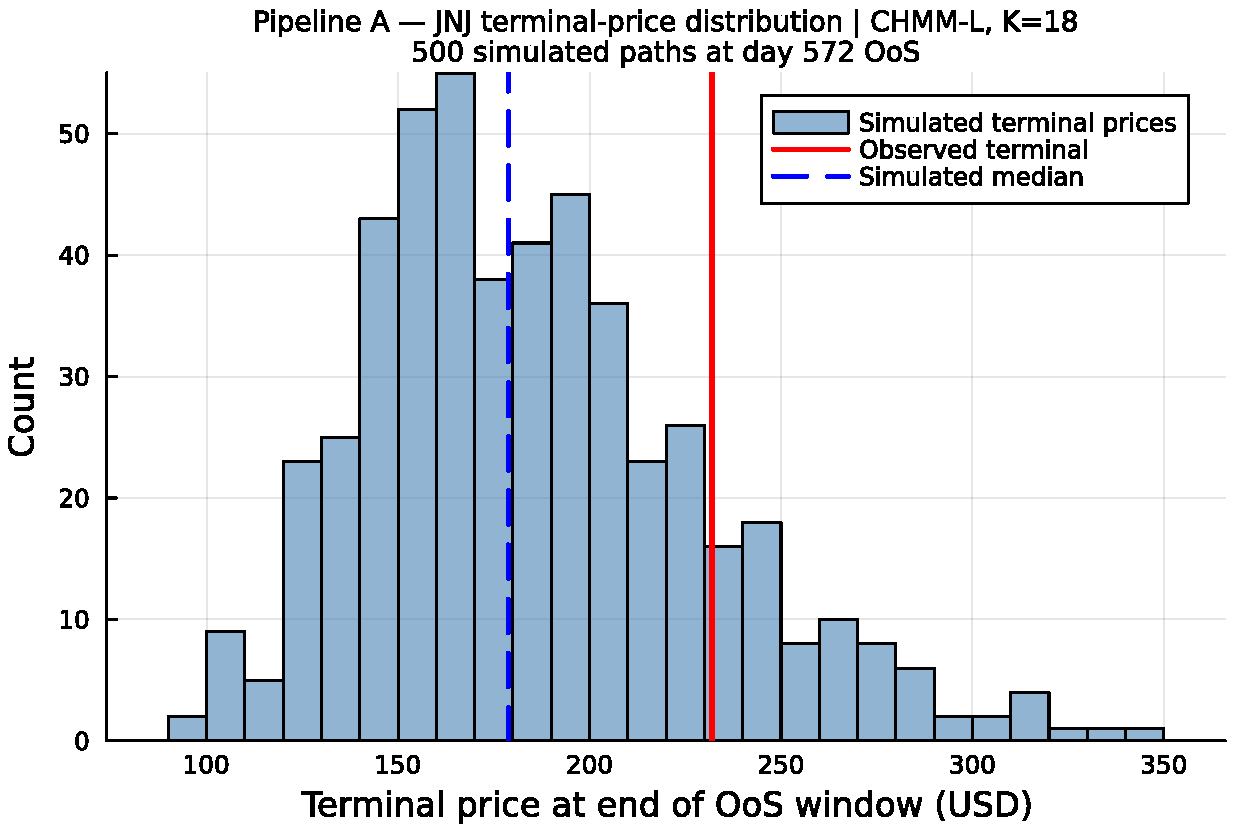
\includegraphics[width=\textwidth]{figs/Fig-JNJ-TerminalDist-L.pdf}
    \caption{CHMM-L.}
\end{subfigure}
\caption{JNJ terminal-price distribution, unconditional CHMM sampler.}
\label{fig:terminal_jnj_appendix}
\end{figure}

\begin{figure}[h]
\centering
\begin{subfigure}[t]{0.32\textwidth}
    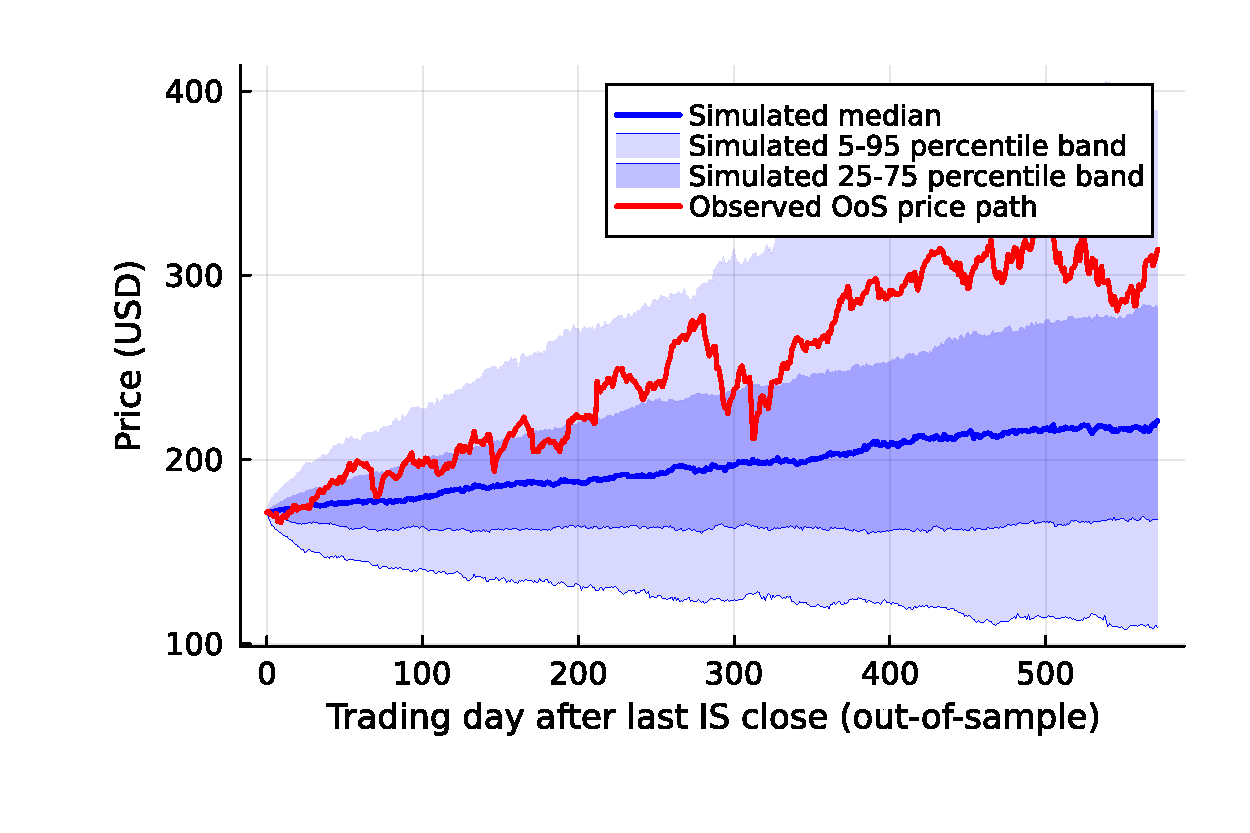
\includegraphics[width=\textwidth]{figs/Fig-JPM-PriceFan-N.pdf}
    \caption{CHMM-N.}
\end{subfigure}
\begin{subfigure}[t]{0.32\textwidth}
    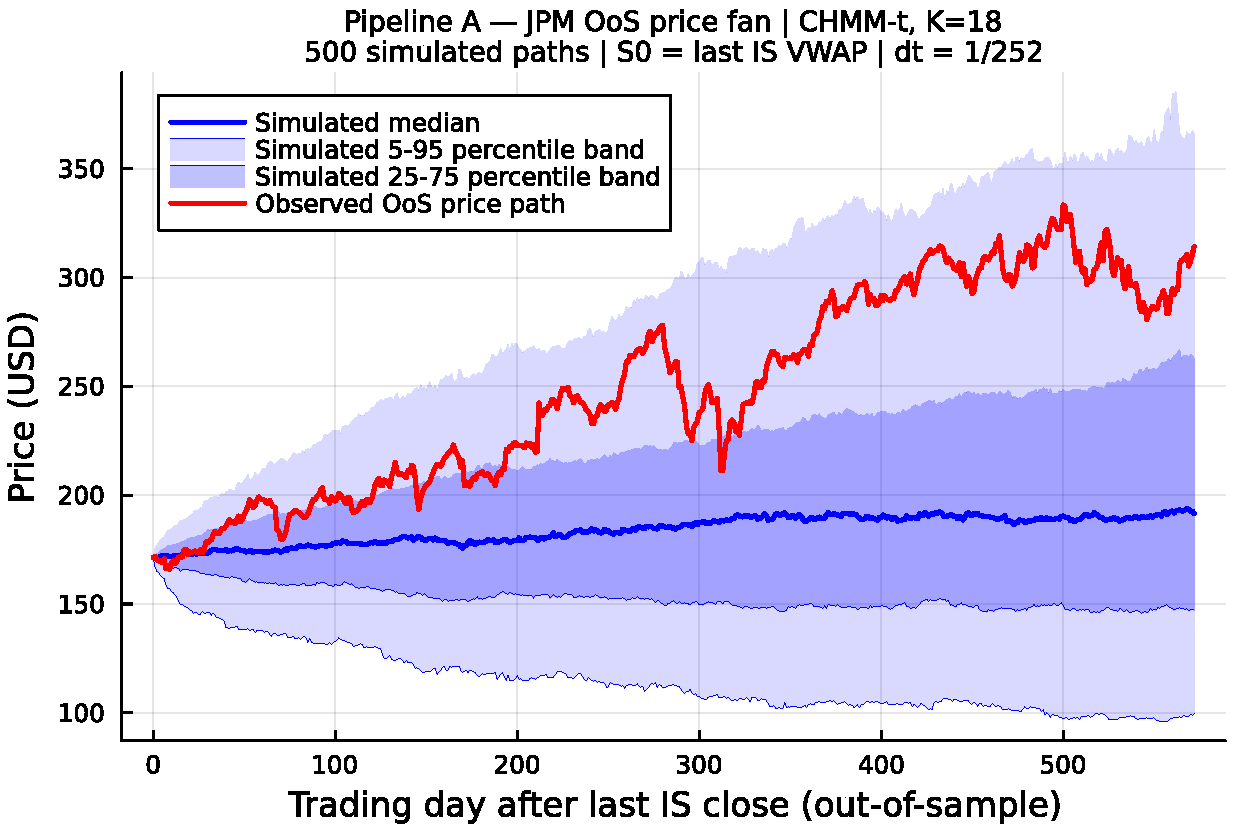
\includegraphics[width=\textwidth]{figs/Fig-JPM-PriceFan-t.pdf}
    \caption{CHMM-t.}
\end{subfigure}
\begin{subfigure}[t]{0.32\textwidth}
    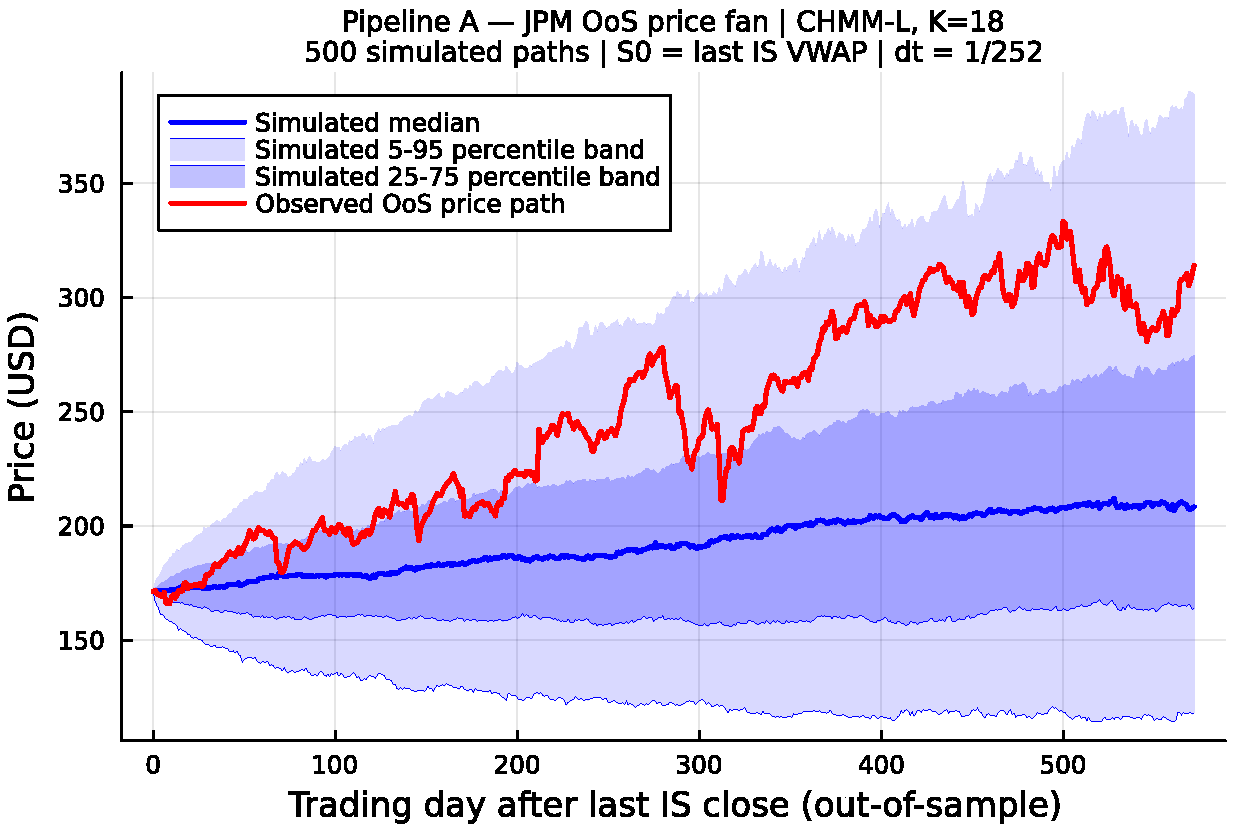
\includegraphics[width=\textwidth]{figs/Fig-JPM-PriceFan-L.pdf}
    \caption{CHMM-L.}
\end{subfigure}
\caption{JPM out-of-sample price fan, unconditional CHMM sampler.}
\label{fig:price_fan_jpm_appendix}
\end{figure}

\begin{figure}[h]
\centering
\begin{subfigure}[t]{0.32\textwidth}
    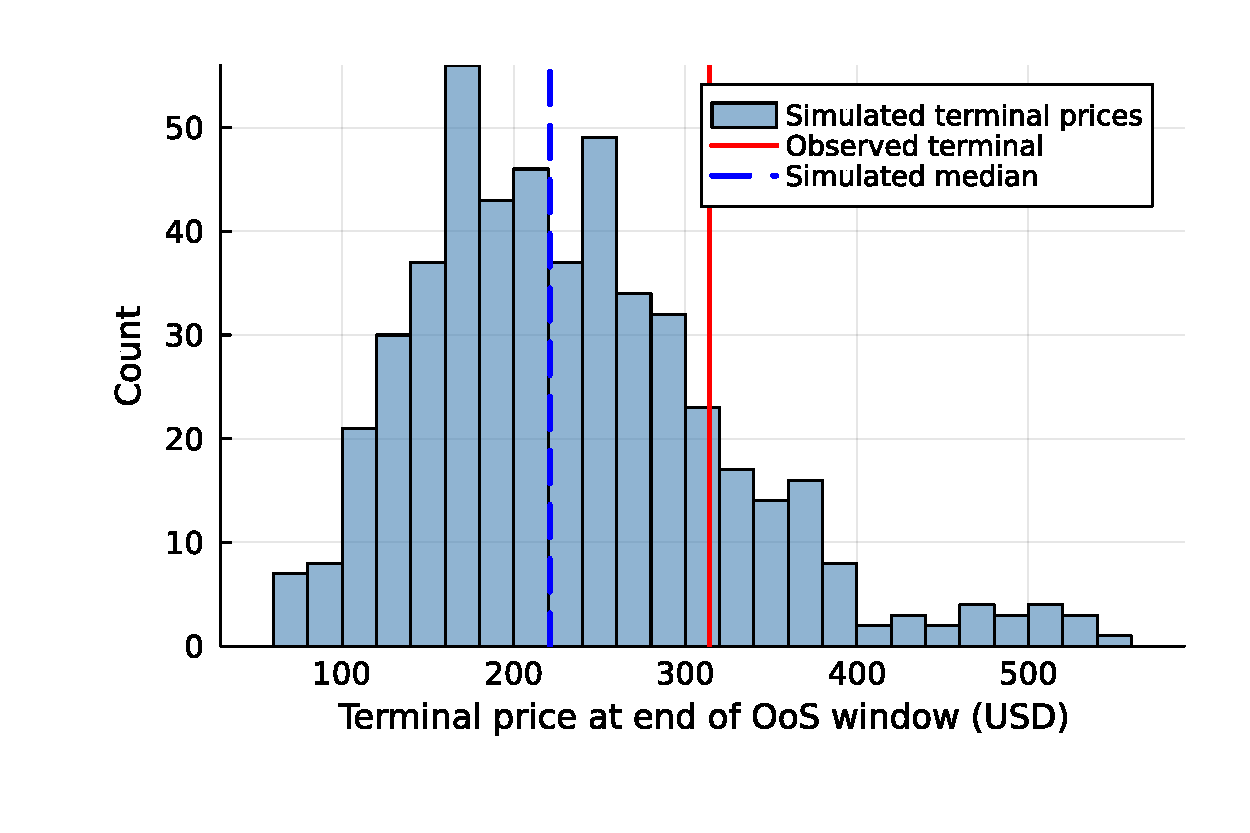
\includegraphics[width=\textwidth]{figs/Fig-JPM-TerminalDist-N.pdf}
    \caption{CHMM-N.}
\end{subfigure}
\begin{subfigure}[t]{0.32\textwidth}
    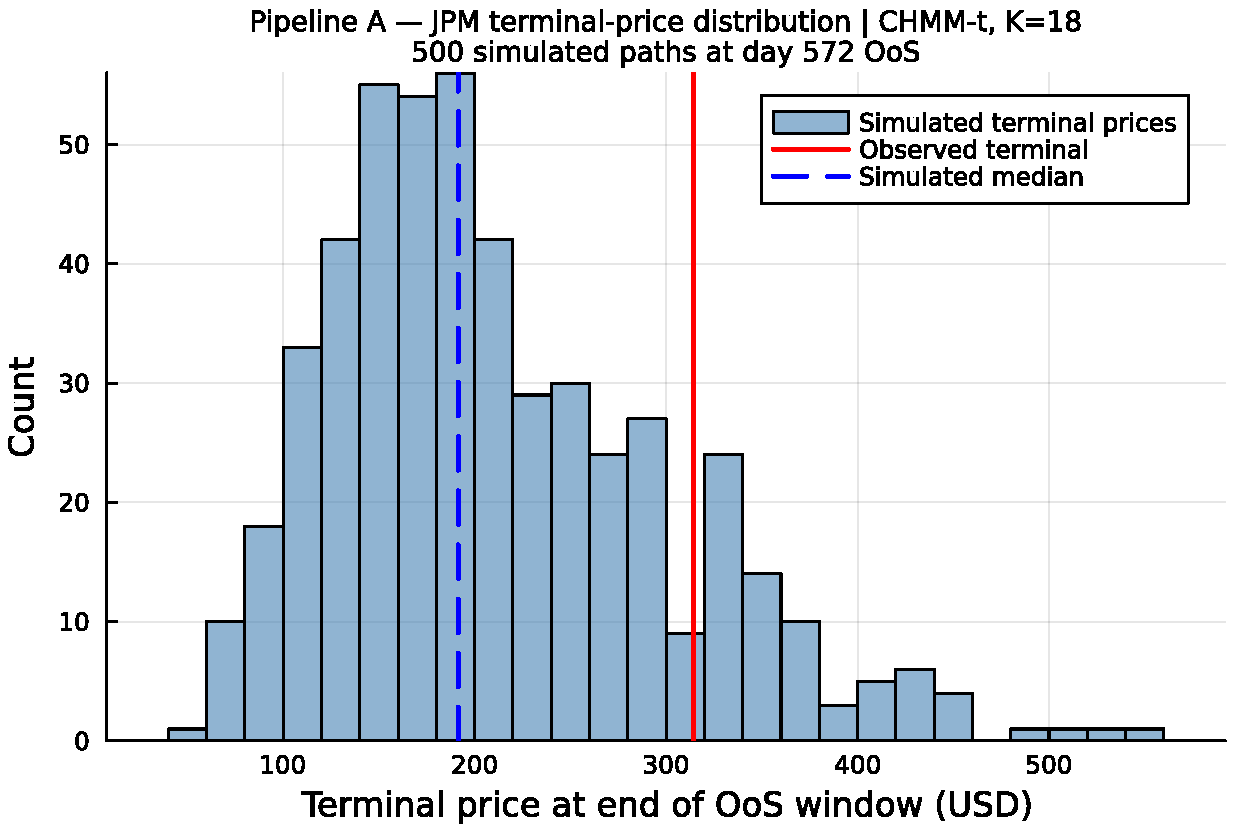
\includegraphics[width=\textwidth]{figs/Fig-JPM-TerminalDist-t.pdf}
    \caption{CHMM-t.}
\end{subfigure}
\begin{subfigure}[t]{0.32\textwidth}
    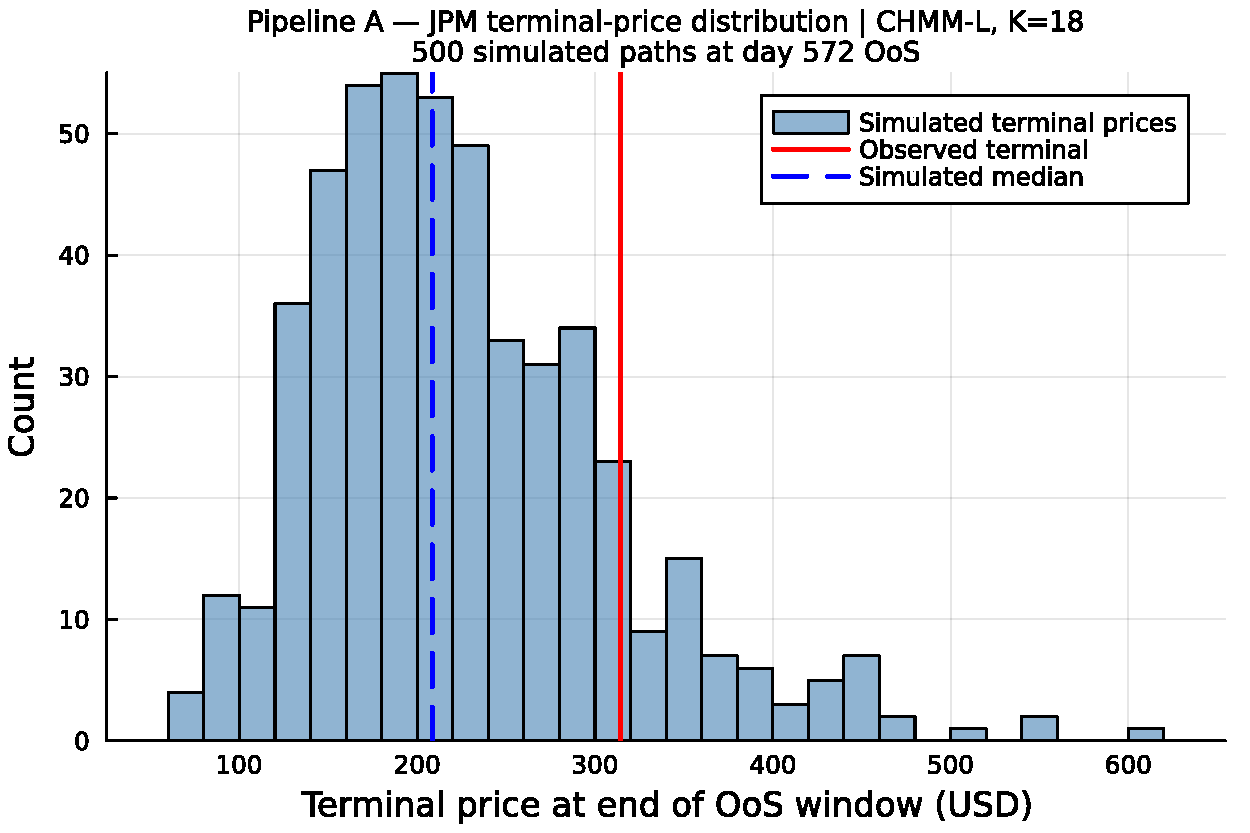
\includegraphics[width=\textwidth]{figs/Fig-JPM-TerminalDist-L.pdf}
    \caption{CHMM-L.}
\end{subfigure}
\caption{JPM terminal-price distribution, unconditional CHMM sampler.}
\label{fig:terminal_jpm_appendix}
\end{figure}

\begin{figure}[h]
\centering
\begin{subfigure}[t]{0.32\textwidth}
    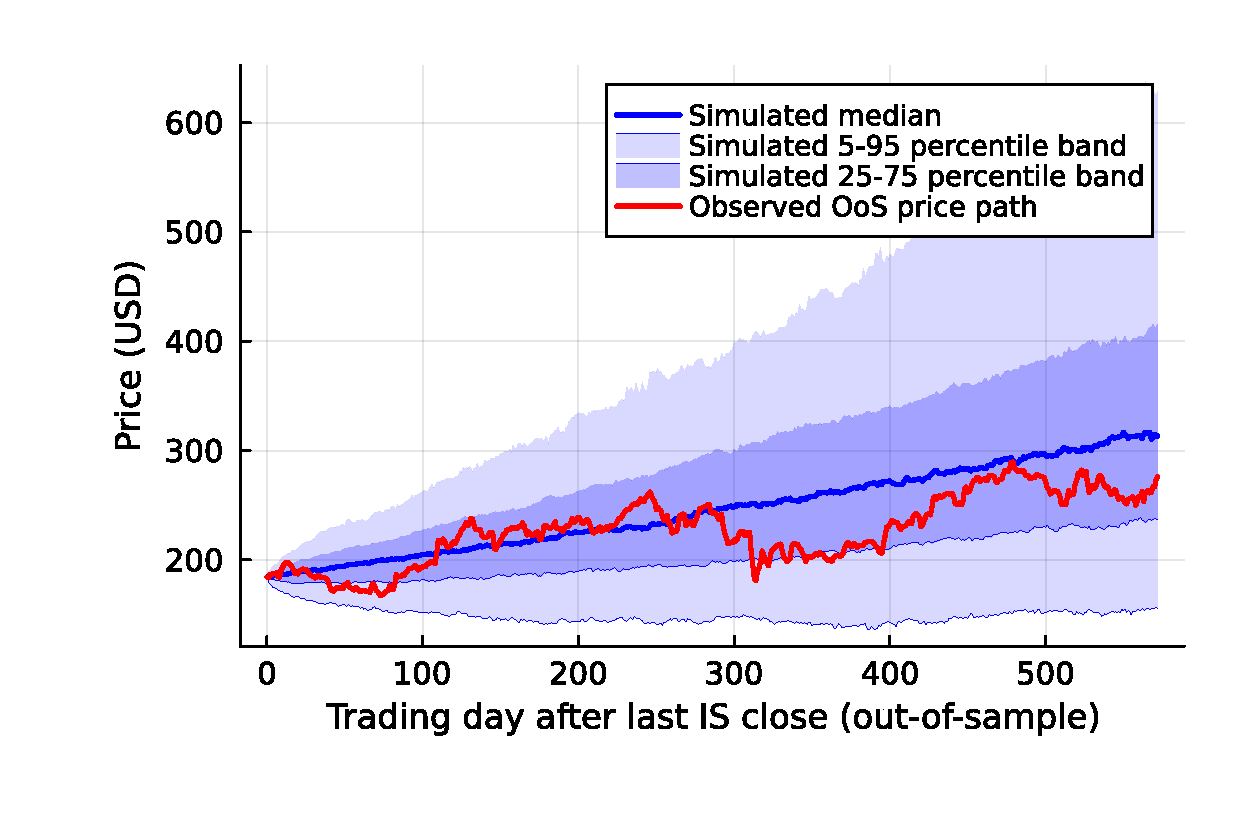
\includegraphics[width=\textwidth]{figs/Fig-AAPL-PriceFan-N.pdf}
    \caption{CHMM-N.}
\end{subfigure}
\begin{subfigure}[t]{0.32\textwidth}
    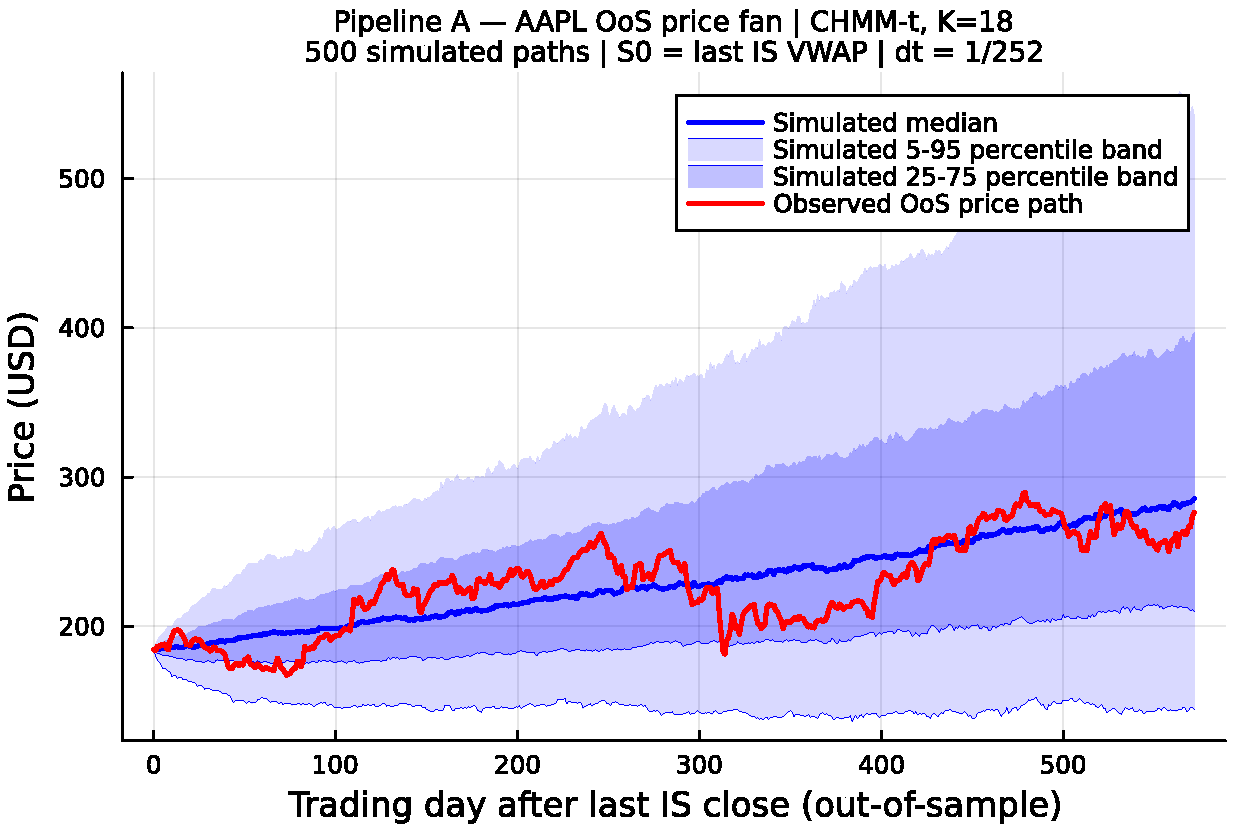
\includegraphics[width=\textwidth]{figs/Fig-AAPL-PriceFan-t.pdf}
    \caption{CHMM-t.}
\end{subfigure}
\begin{subfigure}[t]{0.32\textwidth}
    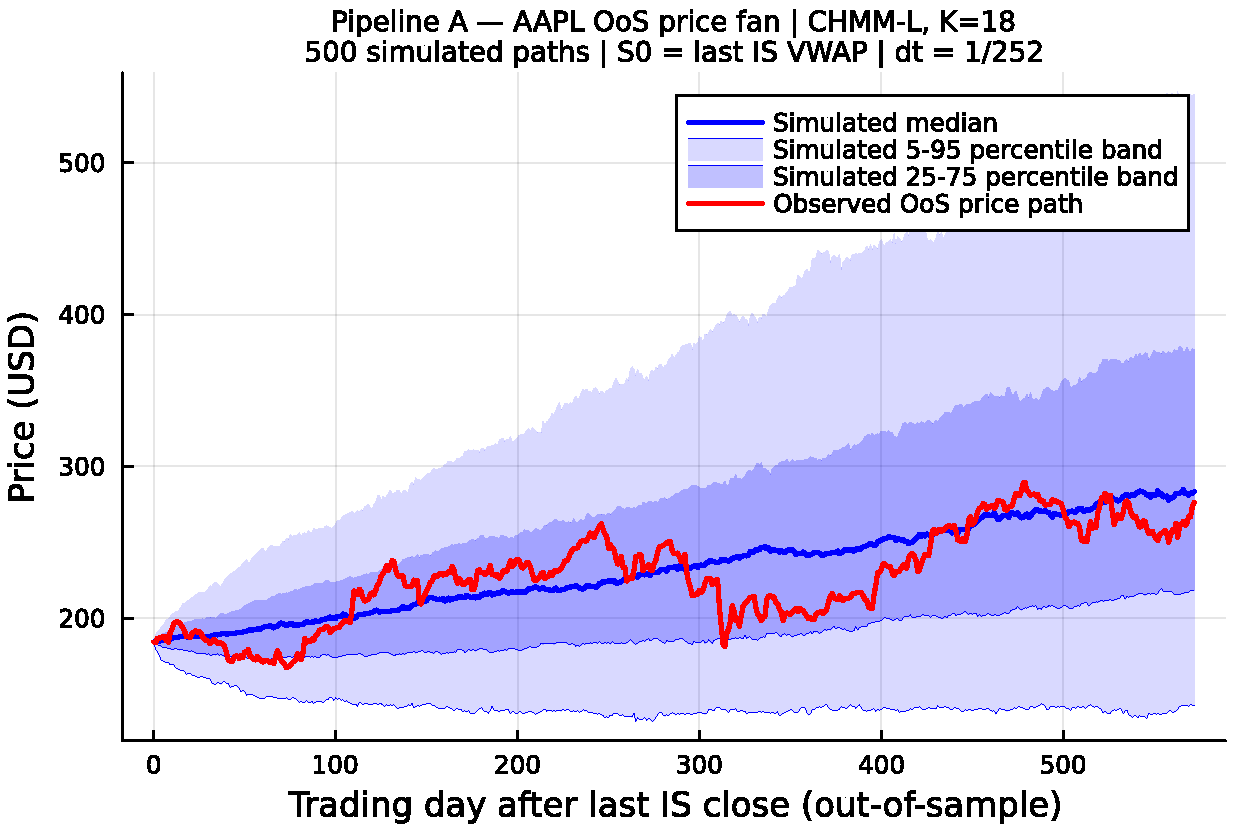
\includegraphics[width=\textwidth]{figs/Fig-AAPL-PriceFan-L.pdf}
    \caption{CHMM-L.}
\end{subfigure}
\caption{AAPL out-of-sample price fan, unconditional CHMM sampler.}
\label{fig:price_fan_aapl_appendix}
\end{figure}

\begin{figure}[h]
\centering
\begin{subfigure}[t]{0.32\textwidth}
    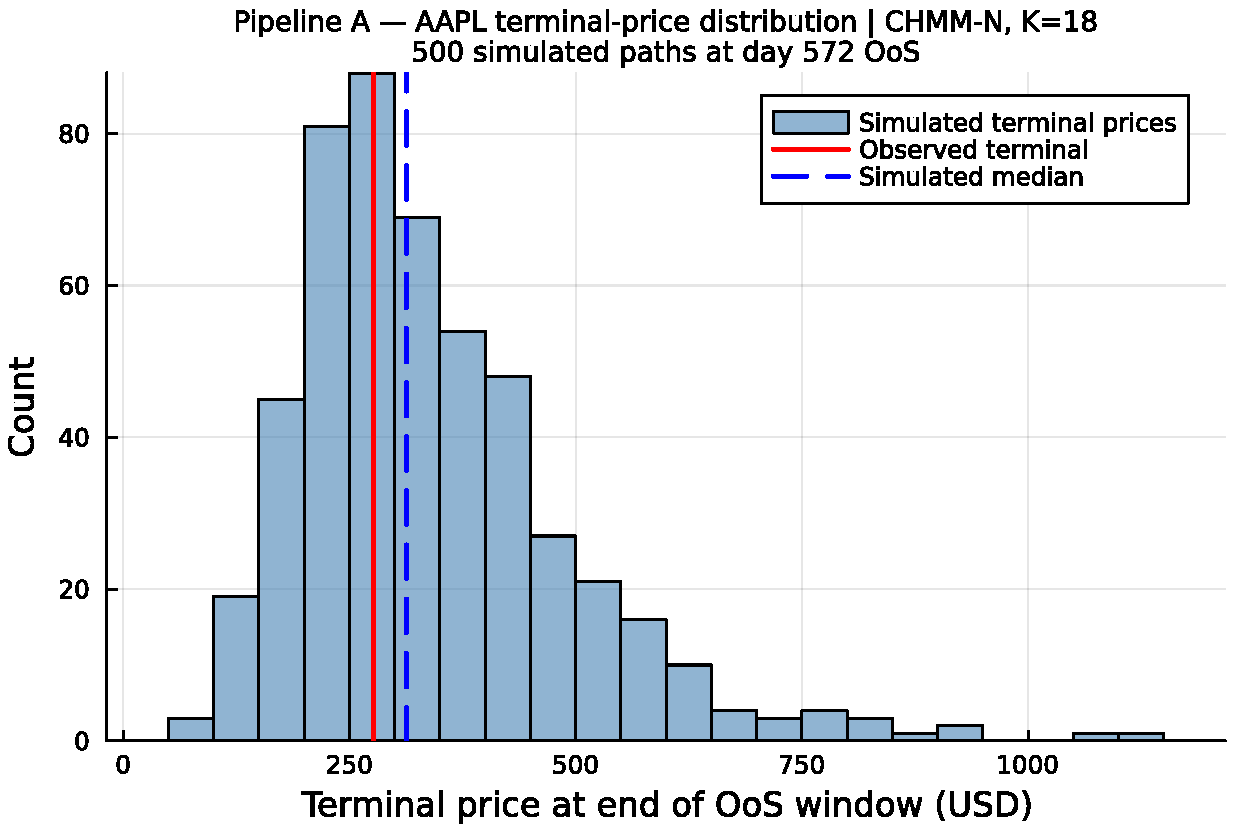
\includegraphics[width=\textwidth]{figs/Fig-AAPL-TerminalDist-N.pdf}
    \caption{CHMM-N.}
\end{subfigure}
\begin{subfigure}[t]{0.32\textwidth}
    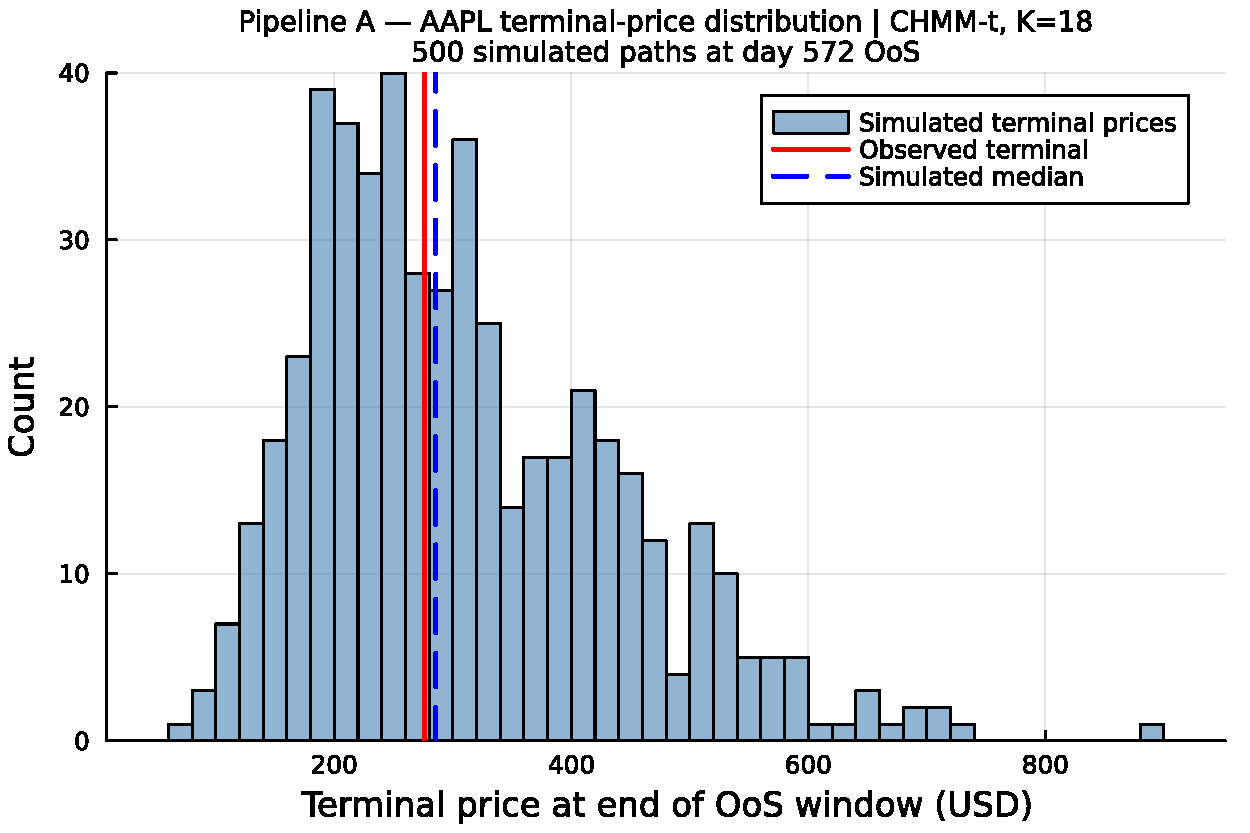
\includegraphics[width=\textwidth]{figs/Fig-AAPL-TerminalDist-t.pdf}
    \caption{CHMM-t.}
\end{subfigure}
\begin{subfigure}[t]{0.32\textwidth}
    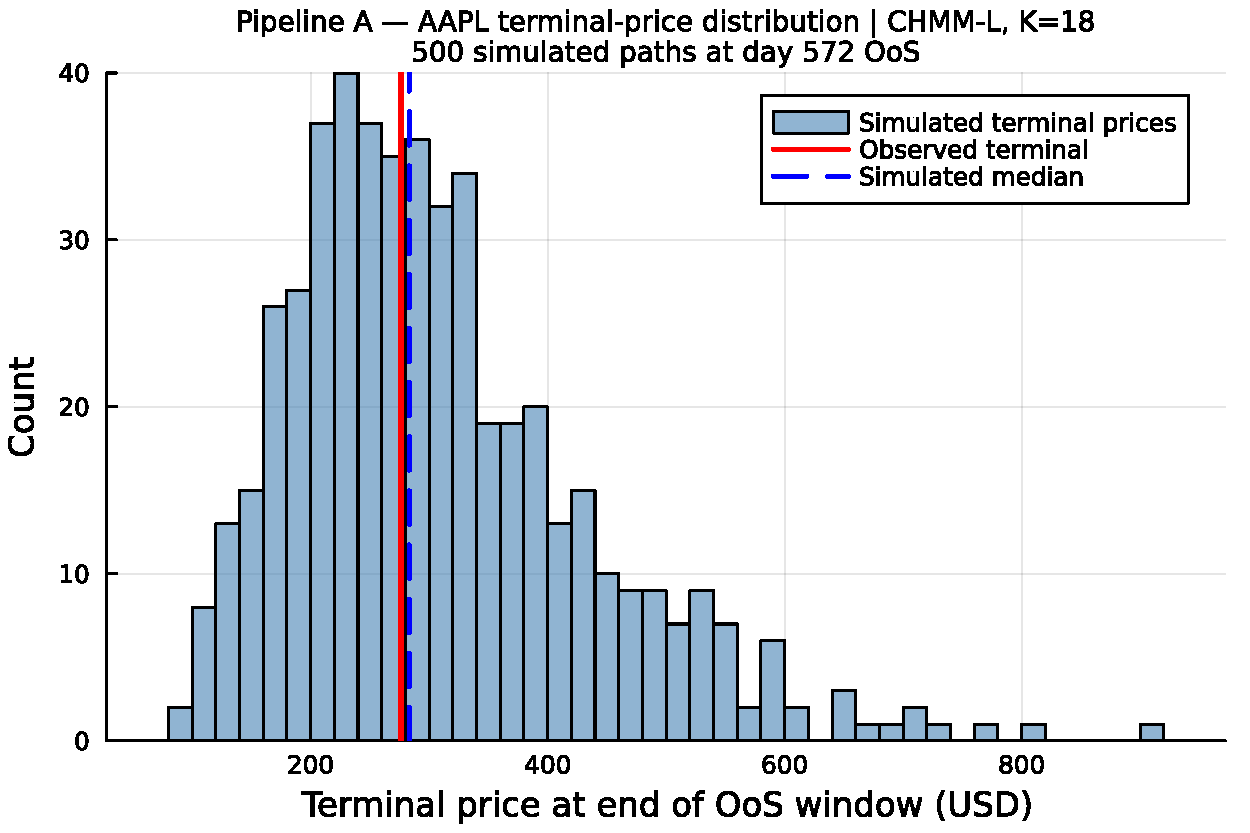
\includegraphics[width=\textwidth]{figs/Fig-AAPL-TerminalDist-L.pdf}
    \caption{CHMM-L.}
\end{subfigure}
\caption{AAPL terminal-price distribution, unconditional CHMM sampler.}
\label{fig:terminal_aapl_appendix}
\end{figure}

\begin{figure}[h]
\centering
\begin{subfigure}[t]{0.32\textwidth}
    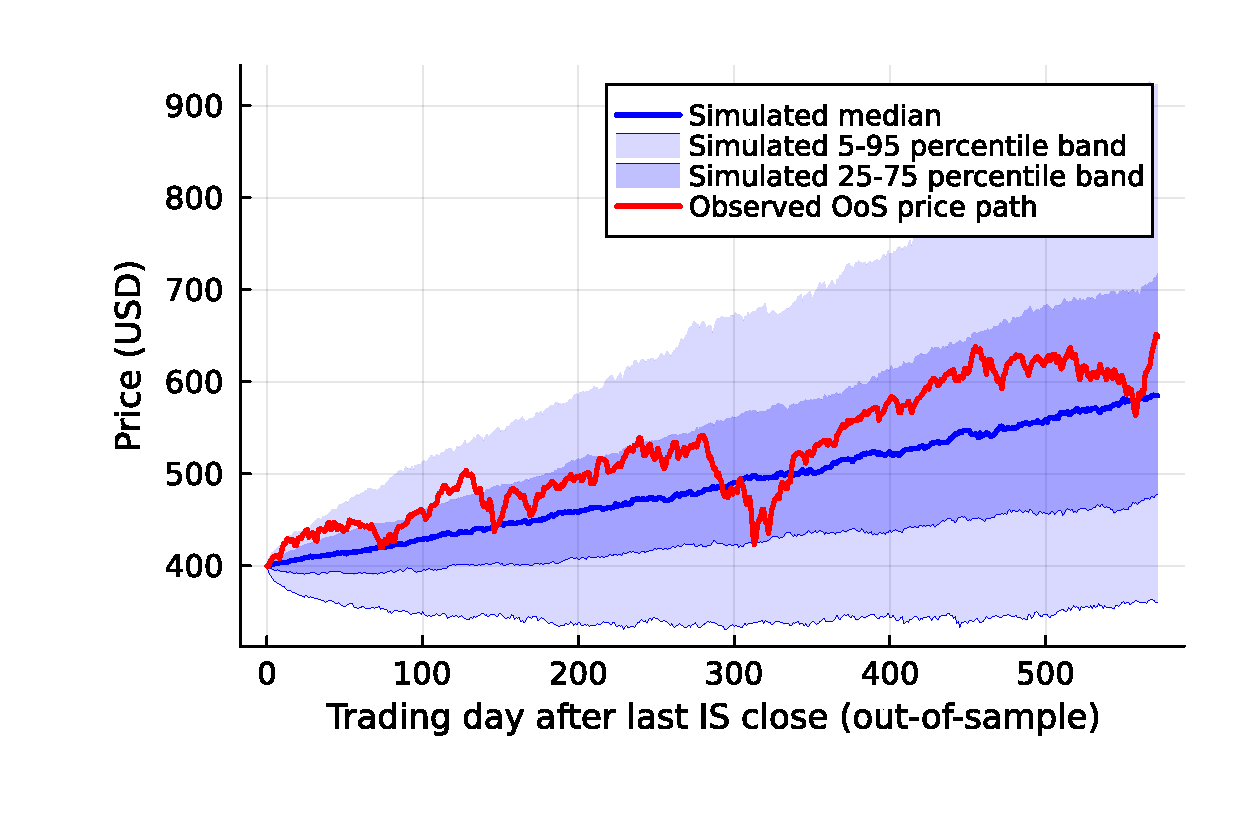
\includegraphics[width=\textwidth]{figs/Fig-QQQ-PriceFan-N.pdf}
    \caption{CHMM-N.}
\end{subfigure}
\begin{subfigure}[t]{0.32\textwidth}
    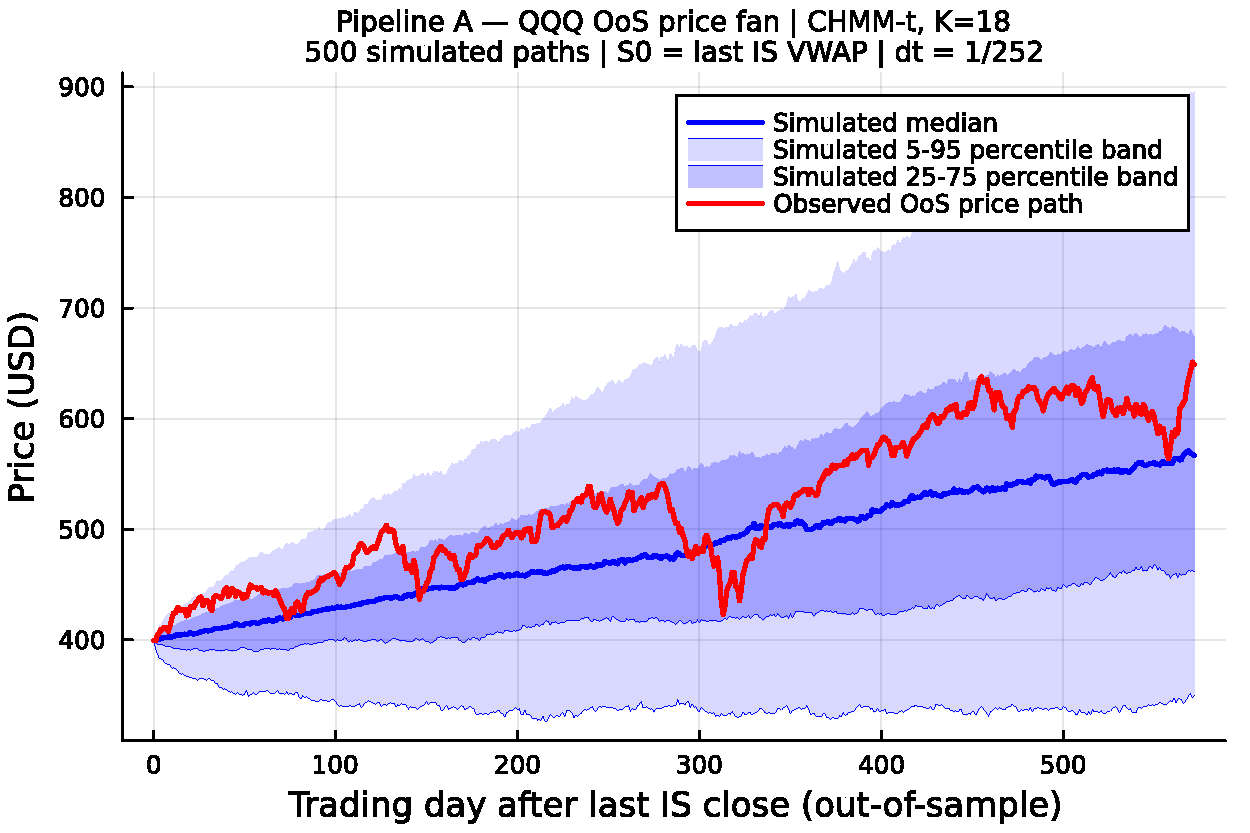
\includegraphics[width=\textwidth]{figs/Fig-QQQ-PriceFan-t.pdf}
    \caption{CHMM-t.}
\end{subfigure}
\begin{subfigure}[t]{0.32\textwidth}
    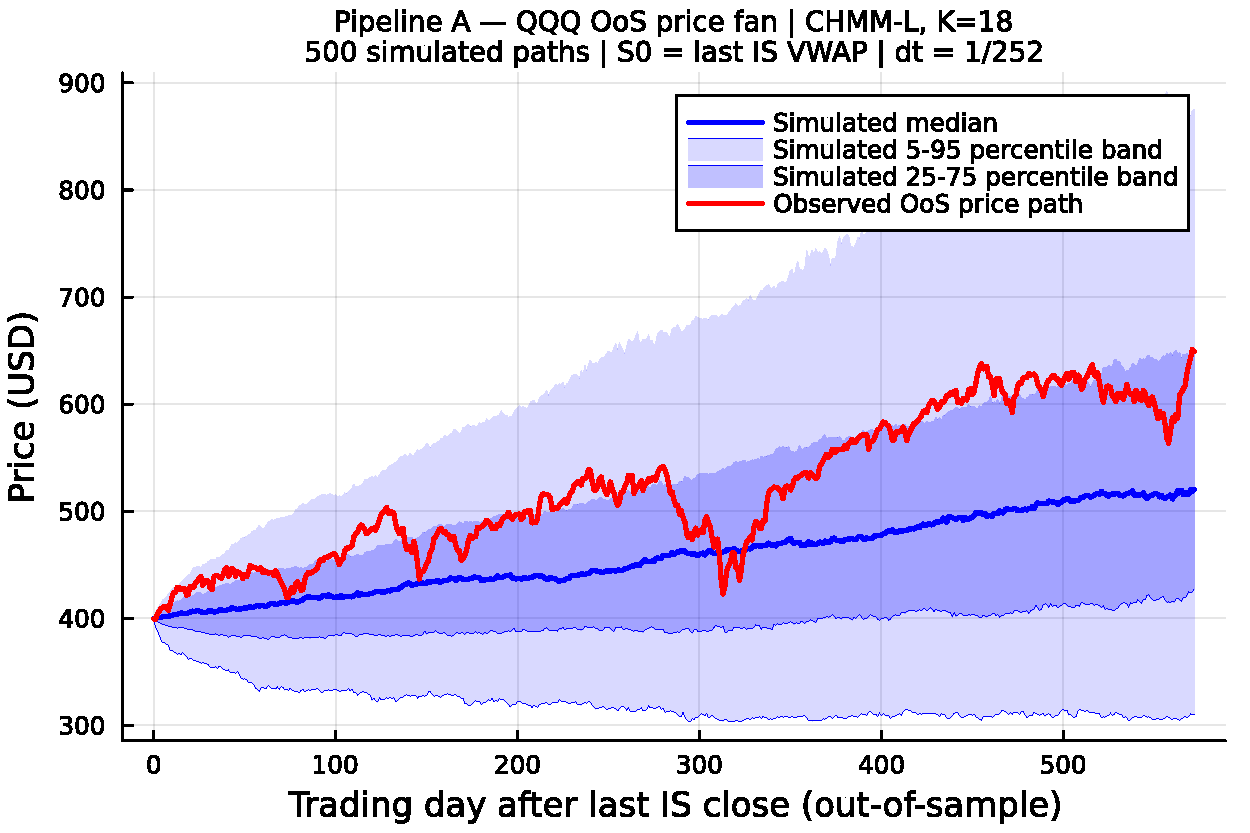
\includegraphics[width=\textwidth]{figs/Fig-QQQ-PriceFan-L.pdf}
    \caption{CHMM-L.}
\end{subfigure}
\caption{QQQ out-of-sample price fan, unconditional CHMM sampler.}
\label{fig:price_fan_qqq_appendix}
\end{figure}

\begin{figure}[h]
\centering
\begin{subfigure}[t]{0.32\textwidth}
    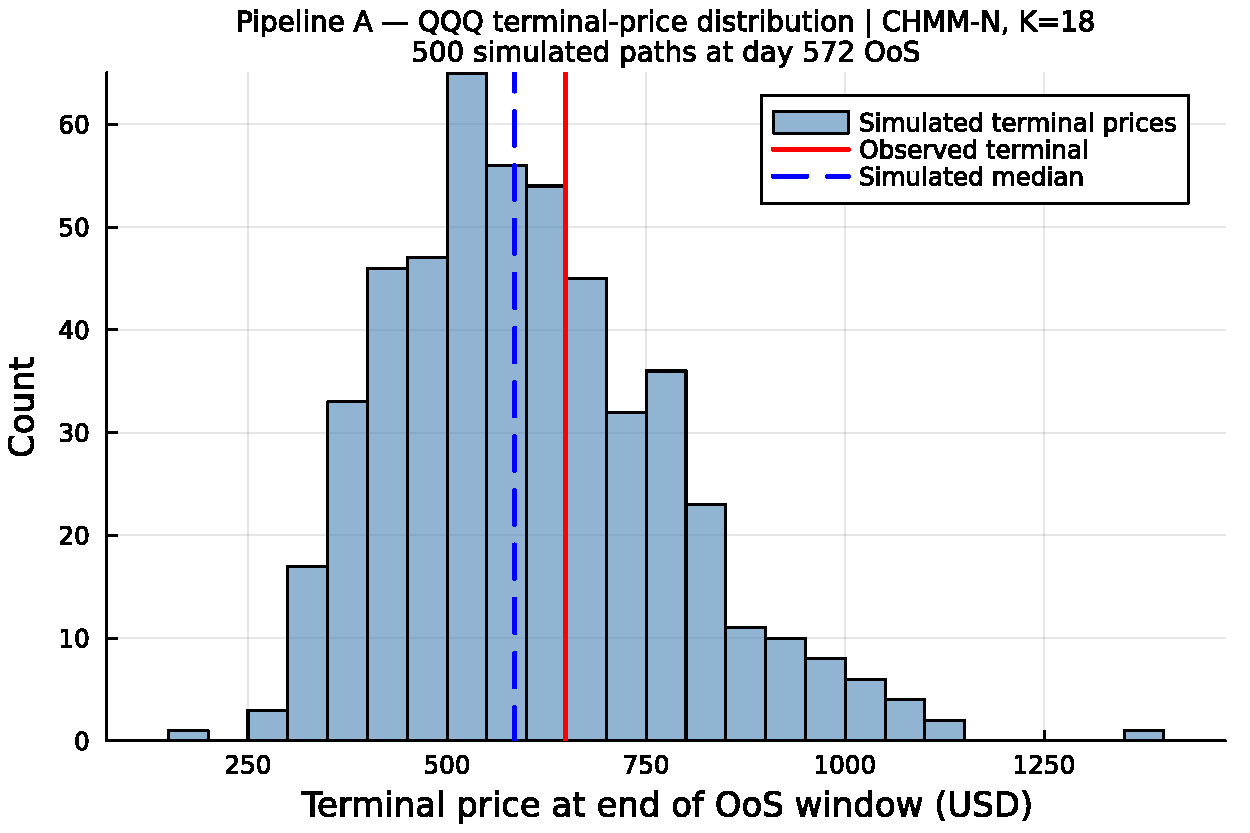
\includegraphics[width=\textwidth]{figs/Fig-QQQ-TerminalDist-N.pdf}
    \caption{CHMM-N.}
\end{subfigure}
\begin{subfigure}[t]{0.32\textwidth}
    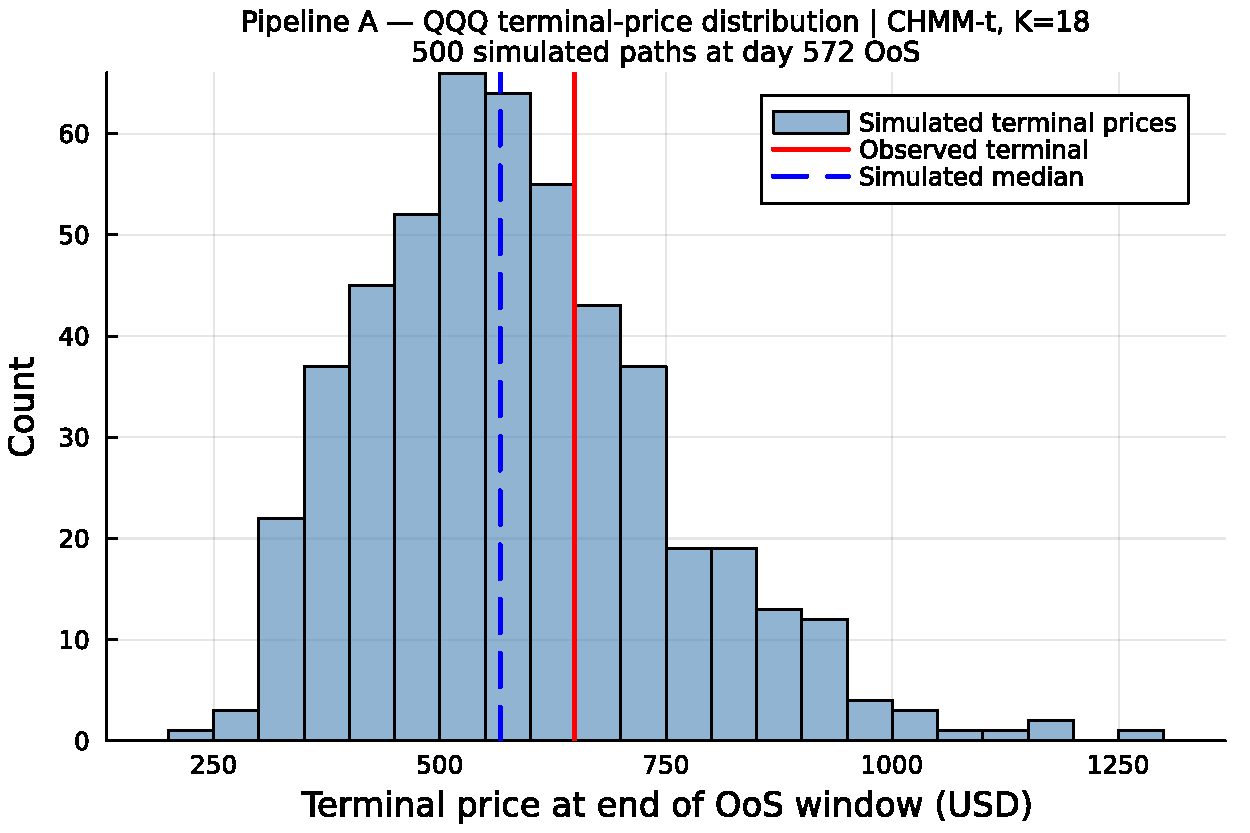
\includegraphics[width=\textwidth]{figs/Fig-QQQ-TerminalDist-t.pdf}
    \caption{CHMM-t.}
\end{subfigure}
\begin{subfigure}[t]{0.32\textwidth}
    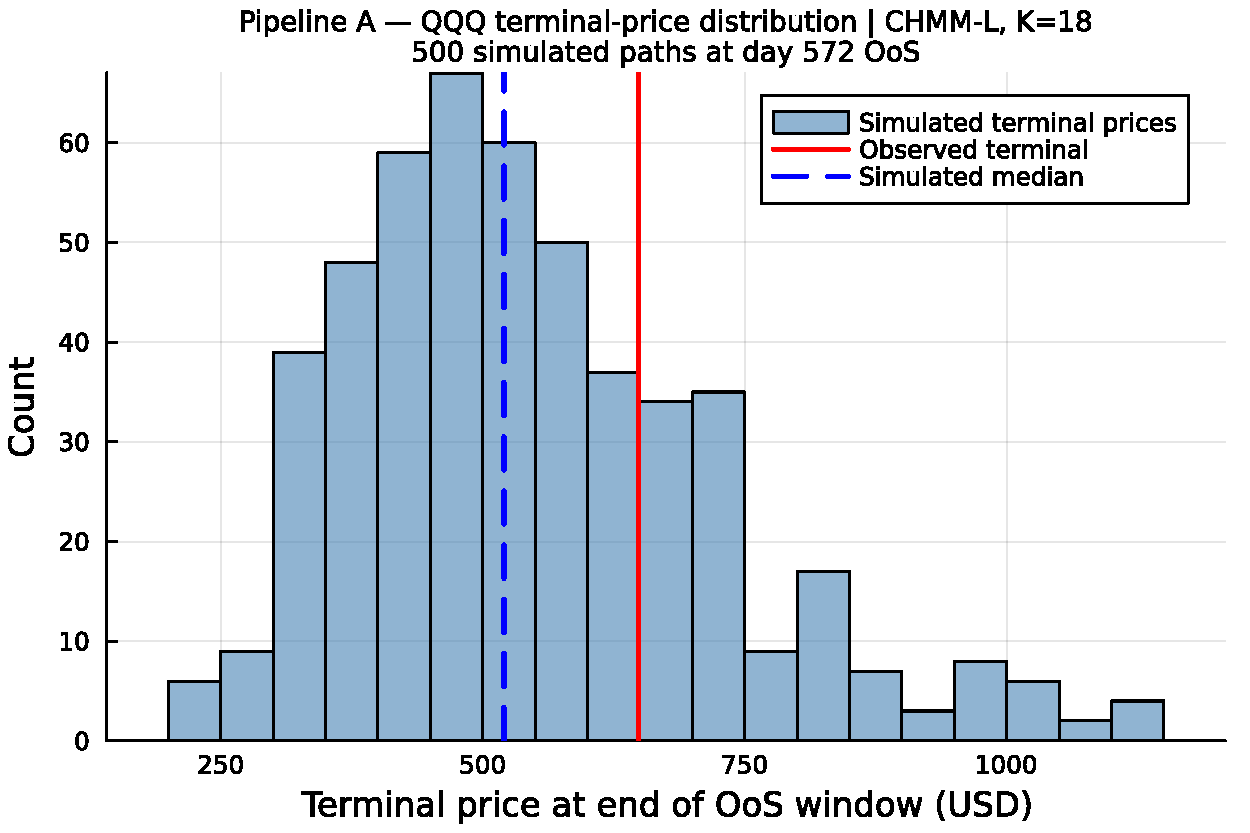
\includegraphics[width=\textwidth]{figs/Fig-QQQ-TerminalDist-L.pdf}
    \caption{CHMM-L.}
\end{subfigure}
\caption{QQQ terminal-price distribution, unconditional CHMM sampler.}
\label{fig:terminal_qqq_appendix}
\end{figure}




\subsection{Cross-Asset Dependence: Full Pipeline~B Panel}
\label{sec:supp_cross_asset}
\subsubsection{Cross-Asset Dependence Models: Derivations and Diagnostics (Pipeline~B)}
\label{sec:cross_asset_supp}

This appendix provides the technical background for the SIM and copula constructions used in Section~\ref{sec:cross_asset} of the main text. These constructions constitute \emph{Pipeline~B}: per-asset marginals come from the independent CHMMs of Pipeline~A (Section~\ref{sec:cross_asset_univariate}) and joint dependence is overlaid on top. Pipeline~A stays purely univariate; Pipeline~B is the sole multi-asset pipeline in the paper.

\paragraph{Sklar's theorem and the rank-reordering simulator.}
Sklar's theorem \cite{sklar1959fonctions, nelsen2006introduction} states that any $d$-dimensional joint CDF $H(g_1, \dots, g_d)$ with continuous marginals $F_1, \dots, F_d$ can be written as $H = C(F_1, \dots, F_d)$ for a unique copula $C$.
The rank-reordering simulator exploits this uniqueness.
If $\tilde{\mathbf{G}}$ is a matrix whose $j$-th column is an i.i.d.\ sample from $F_j$, and $\mathbf{U}$ is an independent sample from $C$, then reordering each column of $\tilde{\mathbf{G}}$ so that its ranks match $\mathbf{U}$'s produces a sample from $H$, up to discrete approximation error in the empirical ranks.
Crucially, reordering never creates new values: each column of the output is a permutation of the corresponding column of $\tilde{\mathbf{G}}$, so marginal distributions are preserved exactly \cite{iman1982distribution}.

\paragraph{Kendall's $\tau$ inversion.}
Given IS returns $\mathbf{R} \in \mathbb{R}^{T \times d}$, we estimate the pairwise Kendall's $\tau_{ij}$ from concordant/discordant pair counts and invert to the correlation scale via the analytic relationship $\rho_{ij} = \sin(\pi \tau_{ij} / 2)$, which holds exactly for the Gaussian copula family and is commonly used as a robust correlation estimator for the Student-t copula \cite{embrechts2002correlation, mcneil2015quantitative}.
The resulting matrix $\hat{\Sigma}$ is symmetric but not guaranteed positive semi-definite; we project to the nearest PSD matrix by clipping negative eigenvalues to $10^{-8}$ and rescaling the diagonal to unity.

\paragraph{Profile MLE for $\nu$.}
The Student-t copula log-density at a single pseudo-uniform observation $\mathbf{u} \in [0,1]^d$, with $x_j = t_\nu^{-1}(u_j)$ and $\mathbf{x} = (x_1, \dots, x_d)^\top$, is
\begin{align}
    \log c_t(\mathbf{u}; \Sigma, \nu)
    \;=\;&
    \log \Gamma\!\left(\tfrac{\nu+d}{2}\right)
    + (d-1)\,\log \Gamma\!\left(\tfrac{\nu}{2}\right)
    - d\,\log \Gamma\!\left(\tfrac{\nu+1}{2}\right)
    - \tfrac{1}{2} \log |\Sigma|
    \notag \\
    &\;
    - \tfrac{\nu+d}{2}\,\log\!\left(1 + \tfrac{\mathbf{x}^{\!\top} \Sigma^{-1} \mathbf{x}}{\nu}\right)
    + \sum_{j=1}^{d} \tfrac{\nu+1}{2}\,\log\!\left(1 + \tfrac{x_j^2}{\nu}\right).
    \label{eq:tcop_ll}
\end{align}
Summing over $t = 1, \dots, T$ pseudo-observations yields the profile log-likelihood as a function of $\nu$ with $\Sigma$ held fixed at the Kendall's-$\tau$ estimate.
We evaluate equation~\eqref{eq:tcop_ll} on the discrete grid $\nu \in \{2, 3, 4, 5, 6, 8, 10, 15, 20, 30\}$ and select $\hat{\nu}$ as the grid point with the largest total log-likelihood.
In Section~\ref{sec:cross_asset} the selected value was $\hat{\nu} = 6$ on the six-asset universe.

\paragraph{Sampling the copula.}
To sample $T$ rows from the $d$-dimensional Gaussian copula with correlation $\Sigma$, we (i) compute the Cholesky factor $\Sigma = L L^\top$, (ii) draw $Z \sim \mathcal{N}(0, I_d)$ i.i.d.\ and form $Y = L Z$, and (iii) return $U = \Phi(Y)$ componentwise.
For the Student-t copula with degrees of freedom $\nu$, we draw $W \sim \chi^2_\nu / \nu$ independent of $Y$ and form the multivariate-$t$ variate $X = Y / \sqrt{W}$, then return $U = t_\nu(X)$ componentwise.

\paragraph{SIM regression summary.}
Table~\ref{tab:sim_regression} reports the fitted SIM regression coefficients and goodness-of-fit statistics for the non-market assets in Section~\ref{sec:cross_asset}.
QQQ's high $R^2 = 0.840$ reflects that the Nasdaq-100 ETF is essentially a linear combination of large-cap technology names that also drive the S\&P~500 index, while JNJ's lower $R^2 = 0.260$ reflects the limited systematic exposure of low-beta healthcare stocks.
These factor loadings and residual magnitudes are what the SIM simulation re-injects at simulation time, and they explain the uneven per-asset KS pass rates reported in Table~\ref{tab:cross_asset_supp_summary}.

\begin{table}[H]
\centering
\caption{SIM regression $\hat{G}_{j,t} = \hat{\alpha}_j + \hat{\beta}_j G_{\text{SPY},t} + \hat{\eta}_{j,t}$ for the five non-market assets, fitted on the $2014$-$01$-$03$ through $2024$-$01$-$03$ IS window ($T = 2{,}516$).}
\label{tab:sim_regression}
\small
\begin{tabular}{l ccc}
\toprule
Ticker & $\hat{\alpha}$ & $\hat{\beta}$ & $R^2$ \\
\midrule
NVDA & $0.321$   & $1.694$ & $0.371$ \\
JNJ  & $0.002$   & $0.576$ & $0.260$ \\
JPM  & $-0.008$  & $1.223$ & $0.507$ \\
AAPL & $0.111$   & $1.205$ & $0.492$ \\
QQQ  & $0.047$   & $1.122$ & $0.840$ \\
\bottomrule
\end{tabular}
\end{table}

\subsubsection{Student-t Copula Profile Log-Likelihood (Pipeline~B)}
\label{sec:copula_profile_supp}

Figure~\ref{fig:copula_profile} plots the profile log-likelihood of the Student-t copula used inside Pipeline~B, computed on the six-asset SPY cross-section over the grid $\nu \in \{2, 3, 4, 5, 6, 8, 10, 15, 20, 30\}$ used in Section~\ref{sec:cross_asset}.
The curve is smooth and single-peaked, with $\nu^{*} = 6$ attaining the maximum profile log-likelihood ($6157.47$), and the neighbouring grid points $\nu = 5$ ($6143.37$) and $\nu = 8$ ($6148.37$) each within $15$ profile-log-likelihood units of the peak, indicating a shallow-but-clean optimum that agrees with the $4$--$10$ range typically reported for equity-portfolio Student-t copulas in the risk-management literature.

\begin{figure}[h]
\centering
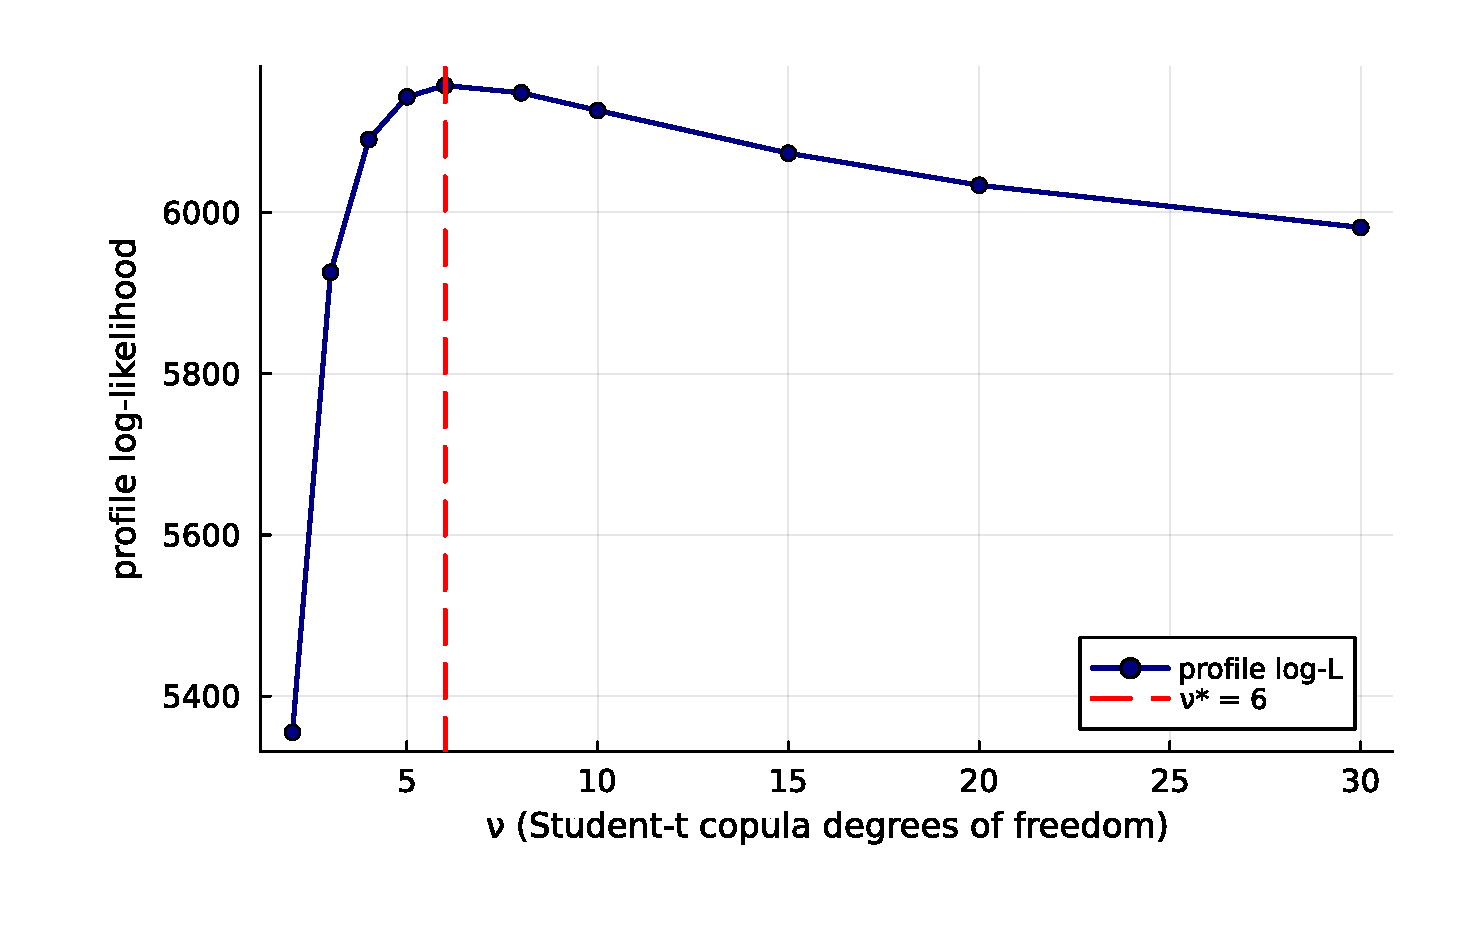
\includegraphics[width=0.70\textwidth]{figs/Fig-Copula-Profile.pdf}
\caption{\textbf{Profile log-likelihood of the Student-t copula} used inside Pipeline~B on the six-asset SPY cross-section (SPY, NVDA, JNJ, JPM, AAPL, QQQ; IS window 2014-01-03 through 2024-01-03). The vertical axis is the profile log-likelihood evaluated at each degrees-of-freedom value $\nu$ on the grid $\{2, 3, 4, 5, 6, 8, 10, 15, 20, 30\}$; the dashed red line marks the profile MLE $\nu^{*} = 6$ (peak value 6157.47). The CHMM-N marginals are held fixed at the Pipeline~A per-asset fits while $\nu$ is varied.}
\label{fig:copula_profile}
\end{figure}

\subsubsection{Cross-Asset Correlation Heat Maps (Pipeline~B, Companion to Table~\ref{tab:cross_asset_supp_summary})}
\label{sec:cross_asset_corr_supp}

Figure~\ref{fig:cross_asset_corr} visualises the observed and path-averaged simulated correlation matrices for the dependence models of Section~\ref{sec:cross_asset}.
The panel ordering is SIM, Gaussian copula, Student-t copula (each reported quantitatively in Table~\ref{tab:cross_asset_supp_summary}), plus a truncated C-vine variant with SPY as root for visual comparison.
All five panels share the six-asset SPY cross-section and the same CHMM-N marginals at $K = 18$, so any visible differences between the simulated panels reflect only the dependence construction.

\begin{figure}[H]
\centering
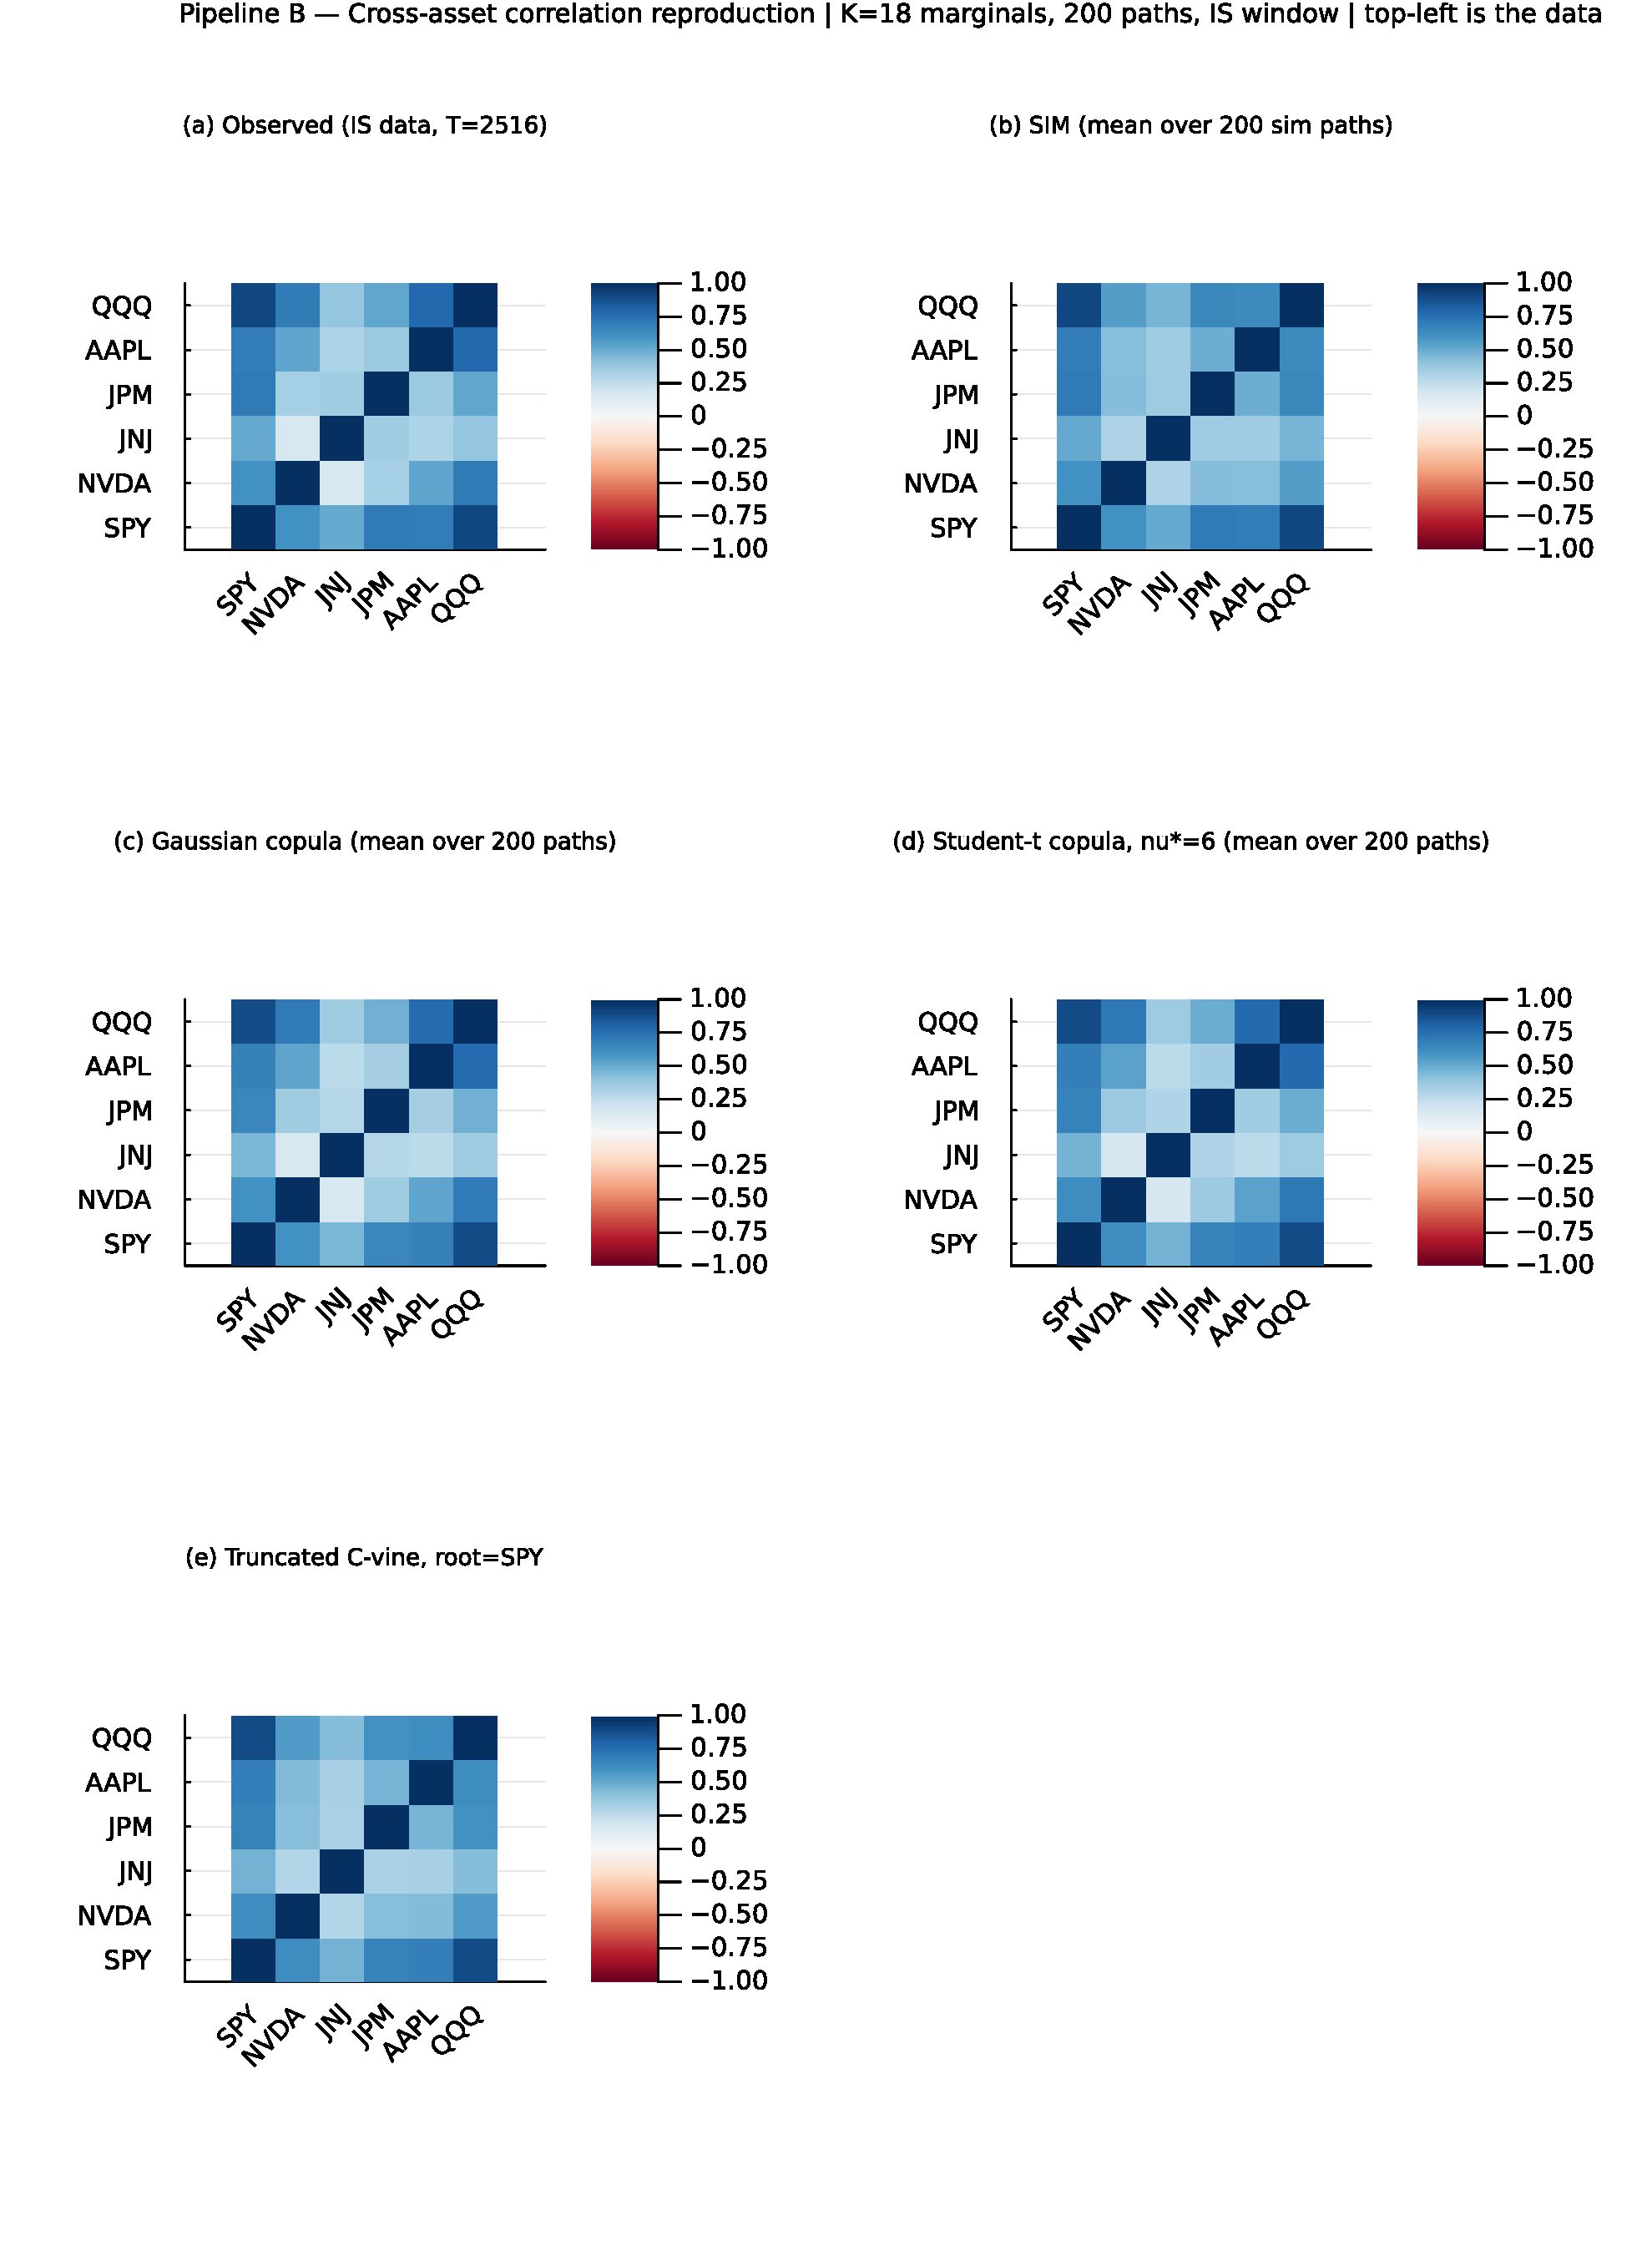
\includegraphics[width=0.75\textwidth]{figs/Fig-Cross-Asset-Correlation.pdf}
\caption{\textbf{Cross-asset IS correlation reproduction across dependence models} (Pipeline~B, companion to Table~\ref{tab:cross_asset_supp_summary}). Panel~(a), top-left: \emph{observed} correlation matrix on 2014-01-03 through 2024-01-03 daily excess log returns for SPY, NVDA, JNJ, JPM, AAPL, QQQ (IS window, $T_{\text{IS}} = 2{,}516$). Panel~(b), top-right: path-averaged correlation under the Single Index Model with SPY as market factor. Panel~(c), middle-left: path-averaged correlation under the Gaussian copula on CHMM marginals. Panel~(d), middle-right: path-averaged correlation under the Student-t copula on CHMM marginals, $\nu^* = 6$. Panel~(e), bottom-left: path-averaged correlation under a truncated C-vine copula with SPY as root. Each simulated panel averages over 200 paths of length $T_{\text{IS}}$. All marginals are the per-asset CHMM-N fits at $K = 18$ from Table~\ref{tab:cross_asset}; color scale in $[-1, 1]$, red-white-blue (RdBu) diverging. Closer visual match to panel~(a) is better.}
\label{fig:cross_asset_corr}
\end{figure}

\subsubsection{Non-US Asset Class Extension and Per-Pair OoS Off-Diagonal Breakdown}
\label{sec:non_us_asset_supp}

The body universe (SPY, NVDA, JNJ, JPM, AAPL, QQQ) is six US-listed equity tickers from one country-index family. To probe whether the cross-asset construction generalises off the equity cluster we extend the universe with GLD (SPDR Gold Trust), a US-listed ETF whose underlying is physically-backed gold, i.e.\ a non-equity commodity asset class.

\paragraph{GLD Pipeline-A univariate fidelity.}
Fitting CHMM-N, CHMM-t, and CHMM-L on the GLD return series at $K = 18$ produces $100\%$ IS KS pass rate for all three families and observed IS excess kurtosis $3.6$ matched closely by CHMM-L ($2.2$); on OoS, however, the KS pass rate collapses to $0\%$ for all three families against an observed OoS excess kurtosis of $6.5$. Inspection of the GLD price path on the $2024$--$2026$ OoS window shows the asset re-priced from $\sim 200$ to $\sim 300$ on a persistent demand shock not represented in the $2014$--$2024$ IS regime library. This is the same stationarity-scope artefact as the NVDA / JPM single-name OoS cliffs reported in Section~\ref{sec:cross_asset_univariate}, on a non-equity asset; the limitation is not equity-specific.

\paragraph{Pipeline-B: 7-ticker Student-t copula off-diagonal MAE.}
Refitting the Student-t copula on the augmented seven-ticker universe at $\nu^\star = 6$ gives IS off-diagonal MAE of $0.029$ (six-ticker baseline: $0.027$) and OoS off-diagonal MAE of $0.179$ (six-ticker baseline: $0.211$). Adding the low-equity-correlation gold ETF \emph{reduces} the OoS off-diagonal MAE, because the equity-cluster correlation degradation is the dominant component; pairs involving GLD have moderate IS-to-OoS shifts ($|\Delta| \in [0.04, 0.19]$) while the largest equity-cluster pairs (JNJ-QQQ, SPY-JNJ, NVDA-JNJ) have $|\Delta| > 0.48$ on OoS.

\paragraph{Per-pair OoS gap localisation.}
Table~\ref{tab:per_pair_offdiag_mae} reports the per-pair off-diagonal absolute deviation between observed and path-averaged simulated correlation matrices on IS and OoS, sorted by OoS $|\Delta|$. The OoS gap concentrates in pairs involving JNJ (the defensive single-name proxy): JNJ's IS correlation with the broad equity factor (QQQ, SPY) collapses on OoS, in some pairs flipping sign, and the IS-fixed copula has no mechanism for tracking that shift. The gold-ETF pairs (SPY-GLD, JPM-GLD, JNJ-GLD, QQQ-GLD) sit in the middle of the ranking with $|\Delta|$ between $0.10$ and $0.19$ on OoS. The dominant cause of the OoS off-diagonal gap is therefore neither equity-cluster size nor copula-degree mis-specification but a single-name regime shift in the JNJ-equity-factor relationship that the IS-fitted dependence layer cannot anticipate.

\begin{table}[t]
\centering
\small
\caption{\textbf{Per-pair off-diagonal correlation MAE on the seven-ticker universe} (Pipeline B, Student-t copula on CHMM-N marginals at $K = 18$, $200$ paths, $\nu^\star = 6$). For each ticker pair $(i, j)$ the table reports $|\Sigma_{\text{sim,avg}}[i,j] - \Sigma_{\text{obs}}[i,j]|$ on IS and OoS, ranked by OoS $|\Delta|$. Only the ten largest-OoS-gap pairs are shown for compactness.}
\label{tab:per_pair_offdiag_mae}
\begin{tabular}{l c c c}
\toprule
Pair & IS $|\Delta|$ & OoS $|\Delta|$ & OoS $-$ IS \\
\midrule
JNJ-QQQ   & $0.027$ & $0.544$ & $0.517$ \\
SPY-JNJ   & $0.037$ & $0.509$ & $0.473$ \\
NVDA-JNJ  & $0.017$ & $0.489$ & $0.473$ \\
NVDA-AAPL & $0.011$ & $0.278$ & $0.268$ \\
JNJ-JPM   & $0.046$ & $0.261$ & $0.216$ \\
JNJ-AAPL  & $0.042$ & $0.244$ & $0.202$ \\
AAPL-QQQ  & $0.003$ & $0.227$ & $0.224$ \\
JPM-GLD   & $0.027$ & $0.187$ & $0.160$ \\
SPY-GLD   & $0.038$ & $0.127$ & $0.089$ \\
JNJ-GLD   & $0.015$ & $0.117$ & $0.101$ \\
\bottomrule
\end{tabular}
\end{table}




\subsection{\texorpdfstring{Pre-OoS Validation $K$-Selection, Walk-Forward Summary, and $\nu_k$ Diagnostics}{Pre-OoS Validation K-Selection, Walk-Forward Summary, and nu\_k Diagnostics}}
\label{sec:supp_misc}

\paragraph{Pre-OoS validation $K$-selection.}
The $K = 18$ operating point in the main panel was chosen via a multi-objective criterion combining information-criterion (IC) rank with IS and OoS distributional pass rates, which uses the same $2024$--$2026$ window later used for VaR. As a clean re-selection that decouples the two, we fit CHMM-N on $2014$-$01$-$03$ through $2021$-$12$-$31$ ($n = 2{,}013$) and score every $K$ in the sweep by the forward-algorithm held-out log-likelihood on $2022$-$01$-$03$ through $2024$-$01$-$03$ ($n = 502$); the $2024$--$2026$ window is not touched. Held-out log-lik, BIC, HQC, and CAIC all select $K^\star = 3$ (per-observation log-lik $-2.5345$ at $K = 3$ vs.\ $-2.5694$ at $K = 18$); AIC selects $K^\star = 6$; held-out two-sample KS selects $K^\star = 9$. None of the six criteria that avoid the OoS window select $K = 18$. The $K = 18$ choice is best read as a multi-metric one that weights tail fidelity (kurtosis, AD) and downstream VaR behaviour alongside likelihood; a parallel main panel at $K = 3$ would re-rank some rows in CHMM's favour on ACF-MAE and against it on tail fidelity. The $2022$--$2023$ validation slice is itself partly a structural-break period (the rate-hike cycle), so any model with substantial IS-specific structure generalises worse on it.

\paragraph{$\nu_k$ bracket and penalised-ECM rate sweep.}
A bracket sweep $\nu_{\min} \in \{2.1, 2.5, 3.0, 4.0\}$ shows the CHMM-t fit does not pile against the lower bracket: median $\nu_k = 50$, only $2/18$ states near the lower edge. Lifting $\nu_{\min}$ does not reduce the $14.30 \to 7.69$ overshoot because the fit shifts posterior mass into the newly-recentred tail states. An exponential $1/\nu_k$ shrinkage prior at rate $\lambda \in \{0, 5, 20, 50, 100, 200\}$ reduces simulated excess kurtosis monotonically: $14.30, 11.19, 8.43, 5.41, 3.96, 3.67$. The recommended rate $\lambda = 20$ brings simulated kurtosis to $\approx 8$ (close to the observed $7.69$) at a $1$pp IS KS cost. Only the $\nu_{\min}$ state parameter actually moves ($2.1 \to 4.89$); upper bracket and median remain at $50$. The overshoot is therefore a single-state artefact of the two tail regimes hitting the lower bracket under unpenalised ECM.

\paragraph{Cross-asset summary.}
The full per-construction Pipeline~B panel is in Section~\ref{sec:supp_cross_asset}; for reference, the headline ordering is summarised in Table~\ref{tab:cross_asset_supp_summary}.

\begin{table}[h]
\centering
\small
\caption{\textbf{Cross-asset dependence summary} (Pipeline~B; CHMM-N marginals at $K = 18$; $200$ paths). Median per-asset KS pass rate (\%) and off-diagonal MAE of the simulated correlation matrix vs.\ observed. The Student-t copula at $\nu^\star = 6$ is the strongest dependence layer on every IS metric; full per-asset detail is in Section~\ref{sec:supp_cross_asset}.}
\label{tab:cross_asset_supp_summary}
\begin{tabular}{l c c c c}
\toprule
& Median IS KS & Median OoS KS & Off-diag MAE IS & Off-diag MAE OoS \\
\midrule
Single Index Model       & $78.5$  & $85.0$  & $0.076$ & $0.261$ \\
Gaussian copula          & $97.8$  & $87.2$  & $0.031$ & $0.202$ \\
Student-t copula ($\nu^\star = 6$) & $\mathbf{96.0}$  & $\mathbf{89.8}$  & $\mathbf{0.027}$ & $\mathbf{0.208}$ \\
\bottomrule
\end{tabular}
\end{table}


\end{document}
